% ============================================================
%  JMP_V11.tex  — "Revisiting the global distribution of climate damages"
%  Romain Fillon  |  AER working-paper format
%  Compiled by tools/compiler.py from the package root (see README, Check)
% ============================================================

\documentclass[12pt]{article}

%% --- Layout ---
\usepackage[letterpaper, top=1in, bottom=1in, left=1in, right=1in]{geometry}
\usepackage{setspace}

%% --- Fonts ---
\usepackage[T1]{fontenc}
\usepackage[utf8]{inputenc}
\usepackage{times}
\usepackage{setspace}
%% --- Math ---
\usepackage{amsmath}
\usepackage{amssymb}

%% --- Tables & Figures ---
\usepackage{booktabs}
\usepackage{tabularx}
\usepackage{array}
\usepackage{graphicx}
\graphicspath{{output/}}
\usepackage{float}
\usepackage{subfigure}

%% --- References ---
\usepackage{natbib}
\usepackage[english]{babel}

%% --- Hyperlinks (load after natbib) ---
\usepackage[colorlinks=true, urlcolor=purple, linkcolor=blue,
            citecolor=violet]{hyperref}

%% --- Theorems ---
\usepackage{amsthm}
\newtheorem{proposition}{Proposition}
\newtheorem{corollary}{Corollary}[proposition]

%% --- Misc ---
\usepackage{lscape}
\usepackage{indentfirst}
\usepackage{authblk}
\usepackage{comment}
\usepackage{xcolor}
\usepackage{lineno}
\renewcommand\Affilfont{\fontsize{8}{10.8}\itshape}

%% ----------------------------------------------------------------
%%  Title block
%% ----------------------------------------------------------------
\title{Revisiting the Global Distribution of Climate Damages}

\author[1,2]{Romain Fillon}
\affil[1]{ Paris-Saclay Applied Economics, Graduate School of Economics
  and Management, 
   Universit\'e Paris-Saclay, France}
\affil[2]{ Centre International de Recherche sur l'Environnement et le D\'eveloppement, CIRED,  Universit\'e Paris-Saclay, France}
\date{ October 2026}

%% ----------------------------------------------------------------
%% All computed magnitudes of the paper. GENERATED, do not edit:
%%   02_GE/emit_values.py
%% A macro that is not emitted shows as \PROVISOIRE (??) plus a LaTeX warning.
% ====================================================================
% GENERATED by 02_GE/emit_values.py
% DO NOT EDIT BY HAND. Every GE value in the paper comes from here.
% terminal horizon = the last transition (2095-2099), labelled 2100.
% --------------------------------------------------------------------
%% PROVENANCE BY MACRO FAMILY
%   CAP_TAG (filename suffix) : ''
%   ARM AS RECORDED IN output/ge_runs_manifest.csv : SANS cap de column-mass (cap_colmass=none)
%%   (the suffix names a file; only the manifest says what the solver did)
%
% (!) HOMOGENEOUS OVERRIDE ARM: everything is read from output.
%   The vintages below describe the headline arm, not this one.
%
% headline         GEnorth* GEagg* GEcty* GEtier* GEpopLoss* GEpopGain* GEnorthLat*
%   runs_dir : output
%   vintage  : 1 run_id for the 3 file(s) read (named in ge_runs_manifest.csv)
%
% endogenous channel GEchanIncomeTrop GEchanIncomeMid GEchanIncomeSub GEchanIncomeArc
%   runs_dir : output
%   vintage  : no file in the manifest (+2 outside the manifest: amenity_hat_path_sc2_q50.csv, amenity_hat_path_sc3_q50.csv)
%
% null arm g=0     GEsensNorthLo GEsensPreserved* + columns g^LB=0 of tab_ge_north_sens and row " Lower bound " of tab_ge_sensitivity
%   runs_dir : output
%   vintage  : 1 run_id for the 3 file(s) read (named in ge_runs_manifest.csv)
%
% mask decomposition GEmask*
%   runs_dir : via decompose_metric_channels.py (md5 pinned)
%   vintage  : via decompose_metric_channels.py (md5 pinned)
%
% sc4 channels     GEnorthChanEval GEnorthChanShape
%   runs_dir : via decompose_metric_channels.py (md5 pinned)
%   vintage  : via decompose_metric_channels.py (md5 pinned)
%
% --------------------------------------------------------------------
% RUN GRID : 78 file(s) in the manifest, 1 run_id (named in ge_runs_manifest.csv)
%   cap_colmass : none
%   amenity_spec: (empty = null), baseline
% ====================================================================

% ---- guardrail: any macro not emitted shouts ----
\providecommand{\PROVISOIRE}{\textbf{??}\PackageWarning{values}{PROVISOIRE: value not emitted}}

% ---- grid and run constants (derived, never typed) ----
\newcommand{\GEncells}{13{,}986}
\newcommand{\GEncellsPotential}{17{,}048}
\newcommand{\GEnperiods}{17}
\newcommand{\GEntransitions}{16}
\newcommand{\GEnsspOneModel}{11}
\newcommand{\GEnsspTwoModels}{164}
\newcommand{\GEnsspThreeModels}{1}
% GEhorizonLabel is an ETIQUETTE, not a year the model indexes on:
% the terminal row is the transition 2095-2099.
\newcommand{\GEhorizonLabel}{2100}
\newcommand{\GEhorizonSpan}{2015--2100}
\newcommand{\GEcmipModels}{GFDL-ESM4, IPSL-CM6A-LR, MPI-ESM1-2-HR and MRI-ESM2-0}
% GEdensityCut is the cut the CODE applies: population > 1 inhabitant
% per CELL (02a_calibration_at_1deg.r l.302-305), intersected with
% wage > 0 and productivity > 0. It is NOT the 0.1/km2 of the prose,
% which governs lambda and not the cell mask, and it is NOT binding:
% the population test alone would keep GEncellsPopOnly cells.
\newcommand{\GEdensityCut}{1}
\newcommand{\GEdensityCutUnit}{inhabitant per cell}
\newcommand{\GEncellsPopOnly}{14{,}055}
% GEtheta: param_theta of 02c_model/specification_study.csv, the
% ONLY source of the constant. The solver applies it in
% trade_weights = (Z/x)^theta; the estimation divides by it
% (SCALE_PROD = 1/THETA_GE). The .tex must never copy it.
\newcommand{\GEtheta}{6.5}
\newcommand{\GEnruns}{78}
\newcommand{\GEarmLabel}{SANS cap de column-mass (cap_colmass=none)}
\newcommand{\GEamenitySpec}{interior amenity estimate $\hat f_a^{\,q50}$}
\newcommand{\GEamenitySpecBody}{amenity lower bound $f_a = 0$}

% ---- initial calibrated state (lambda_0, mu_0) ----
% Source: output/ge_calib_diagnostic.csv, written once by
% 02_GE/ge_calibration_diagnostic.py, which IMPORTS the solver's own
% loaders (load_h5, load_migration). The emitter never reads lambda.h5:
% 867 MB and 37 s measured, for statistics that describe the INPUT
% matrices and do not depend on the run.
\newcommand{\GElamDiagMedian}{1.00}
\newcommand{\GElamDiagMean}{1.00}
\newcommand{\GElamDiagShareHigh}{97.1}
\newcommand{\GEimportShareMean}{0.4}
\newcommand{\GEclearMedian}{1.00}
\newcommand{\GEclearGap}{0}
\newcommand{\GEclearLo}{\PROVISOIRE}
\newcommand{\GEclearHi}{\PROVISOIRE}
\newcommand{\GEmigSenders}{PAK, BGD, SYR, IND, CHN}
\newcommand{\GEmigReceivers}{USA, SAU, DEU, TUR, ARE}
\newcommand{\GEdomCellsOut}{916}
\newcommand{\GEdomPopOutM}{142.5}
\newcommand{\GEdomPopOutShare}{1.9}
\newcommand{\GEdomCtyOutN}{39}
\newcommand{\GEdomCtyOutPopM}{18.2}
\newcommand{\GEdomCtyPartialN}{100}
\newcommand{\GEdomMigLostM}{7.6}
% 2 macro(s) NOT EMITTED for lack of a producer: GEclearLo, GEclearHi
\newcommand{\GEmigInternalCrossM}{5.73}
\newcommand{\GEmigInternalCrossShare}{6.4}
\newcommand{\GEcapColmass}{none}
% GEborderShare: NOT EMITTED -- no archived artefact carries the
% border-cell classification, and inventing a definition here would
% be a new result, not an emission.
\newcommand{\GEborderShare}{\PROVISOIRE}

% ---- North aggregate >= 45N (headline) ----
\newcommand{\GEnorthAnnual}{+0.0115}
\newcommand{\GEnorthDailyExtra}{-0.0178}
\newcommand{\GEnorthNet}{-0.0063}
\newcommand{\GEnorthPopLoss}{99.5}
\newcommand{\GEnorthPopM}{662}
\newcommand{\GEnorthAnnualQfifty}{-0.048}
\newcommand{\GEnorthNetQfifty}{-0.107}
\newcommand{\GEnorthLatLastNeg}{66.5}
\newcommand{\GEnorthLatAllNeg}{true}
\newcommand{\GEnorthLatLastNegPopM}{2.1}
\newcommand{\GEnorthLatLastNegDaily}{-0.0001}
% GEnorthLatAllNeg=true : the daily total is negative at EVERY threshold of the latitude grid.
\newcommand{\GEnorthArcticPopM}{2.1}
\newcommand{\GEnorthNcty}{7}
\newcommand{\GEnorthNGain}{6}
\newcommand{\GEnorthNExtraNeg}{7}
\newcommand{\GEnorthExceptions}{France}

% ---- aggregation gap decomposition (sc4) ----
\newcommand{\GEnorthChanEvalQfifty}{-0.013}
\newcommand{\GEnorthChanShapeQfifty}{-0.046}
\newcommand{\GEnorthChanEval}{+0.0034}
\newcommand{\GEnorthChanShape}{-0.0211}
\newcommand{\GEnorthChanRatio}{6.3}
\newcommand{\GEnorthChanSameSign}{of opposite sign to}
\newcommand{\GEworldChanEval}{+0.001}
\newcommand{\GEworldChanShape}{-0.011}

% ---- world aggregate, three horizons ----
% Thirty=2030, Fifty=2050, Hundred=2100 (digits are
% barred from a macro name). 'Hundred' is a NAME, kept stable across
% every relabelling so no call site in the manuscript has to move.
\newcommand{\GEaggDailyThirty}{-0.003}
\newcommand{\GEaggAnnualThirty}{-0.001}
\newcommand{\GEaggExtraThirty}{-0.002}
\newcommand{\GEaggDailyFifty}{-0.010}
\newcommand{\GEaggAnnualFifty}{-0.004}
\newcommand{\GEaggExtraFifty}{-0.005}
\newcommand{\GEaggDailyHundred}{-0.017}
\newcommand{\GEaggAnnualHundred}{-0.008}
\newcommand{\GEaggExtraHundred}{-0.010}
\newcommand{\GEampRatio}{124.7}
\newcommand{\GEaggAnnualThirtyPct}{-0.1}
\newcommand{\GEpopLossDaily}{99.9}
\newcommand{\GEpopLossAnnual}{88.3}
\newcommand{\GEpopLossExtra}{72.2}
\newcommand{\GEpopGainDaily}{0.1}
\newcommand{\GEpopGainAnnual}{11.7}

% ---- countries: reversals / amplifications / France ----
\newcommand{\GEctyRusNet}{-0.003}
\newcommand{\GEctyRusAnnual}{+0.025}
\newcommand{\GEctyRusDailyExtra}{-0.028}
\newcommand{\GEctyFinNet}{-0.001}
\newcommand{\GEctyFinAnnual}{+0.027}
\newcommand{\GEctyFinDailyExtra}{-0.028}
\newcommand{\GEctyNorNet}{-0.005}
\newcommand{\GEctyNorAnnual}{+0.013}
\newcommand{\GEctyNorDailyExtra}{-0.018}
\newcommand{\GEctySweNet}{-0.004}
\newcommand{\GEctySweAnnual}{+0.012}
\newcommand{\GEctySweDailyExtra}{-0.017}
\newcommand{\GEctyCanNet}{-0.010}
\newcommand{\GEctyCanAnnual}{+0.011}
\newcommand{\GEctyCanDailyExtra}{-0.021}
\newcommand{\GEctyDeuNet}{-0.007}
\newcommand{\GEctyDeuAnnual}{+0.004}
\newcommand{\GEctyDeuDailyExtra}{-0.011}
\newcommand{\GEctyFraNet}{-0.012}
\newcommand{\GEctyFraAnnual}{-0.008}
\newcommand{\GEctyFraDailyExtra}{-0.004}

% ---- 1990 GDP per capita quartiles ----
\newcommand{\GEtierQoneDaily}{-0.024}
\newcommand{\GEtierQoneAnnual}{-0.008}
\newcommand{\GEtierQoneExtra}{-0.016}
\newcommand{\GEtierQtwoDaily}{-0.014}
\newcommand{\GEtierQtwoAnnual}{-0.012}
\newcommand{\GEtierQtwoExtra}{-0.002}
\newcommand{\GEtierQthreeDaily}{-0.019}
\newcommand{\GEtierQthreeAnnual}{-0.009}
\newcommand{\GEtierQthreeExtra}{-0.010}
\newcommand{\GEtierQfourDaily}{-0.011}
\newcommand{\GEtierQfourAnnual}{-0.003}
\newcommand{\GEtierQfourExtra}{-0.008}
\newcommand{\GEtierExtraRatio}{0.5}

% ---- endogenous income channel by latitude band ----
% The only publishable channel object: robust to the hat-path orientation.
% Neither the amplification ratio (not robust) nor the quartile (wrong axis).
\newcommand{\GEchanIncomeTrop}{-0.012}
\newcommand{\GEchanIncomeMid}{-0.002}
\newcommand{\GEchanIncomeSub}{-0.019}
\newcommand{\GEchanIncomeArc}{-0.037}

% ---- source decomposition by exposure masks (f_a = 0, central draw) ----
\newcommand{\GEmaskNorthWarmingExtraShare}{91.8}
\newcommand{\GEmaskNonNorthWarmingExtraShare}{8.1}
\newcommand{\GEmaskNorthWarmingIncomeSubShare}{95.8}
\newcommand{\GEmaskNorthWarmingIncomeArcShare}{98.5}
\newcommand{\GEmaskNorthWarmingAnnual}{+0.014}
\newcommand{\GEmaskNorthWarmingDaily}{-0.002}
\newcommand{\GEmaskNonNorthWarmingDailyShare}{68.9}
\newcommand{\GEmaskInteractionMaxShare}{0.07}
\newcommand{\GEmaskNorthCells}{4{,}581}
\newcommand{\GEmaskNonNorthCells}{9{,}405}

% ---- colmass lambda0 / mu0 (app:ge_robustness) ----
\newcommand{\CALIBlamMaxColmass}{7}
\newcommand{\CALIBmuMaxColmass}{8.2}

% ---- amenity range (lower bound g=0 against the interior g=q50) ----
% NET North aggregate (daily margin), bounded between the two amenity specs.
% Lo/Hi = numerical min/max (both bounds are net losses).
\newcommand{\GEsensNorthLo}{-0.107}
\newcommand{\GEsensNorthHi}{-0.006}
% Share of the AGGREGATE North magnitude preserved under g=0 (min/max over the three margins).
\newcommand{\GEsensPreservedLo}{-24\%}
\newcommand{\GEsensPreservedHi}{30\%}
% Same AT COUNTRY LEVEL (extra margin, 6 cold economies): lower than the aggregate.
\newcommand{\GEsensPreservedCtyLo}{26\%}
\newcommand{\GEsensPreservedCtyHi}{40\%}
% How much deeper the INTERIOR arm is than the lower
% bound, North >= 45N. Ratio of magnitudes of the same sign.
\newcommand{\GEsensNetRatio}{17.1}
\newcommand{\GEsensExtraRatio}{3.3}

% ---- lower bound f_a=0 vs interior f_a^q50 (S5) ----
\newcommand{\GEworldDaily}{-0.017}
\newcommand{\GEworldAnnual}{-0.008}
\newcommand{\GEworldExtra}{-0.010}
\newcommand{\GEnorthExtraLB}{-0.018}
\newcommand{\GEnorthNetLB}{-0.006}
\newcommand{\GEworldDailyQfifty}{-0.218}
\newcommand{\GEworldAnnualQfifty}{-0.153}

% ---- MC band on the dose-responses: q05 / q50 / q95 ----
% WHAT Qlo AND Qhi NAME. Qlo is the aggregate evaluated on the q05
% COLUMN of the dose-response tables, Qhi on the q95 column. They name
% the quantile of the CURVE, not a sorted bound on this aggregate: the
% columns are POINTWISE quantiles across MC draws (lib_drf.R,
% mc_summarise: quantile(y,.05) by x), so no single draw traces them and
% a functional of such an envelope is not a quantile of that
% functional's distribution. The median is NOT guaranteed to lie
% between Qlo and Qhi. Do not caption these as a confidence band.
% MARGIN: daily extra (sc2/sc3) -- the only margin whose numerator and
% denominator are evaluated at the same severity level, so the severity
% assumption differences out of the comparison between metrics.
% Same path as the median for every column: aggregates_for(), same cell
% mask, same weights, same cumulation, same terminal period; the q50
% column is checked against the module aggregates to fp identity.
% AMENITY OF THE BAND RUNS, read from the manifest: baseline.
\newcommand{\GEworldExtraQfifty}{-0.065}
\newcommand{\GEworldExtraQlo}{-0.049}
\newcommand{\GEworldExtraQhi}{-0.040}
\newcommand{\GEnorthExtraQfifty}{-0.059}
\newcommand{\GEnorthExtraQlo}{-0.103}
\newcommand{\GEnorthExtraQhi}{-0.022}
\newcommand{\GElatFFExtraQfifty}{-0.072}
\newcommand{\GElatFFExtraQlo}{-0.116}
\newcommand{\GElatFFExtraQhi}{-0.023}
\newcommand{\GElatAExtraQfifty}{-0.092}
\newcommand{\GElatAExtraQlo}{-0.150}
\newcommand{\GElatAExtraQhi}{-0.026}
\newcommand{\GEctyRusExtraQfifty}{-0.081}
\newcommand{\GEctyRusExtraQlo}{-0.133}
\newcommand{\GEctyRusExtraQhi}{-0.025}
\newcommand{\GEctyFinExtraQfifty}{-0.071}
\newcommand{\GEctyFinExtraQlo}{-0.090}
\newcommand{\GEctyFinExtraQhi}{-0.021}
\newcommand{\GEctyCanExtraQfifty}{-0.073}
\newcommand{\GEctyCanExtraQlo}{-0.117}
\newcommand{\GEctyCanExtraQhi}{-0.034}
\newcommand{\GEctyDeuExtraQfifty}{-0.041}
\newcommand{\GEctyDeuExtraQlo}{-0.092}
\newcommand{\GEctyDeuExtraQhi}{-0.014}
% Share of world population GAINING on the daily-extra margin.
\newcommand{\GEpopGainExtra}{3.6}
\newcommand{\GEpopGainExtraQlo}{24.0}
\newcommand{\GEpopGainExtraQhi}{9.8}
% RANGE of the Northern DAILY TOTAL across the three solves. Not a
% band: the extremes of three runs, reported as an extent.
\newcommand{\GEnorthDailyRunMin}{-0.157}
\newcommand{\GEnorthDailyRunMax}{-0.017}
\newcommand{\GEnorthDailyRunAllNeg}{negative in all three}
% 2 unit(s) with the median OUTSIDE [q05, q95]: world, popGain
\newcommand{\GEbandNonMono}{world, popGain}

% ---- band on RANKED draws (rq05/rq50/rq95, f_a = 0) ----
% One actual draw per column, ranked by the Northern change in
% partial equilibrium. Each arm in ITS own specification, so the
% extra margin is BRACKETED (independent arms), not drawn.
\newcommand{\GEnorthDailyRqFive}{-0.012}
\newcommand{\GEnorthAnnualRqFive}{+0.004}
\newcommand{\GEworldDailyRqFive}{-0.025}
\newcommand{\GEnorthDailyRqFifty}{-0.003}
\newcommand{\GEnorthAnnualRqFifty}{+0.012}
\newcommand{\GEworldDailyRqFifty}{-0.018}
\newcommand{\GEnorthDailyRqNinetyFive}{-0.004}
\newcommand{\GEnorthAnnualRqNinetyFive}{+0.017}
\newcommand{\GEworldDailyRqNinetyFive}{-0.015}
\newcommand{\GEnorthExtraRqMin}{-0.029}
\newcommand{\GEnorthExtraRqFifty}{-0.015}
\newcommand{\GEnorthExtraRqMax}{-0.007}
\newcommand{\GEpopGainDailyRqFive}{0.0}
\newcommand{\GEpopGainDailyRqNinetyFive}{3.1}
\newcommand{\GEnorthDailyRankedAllNeg}{negative at all three percentiles}
% Largest gap between the centre of the ranked band and the
% macros of the body, which come from the column of POINTWISE
% quantiles. The two objects differ by construction.
\newcommand{\GEnorthRankedCentreGap}{+0.003}

% ---- arm B: distribution of the GE outputs (daily arm) ----
% These macros describe the DISTRIBUTION OF THE OUTPUTS, not three
% chosen draws. The Rq* of the selected draws still exist
% but no longer belong in the body: the ranking in partial
% equilibrium carries over to them only weakly, and reading
% them as percentiles of the outputs would be wrong.
% check_macros.py refuses their call in the body.
\newcommand{\GEarmBnDraws}{60}
\newcommand{\GEarmBrankInversions}{26}
\newcommand{\GEarmBrankCorr}{0.68}
\newcommand{\GEnorthDailyRqMed}{-0.006}
\newcommand{\GEnorthDailyRqLo}{-0.011}
\newcommand{\GEnorthDailyRqHi}{-0.003}
\newcommand{\GEnorthDailyRqMin}{-0.013}
\newcommand{\GEnorthDailyRqMax}{-0.0002}
\newcommand{\GEnorthDailyShareNeg}{60 of 60}
\newcommand{\GEshareNegWorld}{60 of 60}
\newcommand{\GEdailyMedWorld}{-0.018}
\newcommand{\GEdailyLoWorld}{-0.029}
\newcommand{\GEdailyHiWorld}{-0.005}
\newcommand{\GEshareNegNorth}{60 of 60}
\newcommand{\GEdailyMedNorth}{-0.006}
\newcommand{\GEdailyLoNorth}{-0.011}
\newcommand{\GEdailyHiNorth}{-0.003}
\newcommand{\GEshareNegNorthFiftyFive}{56 of 60}
\newcommand{\GEdailyMedNorthFiftyFive}{-0.004}
\newcommand{\GEdailyLoNorthFiftyFive}{-0.008}
\newcommand{\GEdailyHiNorthFiftyFive}{+0.0002}
\newcommand{\GEshareNegNorthArctic}{29 of 60}
\newcommand{\GEdailyMedNorthArctic}{+0.0001}
\newcommand{\GEdailyLoNorthArctic}{-0.005}
\newcommand{\GEdailyHiNorthArctic}{+0.004}
\newcommand{\GEshareNegRus}{55 of 60}
\newcommand{\GEdailyMedRus}{-0.003}
\newcommand{\GEdailyLoRus}{-0.008}
\newcommand{\GEdailyHiRus}{+0.0004}
\newcommand{\GEshareNegFin}{38 of 60}
\newcommand{\GEdailyMedFin}{-0.001}
\newcommand{\GEdailyLoFin}{-0.006}
\newcommand{\GEdailyHiFin}{+0.004}
\newcommand{\GEshareNegCan}{60 of 60}
\newcommand{\GEdailyMedCan}{-0.010}
\newcommand{\GEdailyLoCan}{-0.016}
\newcommand{\GEdailyHiCan}{-0.004}
\newcommand{\GEshareNegDeu}{60 of 60}
\newcommand{\GEdailyMedDeu}{-0.007}
\newcommand{\GEdailyLoDeu}{-0.011}
\newcommand{\GEdailyHiDeu}{-0.003}
\newcommand{\GEshareNegFra}{60 of 60}
\newcommand{\GEdailyMedFra}{-0.012}
\newcommand{\GEdailyLoFra}{-0.017}
\newcommand{\GEdailyHiFra}{-0.008}
\newcommand{\GEshareNegNor}{59 of 60}
\newcommand{\GEdailyMedNor}{-0.005}
\newcommand{\GEdailyLoNor}{-0.009}
\newcommand{\GEdailyHiNor}{-0.001}
\newcommand{\GEshareNegSwe}{57 of 60}
\newcommand{\GEdailyMedSwe}{-0.005}
\newcommand{\GEdailyLoSwe}{-0.009}
\newcommand{\GEdailyHiSwe}{-0.0002}
\newcommand{\GEpopGainDailyMed}{0.3}
\newcommand{\GEpopGainDailyLo}{0.0}
\newcommand{\GEpopGainDailyHi}{20.0}
\newcommand{\GEpopGainNorthMed}{0.6}
\newcommand{\GEpopGainNorthLo}{0.0}
\newcommand{\GEpopGainNorthHi}{27.6}
\newcommand{\GEpopGainArcticMed}{38.8}
\newcommand{\GEpopGainArcticMax}{100.0}

% ---- arm B: distribution by 1990 GDPpc quartile ----
% The "Daily total" bar of fig_ge_tiers shows BODY['tiers'],
% the solve on the median curve; the segment shows the bounds
% below, the distribution of the OUTPUTS. Two objects, and the
% figure nests one in the other -- asserted below.
\newcommand{\GEtierQoneDailyLo}{-0.043}
\newcommand{\GEtierQoneDailyHi}{-0.003}
\newcommand{\GEtierQfourDailyLo}{-0.017}
\newcommand{\GEtierQfourDailyHi}{-0.006}
\newcommand{\GEtierShareNegQone}{59 of 60}
\newcommand{\GEtierShareNegQtwo}{60 of 60}
\newcommand{\GEtierShareNegQthree}{59 of 60}
\newcommand{\GEtierShareNegQfour}{60 of 60}

%% Purely empirical numbers (no \GE*) — GENERATED, do not edit:
%%   02_GE/emit_values_empirics.py  (run by 02_GE/02d_emit_latex.R)
% ====================================================================
% GENERATED by 02_GE/emit_values_empirics.py
% DO NOT EDIT BY HAND. Purely EMPIRICAL figures (no \GE*).
% Macros marked LITERAL carry a provenance still to be closed (see the script).
% ====================================================================

\newcommand{\EMPtradeWaldF}{115.16}   % stage1_trade_diagnostics.csv
\newcommand{\EMPtradeNobs}{3{,}730{,}958}   % stage1_trade_diagnostics.csv
\newcommand{\EMPtradeNsectors}{20}   % stage1_trade_diagnostics.csv
\newcommand{\EMPmigWaldF}{53.69}   % stage1_migration_diagnostics.csv
\newcommand{\EMPmigNobs}{146{,}004}   % stage1_migration_diagnostics.csv
\newcommand{\EMPtradeGloriaLossObs}{11.87}   % trade_gloria_loss.csv (01a_productivity_drf.R, section 3bis)
\newcommand{\EMPtradeGloriaLossVal}{9.08}   % trade_gloria_loss.csv (01a_productivity_drf.R, section 3bis)
\newcommand{\EMPtradeGloriaLossPairs}{191}   % trade_gloria_loss.csv (01a_productivity_drf.R, section 3bis)
\newcommand{\EMPosterDelta}{2.2}   % oster_delta_full.csv (polynomial3_wl2.5wu2.5 = smallest delta_term1 > 0)
\newcommand{\EMPosterDeltaNegN}{4}   % oster_delta_full.csv ((delta_term1 < 0).sum(), STRICTLY negative)
\newcommand{\EMPosterDeltaSpec}{the cubic polynomial winsorised at $2.5\%$}   % oster_delta_full.csv, row polynomial3_wl2.5wu2.5: spec/degree/wval_* put into words
\newcommand{\EMPosterDeltaRef}{14.0}   % oster_delta_full.csv (polynomial3_wl1wu1 = reference of 00_parameters.R, delta_term1)
\newcommand{\EMPprodPjointMax}{0.0001}   % prod_joint_tests_grid_{daily,annual}.csv, upper bound of the max over the two arms
\newcommand{\EMPprodPnonlinMax}{0.066}   % same, non-linearity (0.039 on the grid of 12: the three Poly 4 of the daily arm carry the weakest non-linearity of the grid)
\newcommand{\EMPgridNcells}{30}   % prod_joint_tests_grid_*.csv: GRID_NSPEC x 2 exposure metrics (24 on the grid of 12, until 18/09/2026)
\newcommand{\EMPtradeNobsStageThree}{3{,}511{,}478}   % prod_joint_tests_{daily,annual}.csv, column nobs (same object as the note of tab_robustness_prod_joint)
\newcommand{\EMPtradeNoClimCountries}{21}   % BACI_raw_pairs_annual.rds x climate_long_annual.rds (inputs of stage3_climate_filter, 01a); blocking equality with EMPtradeNobs - EMPtradeNobsStageThree: countries of the sample without an ERA5 record
\newcommand{\EMPtradeNoClimObs}{219{,}480}   % BACI_raw_pairs_annual.rds x climate_long_annual.rds (inputs of stage3_climate_filter, 01a); blocking equality with EMPtradeNobs - EMPtradeNobsStageThree: rows whose exporter or importer has no ERA5 record
\newcommand{\EMPprodNnonlinRejOnePct}{22}   % prod_joint_tests_grid_*.csv: cells rejecting linearity at the 1 % level; 19/24 on the grid of 12
\newcommand{\EMPprodNnonlinRejFivePct}{27}   % prod_joint_tests_grid_counts.csv <- ct4_emit_tab_contribA_grid.R, same pass as the note of tab_robustness_prod_joint
\newcommand{\EMPprodNnonlinExceptions}{the three degree-four polynomials under the daily distribution}   % prod_joint_tests_grid_counts.csv <- ct4_emit_tab_contribA_grid.R, same pass as the note of tab_robustness_prod_joint
\newcommand{\EMPprodPnonlinExcLo}{0.050}   % prod_joint_tests_grid_counts.csv <- ct4_emit_tab_contribA_grid.R, same pass as the note of tab_robustness_prod_joint
\newcommand{\EMPprodPnonlinExcHi}{0.065}   % prod_joint_tests_grid_counts.csv <- ct4_emit_tab_contribA_grid.R, same pass as the note of tab_robustness_prod_joint
\newcommand{\EMPamenGridNcells}{24}   % amenity_joint_tests.csv: 12 specifications x 2 metrics; the amenity channel stays on SPEC_CONFIGS, not on GRID_SPECS
\newcommand{\EMPamenFjointLo}{1.72}   % amenity_joint_tests.csv (min joint F, daily)
\newcommand{\EMPamenFjointHi}{2.60}   % same, max
\newcommand{\EMPamenPjointLo}{0.074}   % same, min joint p
\newcommand{\EMPamenPjointHi}{0.161}   % same, max
\newcommand{\EMPcrhNorthMean}{+0.559}   % crh_inference_deliverable.csv (prod/NORTH/mean, country)
\newcommand{\EMPcrhNorthMeanLo}{+0.186}   % same, ci95_lo
\newcommand{\EMPcrhNorthMeanHi}{+0.943}   % same, ci95_hi
\newcommand{\EMPcrhNorthDaily}{+0.116}   % crh_inference_deliverable.csv (prod/NORTH/daily, country)
\newcommand{\EMPcrhNorthDailyLo}{-0.184}   % same, ci95_lo
\newcommand{\EMPcrhNorthDailyHi}{+0.414}   % same, ci95_hi
\newcommand{\EMPcrhNorthDiff}{+0.443}   % crh_inference_deliverable.csv (prod/NORTH/difference, country)
\newcommand{\EMPcrhNorthDiffLo}{+0.238}   % same, ci95_lo
\newcommand{\EMPcrhNorthDiffHi}{+0.651}   % same, ci95_hi
\newcommand{\EMPcrhSigPosAnnual}{six}   % crh_inference_deliverable.csv (prod, country, 6 units): count of ci95_lo > 0, level_mean_2095, in words
\newcommand{\EMPcrhSigPosDaily}{one}   % crh_inference_deliverable.csv (prod, country, 6 units): count of ci95_lo > 0, level_daily_2095, in words
\newcommand{\EMPcrhNunits}{six}   % crh_inference_deliverable.csv (prod, country): units of the table of supplement E, in words
\newcommand{\EMPcrhAtten}{79.2}   % crh_inference_deliverable.csv (prod/NORTH/attenuation_ratio, country): PUBLISHED variant, vcov clustered by country; the boot_country row of the same file is marked CONTROL ONLY and is not this one
\newcommand{\EMPcrhAttenLo}{47.8}   % same, ci95_lo
\newcommand{\EMPcrhAttenHi}{181.6}   % same, ci95_hi
\newcommand{\EMPattenNorthMin}{83.6}   % tache1_diff_bras.csv (prod): min of diff/delta_annual over the grid
\newcommand{\EMPattenNorthMax}{104.2}   % same, max
\newcommand{\EMPcrhFraDaily}{-0.187}   % crh_inference_deliverable.csv (prod/FRA/daily, country)
\newcommand{\EMPcrhFraDailyLo}{-0.453}   % same, ci95_lo
\newcommand{\EMPcrhFraDailyHi}{+0.071}   % same, ci95_hi
\newcommand{\EMPcrhCorArmsLo}{0.67}   % crh_inference_raw.csv (cor_arms, prod/country, min)
\newcommand{\EMPcrhCorArmsHi}{0.89}   % same, max
\newcommand{\EMPcrhNorthDiffBoot}{+0.443}   % crh_bootstrap_raw.csv (prod/NORTH)
\newcommand{\EMPcrhNorthDiffBootLo}{+0.118}   % same, diff_lo
\newcommand{\EMPcrhNorthDiffBootHi}{+0.608}   % same, diff_hi
\newcommand{\EMPcrhNorthDiffDecTwo}{+0.405}   % crh_period_sensitivity.csv (prod/NORTH, P_dec2)
\newcommand{\EMPcrhNorthDiffSE}{0.105}   % crh_period_sensitivity.csv (prod/NORTH, P_all, se_diff)
\newcommand{\EMPcrhNorthDiffSEDecTwo}{0.099}   % same, P_dec2
\newcommand{\EMPcrhAmenNorthDiff}{+0.028}   % crh_inference_deliverable.csv (amen/NORTH/difference, country)
\newcommand{\EMPcrhAmenNorthDiffLo}{-0.003}   % same, ci95_lo
\newcommand{\EMPcrhAmenNorthDiffHi}{+0.060}   % same, ci95_hi
\newcommand{\EMPcrhAmenNorthDiffConleyLo}{+0.005}   % crh_inference_deliverable.csv (amen/NORTH/difference, conley)
\newcommand{\EMPcrhAmenNorthDiffConleyHi}{+0.051}   % same, ci95_hi
\newcommand{\EMPcrhAmenFraDaily}{-0.004}   % crh_period_sensitivity.csv (amen/FRA, P_all, daily)
\newcommand{\EMPcrhAmenFraDailyDecTwo}{+0.002}   % same, P_dec2
\newcommand{\EMPcrhMetricCor}{0.996}   % crh_metric_coherence.csv (cor)
\newcommand{\EMPcrhMetricSlope}{0.97}   % crh_metric_coherence.csv (lm_slope)
\newcommand{\EMPcrhMetricBias}{-0.03}   % crh_metric_coherence.csv (bias_era_crh)
\newcommand{\EMPcrhOptProd}{1.9}   % crh_design_optimum_prod.csv (T_opt)
\newcommand{\EMPcrhOptAmen}{8.6}   % crh_design_optimum_amen.csv (T_opt)
\newcommand{\EMPcrhPeakProd}{12.2}   % crh_daily_response_peaks.csv (peak_T, prod)
\newcommand{\EMPcrhPeakAmen}{13.5}   % same, amen
\newcommand{\EMPcrhMeanOpt}{20.0}   % crh_mean_response_optima.csv (01d_fig_crh_responses.R, same pass as the figure): zero of the slope of the annual-mean arm, productivity channel. NOT to be confused with EMPcrhOptProd, the bliss point of the original CRH specification, on a winter-month temperature
\newcommand{\EMPcrhMeanOptAmen}{21.7}   % same, amenity channel
\newcommand{\EMPcrhDailyRefBin}{25.9}   % same: centre of the reference bin of the daily arm, whose coefficient is zero by construction. delta(T) is read relative to it
\newcommand{\EMPcrhSupportHi}{40.0}   % crh_support_bounds.csv (k_max, pre-registered 1 % rule)
\newcommand{\EMPcrhGridCells}{17{,}048}   % LITERAL — cells of the 1-degree CRH grid; to be emitted from crh_daily_projection_cells.csv once deposited
\newcommand{\EMPcrhCellPeriods}{68{,}192}   % LITERAL — 17,048 x 4 decadal cross-sections = cell-periods; the manuscript called them "cells", a mislabel
\newcommand{\EMPcrhClampMove}{3.8\times10^{-8}}   % crh_clamp_sensitivity.csv (01d_crh_clamp_sensitivity.R): MAGNITUDE of the move of the daily Northern aggregate when delta(T) is held flat beyond 40 degC
\newcommand{\EMPcrhClampThirtyMove}{+8.2\times10^{-4}}   % same, clamp at 30 degC: SIGNED move of the Northern DIFFERENCE (decadal mean minus daily). Positive = cutting the hot tail SEPARATES the two metrics instead of bringing them together
\newcommand{\EMPcrhNorthDayMassAboveThirty}{0.28}   % crh_north_daymass.csv: share of the day mass of cells >=45N above 30 degC at the horizon, population-weighted
\newcommand{\EMPcrhNorthDayMassAboveSupport}{1.1\times10^{-5}}   % crh_north_daymass.csv: share (%) of the day mass of cells >=45N beyond 40 degC (support) at the horizon, population-weighted
\newcommand{\EMPmigWaldP}{6.8\times10^{-56}}   % stage1_migration_diagnostics.csv (01b), wald_p of the joint test of the controls
\newcommand{\EMPetaDailyAmen}{45.6}   % table_eta.csv
\newcommand{\EMPetaDailyProd}{14.4}   % table_eta.csv
\newcommand{\EMPetaAnnualAmen}{39.3}   % table_eta.csv
\newcommand{\EMPetaAnnualProd}{9.7}   % table_eta.csv
\newcommand{\EMPetaAnnualMeanT}{43.8}   % table_eta.csv
\newcommand{\EMPgapShareOfContrast}{70.1}   % pe_weighted_gap_north_scalars.csv (04_contrast/ct3_weighted_curve_gap.py)
\newcommand{\EMPgapShareBelowZero}{76}   % pe_weighted_gap_north_scalars.csv (04_contrast/ct3_weighted_curve_gap.py)
\newcommand{\EMPgapShareAboveTwenty}{8}   % pe_weighted_gap_north_scalars.csv (04_contrast/ct3_weighted_curve_gap.py)
\newcommand{\EMPgapShareAboveTwentySuppMin}{9}   % pe_weighted_gap_north_scalars.csv (04_contrast/ct3_weighted_curve_gap.py)
\newcommand{\EMPgapShareAboveTwentySuppMax}{10}   % pe_weighted_gap_north_scalars.csv (04_contrast/ct3_weighted_curve_gap.py)
\newcommand{\EMPgapExpoLostBelowZero}{5.1}   % pe_weighted_gap_north_scalars.csv (04_contrast/ct3_weighted_curve_gap.py)
\newcommand{\EMPgapExpoGainedAboveTwenty}{5.8}   % pe_weighted_gap_north_scalars.csv (04_contrast/ct3_weighted_curve_gap.py)
\newcommand{\EMPgapColdRatioFloor}{1.8}   % pe_weighted_gap_north_scalars.csv (04_contrast/ct3_weighted_curve_gap.py)
\newcommand{\EMPgapColdRatioSuppMin}{3.0}   % pe_weighted_gap_north_scalars.csv (04_contrast/ct3_weighted_curve_gap.py)
\newcommand{\EMPgapColdRatioSuppMax}{3.4}   % pe_weighted_gap_north_scalars.csv (04_contrast/ct3_weighted_curve_gap.py)
\newcommand{\EMPdrhoMedian}{-0.31}   % rho_combined_by_country.csv (delta_rho_a)
\newcommand{\EMPdrhoMean}{-0.33}   % rho_combined_by_country.csv (delta_rho_a)
\newcommand{\EMPdrhoMedianAbs}{0.31}   % same, absolute value (intro)
\newcommand{\EMProhistMedian}{-0.65}   % rho_hist_by_country.csv (rho_a_daily)
\newcommand{\EMProhistMean}{-0.60}   % rho_hist_by_country.csv (rho_a_daily)
\newcommand{\EMProhistMin}{-0.93}   % rho_hist_by_country.csv (rho_a_daily)
\newcommand{\EMProhistMax}{+0.59}   % rho_hist_by_country.csv (rho_a_daily)
\newcommand{\EMPamenAicMaxW}{0.18}   % aic_weights_Amenity_Daily.csv
\newcommand{\EMPaicGapArmsCell}{59{,}530}   % aic_weights_Productivity_{Daily,Annual}.csv, cell spline4_wl0.5wu0.5 (same k -> -2 delta logL)
\newcommand{\EMPaicGapArmsBest}{61{,}064}   % aic_weights_Productivity_{Daily,Annual}.csv, min(aic) of each arm (different k: spline4 daily vs spline3 annual)
\newcommand{\GEbandQfifty}{-0.06}   % ge_north_contrast_band.csv (corrected_q50)
\newcommand{\GEbandQnfive}{-0.02}   % ge_north_contrast_band.csv (corrected_q95)
\newcommand{\GEbandQofive}{-0.10}   % ge_north_contrast_band.csv (corrected_q05)
\newcommand{\EMPprodYearAbsorpMax}{0.41}   % fe_absorption.csv, max of r2_pyr_raw (x100)
\newcommand{\EMPnMC}{300}   % config_params.csv <- 00_parameters.R, MC_N_SIM (draws of the fan charts)
\newcommand{\EMPnSpecs}{15}   % contribA_grid.csv (rows = specifications of the contrast grid), checked against GRID_SPECS of 00_parameters.py
\newcommand{\EMPdiffSEshareLo}{53}   % contribA_grid.csv, min of se_diff/se_diff_naive over the grid
\newcommand{\EMPdiffSEshareHi}{74}   % contribA_grid.csv, max of se_diff/se_diff_naive over the grid
\newcommand{\EMPdiffExclNaiveExceptions}{the three degree-two polynomials}   % contribA_grid_counts.csv <- ct4_emit_tab_contribA_grid.R, count asserted against the segments of fig_contrast_grid.pdf
\newcommand{\EMPfigDrfSpecDaily}{a natural spline with 4 degrees of freedom, winsorised at 0.5\%}   % aic_weights_Productivity_Daily.csv <- 01a (weight degenerate at 1.000)
\newcommand{\EMPfigDrfSpecAnnual}{a natural spline with 3 degrees of freedom, winsorised at 0.5\%}   % aic_weights_Productivity_Annual.csv <- 01a (weight degenerate at 1.000)
\newcommand{\EMPfigDrfSpec}{natural splines winsorised at 0.5\%, with 4 degrees of freedom in (a) and 3 in (b)}   % aic_weights_Productivity_{Daily,Annual}.csv <- 01a
\newcommand{\EMPohSurvivingShare}{50}   % oh_surviving_share.csv <- 01f_oh_surviving_share.R (tab_fe_absorption anchor checked)
\newcommand{\EMPohSchemesN}{4}   % oh_hotslope_schemes.csv, DISTINCT schemes (band triplet), count asserted against the columns of tab_oh_bounds.tex
\newcommand{\EMPohSchemesId}{1}   % oh_hotslope_schemes.csv, distinct schemes with identified == TRUE (90% MC band excluding zero)
\newcommand{\EMPohSchemesLost}{3}   % oh_hotslope_schemes.csv, DISTINCT schemes (band triplet) with identified == FALSE; guard: exporter must be the only identified scheme
\newcommand{\EMPohSlopeLo}{-1.05}   % oh_scheme_effects.csv: POINT slope (y30-y20)/10, min over the schemes for which oh_hotslope_schemes.csv says identified == TRUE
\newcommand{\EMPohSlopeHi}{-1.05}   % oh_scheme_effects.csv: POINT slope (y30-y20)/10, max over the schemes for which oh_hotslope_schemes.csv says identified == TRUE
\newcommand{\EMPohSlopeExporter}{-1.05}   % oh_scheme_effects.csv: POINT slope (y30-y20)/10 of the exporter scheme
\newcommand{\EMPohMCdraws}{3{,}000}   % oh_hotslope_schemes.csv (n_sim = MC_N_SIM_OH of 00_parameters.R)
\newcommand{\EMPohSeedOneQnfiveBaseline}{+0.001}   % oh_hotslope_schemes.csv, slope_q95 of scheme baseline (seed MC_SEED prod_daily)
\newcommand{\EMPohSeedTwoQnfiveBaseline}{+0.027}   % output_01c_graine2/oh_hotslope_schemes.csv, slope_q95 of scheme baseline (second seed, step 01c_graine2)
\newcommand{\EMPohSeedOneQnfiveExporter}{-0.036}   % oh_hotslope_schemes.csv, slope_q95 of scheme exporter (seed MC_SEED prod_daily)
\newcommand{\EMPohSeedTwoQnfiveExporter}{-0.023}   % output_01c_graine2/oh_hotslope_schemes.csv, slope_q95 of scheme exporter (second seed, step 01c_graine2)
\newcommand{\EMPohSeedOneQnfiveImporter}{+1.212}   % oh_hotslope_schemes.csv, slope_q95 of scheme importer (seed MC_SEED prod_daily)
\newcommand{\EMPohSeedTwoQnfiveImporter}{+1.253}   % output_01c_graine2/oh_hotslope_schemes.csv, slope_q95 of scheme importer (second seed, step 01c_graine2)
\newcommand{\EMPohSeedOneQnfiveNoy}{+0.061}   % oh_hotslope_schemes.csv, slope_q95 of scheme noy (seed MC_SEED prod_daily)
\newcommand{\EMPohSeedTwoQnfiveNoy}{+0.095}   % output_01c_graine2/oh_hotslope_schemes.csv, slope_q95 of scheme noy (second seed, step 01c_graine2)
\newcommand{\EMPohSeedAgreeN}{4}   % DISTINCT schemes whose identified is the same under the two seeds (output/ and output_01c_graine2/oh_hotslope_schemes.csv)
\newcommand{\EMPohSeedMoveMax}{0.041}   % max |q95 seed 1 - q95 seed 2| over the four distinct schemes (baseline, exporter, importer, noy); reached by importer
\newcommand{\EMPgridNspec}{12}   % aic_weights_Productivity_{Daily,Annual}.csv, pe_spec_ranking.csv and oster_delta_full.csv, four sources in agreement
\newcommand{\EMPgridAddedForm}{a fourth-degree polynomial}   % contribA_grid.csv minus oster_delta_full.csv: the form that the contrast adds to the diagnostics, put into words
\newcommand{\EMPspecInvarNneg}{15}   % contribA_grid.csv, fz30 < 0 over the whole grid (GRID_SPECS)
\newcommand{\EMPspecInvarMin}{-19.3}   % contribA_grid.csv, min of fz30 over the whole grid (log points)
\newcommand{\EMPspecInvarMax}{-16.4}   % contribA_grid.csv, max of fz30 over the whole grid (log points)
\newcommand{\EMPspecInvarFold}{1.2}   % contribA_grid.csv, |fz30| max / |fz30| min over the whole grid
\newcommand{\EMPspecInvarShare}{85}   % contribA_grid.csv, |fz30| min / |fz30| max over the whole grid
\newcommand{\EMPhotDropThirty}{19}   % damage_prod_bin.csv (v30 - mean of the 5-10C plateau)
\newcommand{\EMPhotDropThirtyPct}{17}   % same, level effect 1-exp(drop), relative to the plateau
\newcommand{\EMPosterMoveRel}{89.7}   % oster_delta_full.csv (polynomial3_wl2.5wu2.5, |b_dot-b_tilde|/|b_tilde|)
\newcommand{\EMPosterMoveRelRef}{12.9}   % oster_delta_full.csv (polynomial3_wl1wu1 = reference of 00_parameters.R, |b_dot-b_tilde|/|b_tilde|)
\newcommand{\EMPsigmaDeltaT}{0.15}   % LITERAL — within-pair SD of the bilateral temperature differential; to be emitted from drf_amenity_final.r
\newcommand{\EMPmdeSigmaEps}{1.62}   % mde_amenity_inputs.csv (sd_logratio, max-weight spec)
\newcommand{\EMPmdeNeff}{13{,}929}   % mde_amenity_fixef_sizes.csv (fe_orig_dest)
\newcommand{\EMPmdeGprimeMin}{12.8}   % eq:mde_amenity : 2.80*Omega*sigma/(0.15*sqrt(Neff))
\newcommand{\EMPmdeSlopeMax}{0.8}   % EMPhotDropThirty / (30-7.5)
\newcommand{\EMPmdeRatio}{15.6}   % gmin/slope_max, unrounded chain
\newcommand{\EMPmdeCI}{9.0}   % 1.96*Omega*sigma/(0.15*sqrt(Neff))
\newcommand{\EMPamenScaleExcess}{10.3}   % ratio of LEVEL DROPS over [5,10]->30 degC: f_a (MC q50) / f_z (damage_prod_bin). NOT a slope -- the prose must not write "slope".
\newcommand{\EMPamenWithinRdailyLo}{0.736}   % tab_exogeneity_mrt_migration.tex (within-R2 min over 12 specs)
\newcommand{\EMPamenWithinRdailyHi}{0.740}   % tab_exogeneity_mrt_migration.tex (within-R2 max over 12 specs)
\newcommand{\EMPplaceboPminAnnual}{0.2149}   % tab_exogeneity_mrt_annual_migration.tex (min p of the leads, annual arm, table NOT shown by the manuscript)
\newcommand{\EMPplaceboPminBoth}{0.215}   % tab_exogeneity_mrt{,_annual}_migration.tex (min p over the 24 cells of BOTH arms)
\newcommand{\EMPplaceboPmin}{0.3456}   % tab_exogeneity_mrt_migration.tex (min p of the leads over the 12 cells of THE table that D.2 shows; same data frame as its note)
\newcommand{\EMPamenWithinRannualLo}{0.737}   % tab_exogeneity_mrt_annual_migration.tex (within-R2 min over 12 specs)
\newcommand{\EMPamenWithinRannualHi}{0.746}   % tab_exogeneity_mrt_annual_migration.tex (within-R2 max over 12 specs)
\newcommand{\EMPamenAnnualFjointLo}{0.96}   % amenity_joint_tests_annual.csv (min joint F over 12 specs)
\newcommand{\EMPamenAnnualFjointHi}{1.74}   % amenity_joint_tests_annual.csv (max joint F over 12 specs)
\newcommand{\EMPamenAnnualPjointLo}{0.138}   % amenity_joint_tests_annual.csv (min joint p over 12 specs)
\newcommand{\EMPamenAnnualPjointHi}{0.413}   % same, max
\newcommand{\EMPamenAnnualPnonlinLo}{0.077}   % amenity_joint_tests_annual.csv (min non-lin. p over the 12 annual specs)
\newcommand{\EMPamenAnnualPnonlinHi}{0.648}   % same, max
\newcommand{\EMPamenPnonlinMin}{0.027}   % amenity_joint_tests{,_annual}.csv (min non-lin. p over the 24 cells)
\newcommand{\EMPfeAbsorptionMin}{97.7}   % fe_absorption.csv / ctrl_absorption.csv (producer CSV)
\newcommand{\EMPfeAbsorptionMax}{99.7}   % fe_absorption.csv / ctrl_absorption.csv (producer CSV)
\newcommand{\EMPfePyrMax}{0.41}   % fe_absorption.csv / ctrl_absorption.csv (producer CSV)
\newcommand{\EMPwithinPairSDMax}{15.2}   % fe_absorption.csv / ctrl_absorption.csv (producer CSV)
\newcommand{\EMPctrlAbsorpLo}{4.9}   % fe_absorption.csv / ctrl_absorption.csv (producer CSV)
\newcommand{\EMPctrlAbsorpHi}{14.6}   % fe_absorption.csv / ctrl_absorption.csv (producer CSV)
\newcommand{\EMPfeAbsorption}{97.7}   % fe_absorption.csv / ctrl_absorption.csv (producer CSV) — DEPRECATED ALIAS (min, not max: the sentence says "more than")
\newcommand{\EMPwithinPairSD}{15.2}   % fe_absorption.csv / ctrl_absorption.csv (producer CSV) — DEPRECATED ALIAS (max; the former 5.6 was Delta_1 silently generalised to three terms ranging from 5.5 to 14.9)
\newcommand{\EMPdispThirty}{8}   % LITERAL — cross-country dispersion 2030 (percentage points); to be emitted from damage_projection.r
\newcommand{\EMPdispHundred}{10}   % LITERAL — cross-country dispersion 2100; to be emitted from damage_projection.r
\newcommand{\EMPgridProdNspec}{15}   % contribA_grid_counts.csv <- ct4_emit_tab_contribA_grid.R, count asserted against the segments of fig_contrast_grid.pdf
\newcommand{\EMPgridAnnualExcl}{14}   % contribA_grid_counts.csv <- ct4_emit_tab_contribA_grid.R, count asserted against the segments of fig_contrast_grid.pdf
\newcommand{\EMPgridDailyExcl}{0}   % contribA_grid_counts.csv <- ct4_emit_tab_contribA_grid.R, count asserted against the segments of fig_contrast_grid.pdf
\newcommand{\EMPgridAnnualMin}{+0.012}   % contribA/test1_delta_north.csv (04_contrast/ct1_delta_north_grid.R)
\newcommand{\EMPgridAnnualMax}{+0.024}   % contribA/test1_delta_north.csv (04_contrast/ct1_delta_north_grid.R)
\newcommand{\EMPgridDailyMin}{-0.001}   % contribA/test1_delta_north.csv (04_contrast/ct1_delta_north_grid.R)
\newcommand{\EMPgridDailyMax}{+0.003}   % contribA/test1_delta_north.csv (04_contrast/ct1_delta_north_grid.R)
\newcommand{\EMPgridDailyNneg}{1}   % contribA_grid_counts.csv <- ct4_emit_tab_contribA_grid.R, count asserted against the segments of fig_contrast_grid.pdf
\newcommand{\EMPgridDailyMedian}{+0.002}   % contribA/test1_delta_north.csv (04_contrast/ct1_delta_north_grid.R)
\newcommand{\EMPgridDailyCIloMin}{-0.0081}   % contribA/test1_delta_north.csv (04_contrast/ct1_delta_north_grid.R)
\newcommand{\EMPgridDailyCIhiMax}{+0.0140}   % contribA/test1_delta_north.csv (04_contrast/ct1_delta_north_grid.R)
\newcommand{\EMPdiffExcl}{15}   % contribA_grid_counts.csv <- ct4_emit_tab_contribA_grid.R, count asserted against the segments of fig_contrast_grid.pdf
\newcommand{\EMPdiffExclNaive}{12}   % contribA_grid_counts.csv <- ct4_emit_tab_contribA_grid.R, count asserted against the segments of fig_contrast_grid.pdf
\newcommand{\EMPdiffRhoLo}{0.50}   % contribA/tache1_diff_bras.csv (04_contrast/ct2_between_arm_test.R)
\newcommand{\EMPdiffRhoHi}{0.75}   % contribA/tache1_diff_bras.csv (04_contrast/ct2_between_arm_test.R)
\newcommand{\EMPfinTmeanBase}{5.3}   % damage_projection_country.csv (01e_diagnostics.R section 8, CMIP6 base 2015)
\newcommand{\EMPfinTmeanProj}{7.2}   % damage_projection_country.csv (01e_diagnostics.R section 8, CMIP6 base 2015)
\newcommand{\EMPfinGainAnnual}{+0.036}   % pe_signtest_by_country.csv (01e_diagnostics.R section 8bis, CMIP6 arm 2015)
\newcommand{\EMPfinGainDaily}{+0.009}   % pe_signtest_by_country.csv (01e_diagnostics.R section 8bis, CMIP6 arm 2015)
\newcommand{\EMPfinGainFactor}{4.2}   % pe_signtest_by_country.csv (01e_diagnostics.R section 8bis, CMIP6 arm 2015): EMPfinGainAnnual / EMPfinGainDaily, before rounding
\newcommand{\EMPfinGainRatio}{23.7}   % pe_signtest_by_country.csv (01e_diagnostics.R section 8bis, CMIP6 arm 2015)
\newcommand{\EMPfinGainRatioMin}{13.2}   % pe_signtest_by_country.csv (01e_diagnostics.R section 8bis, CMIP6 arm 2015)
\newcommand{\EMPfinGainRatioMax}{24.1}   % pe_signtest_by_country.csv (01e_diagnostics.R section 8bis, CMIP6 arm 2015)
\newcommand{\EMPfinDaysHotBase}{14.3}   % damage_projection_country.csv (01e_diagnostics.R section 8, CMIP6 base 2015)
\newcommand{\EMPfinDaysHotProj}{30.6}   % damage_projection_country.csv (01e_diagnostics.R section 8, CMIP6 base 2015)
\newcommand{\EMPfinDaysVHotBase}{0.5}   % damage_projection_country.csv (01e_diagnostics.R section 8, CMIP6 base 2015)
\newcommand{\EMPfinDaysVHotProj}{2.0}   % damage_projection_country.csv (01e_diagnostics.R section 8, CMIP6 base 2015)
\newcommand{\EMPfinDaysColdProj}{10}   % damage_projection_country.csv (01e_diagnostics.R section 8, CMIP6 base 2015)
\newcommand{\EMPbinDbase}{+0.0169}   % contribA/binning_contrasts.csv <- 04_contrast/ct8_binning_variants.R, ref_ct2 (base), diff
\newcommand{\EMPbinDbetween}{+0.0172}   % contribA/binning_contrasts.csv <- 04_contrast/ct8_binning_variants.R, ref_ct2 (between), diff
\newcommand{\EMPbinDpp}{-0.0108}   % contribA/binning_contrasts.csv <- 04_contrast/ct8_binning_variants.R, ref_ct2 (pp), diff
\newcommand{\EMPbinDppLo}{-0.0167}   % contribA/binning_contrasts.csv <- 04_contrast/ct8_binning_variants.R, ref_ct2 (pp), ci_lo
\newcommand{\EMPbinDppHi}{-0.0049}   % contribA/binning_contrasts.csv <- 04_contrast/ct8_binning_variants.R, ref_ct2 (pp), ci_hi
\newcommand{\EMPbinDppFive}{-0.0023}   % contribA/binning_contrasts.csv <- 04_contrast/ct8_binning_variants.R, ref_ct2 (pp5), diff
\newcommand{\EMPbinDppFiveLo}{-0.0079}   % contribA/binning_contrasts.csv <- 04_contrast/ct8_binning_variants.R, ref_ct2 (pp5), ci_lo
\newcommand{\EMPbinDppFiveHi}{+0.0032}   % contribA/binning_contrasts.csv <- 04_contrast/ct8_binning_variants.R, ref_ct2 (pp5), ci_hi
\newcommand{\EMPbinShiftDbetween}{+0.05}   % contribA/binning_contrasts.csv <- 04_contrast/ct8_binning_variants.R: (diff between - diff base) / se_diff base, ref_ct2
\newcommand{\EMPbinShiftColdBetween}{-0.24}   % contribA/binning_variants.csv <- 04_contrast/ct8_binning_variants.R: (f_m10 between - f_m10 base) / f_m10_se base, daily_ref
\newcommand{\EMPbinColdBase}{-0.178}   % contribA/binning_variants.csv <- 04_contrast/ct8_binning_variants.R, base / daily_ref, f(-10) - f(15) (f_m10)
\newcommand{\EMPbinColdBaseLo}{-0.396}   % contribA/binning_variants.csv <- 04_contrast/ct8_binning_variants.R, base / daily_ref, f(-10) - f(15) (f_m10_lo)
\newcommand{\EMPbinColdBaseHi}{+0.040}   % contribA/binning_variants.csv <- 04_contrast/ct8_binning_variants.R, base / daily_ref, f(-10) - f(15) (f_m10_hi)
\newcommand{\EMPbinColdPp}{+0.310}   % contribA/binning_variants.csv <- 04_contrast/ct8_binning_variants.R, pp / daily_ref, f(-10) - f(15) (f_m10)
\newcommand{\EMPbinColdPpLo}{+0.143}   % contribA/binning_variants.csv <- 04_contrast/ct8_binning_variants.R, pp / daily_ref, f(-10) - f(15) (f_m10_lo)
\newcommand{\EMPbinColdPpHi}{+0.478}   % contribA/binning_variants.csv <- 04_contrast/ct8_binning_variants.R, pp / daily_ref, f(-10) - f(15) (f_m10_hi)
\newcommand{\EMPbinColdPpFive}{+0.190}   % contribA/binning_variants.csv <- 04_contrast/ct8_binning_variants.R, pp5 / daily_ref, f(-10) - f(15) (f_m10)
\newcommand{\EMPbinColdPpFiveLo}{+0.087}   % contribA/binning_variants.csv <- 04_contrast/ct8_binning_variants.R, pp5 / daily_ref, f(-10) - f(15) (f_m10_lo)
\newcommand{\EMPbinColdPpFiveHi}{+0.292}   % contribA/binning_variants.csv <- 04_contrast/ct8_binning_variants.R, pp5 / daily_ref, f(-10) - f(15) (f_m10_hi)
\newcommand{\EMPbinNorthPpDaily}{-0.0157}   % contribA/binning_variants.csv <- 04_contrast/ct8_binning_variants.R, pp / daily_ref, delta_north
\newcommand{\EMPbinNorthPpAnnual}{-0.0265}   % contribA/binning_variants.csv <- 04_contrast/ct8_binning_variants.R, pp / annual_ref, delta_north
\newcommand{\EMPbinWithinPairMin}{0.3}   % contribA/binning_mechanism.csv <- 04_contrast/ct9_binning_mechanism.R, part_intra_ref_min x 100
\newcommand{\EMPbinWithinPairMax}{1.9}   % contribA/binning_mechanism.csv <- 04_contrast/ct9_binning_mechanism.R, part_intra_ref_max x 100
\newcommand{\EMPbinTrendCorY}{0.12}   % contribA/binning_mechanism.csv <- 04_contrast/ct9_binning_mechanism.R, ytrend_cor_dTbar
\newcommand{\EMPcrhWithinCellProd}{6}   % contribA/crh_within_cell.csv <- 04_contrast/ct9_binning_mechanism.R, prod / daily (s*), intra_resid_med x 100
\newcommand{\EMPcrhWithinCellAmen}{25}   % contribA/crh_within_cell.csv <- 04_contrast/ct9_binning_mechanism.R, amen / daily (s*), intra_resid_med x 100
\newcommand{\EMPcrhWithinCellTmeanProd}{0.6}   % contribA/crh_within_cell.csv <- 04_contrast/ct9_binning_mechanism.R, prod / mean_daily, intra_resid_med x 100
\newcommand{\EMPcrhWithinCellTmeanAmen}{2.4}   % contribA/crh_within_cell.csv <- 04_contrast/ct9_binning_mechanism.R, amen / mean_daily, intra_resid_med x 100


%% ----------------------------------------------------------------
\begin{document}
%% ----------------------------------------------------------------
\onehalfspacing
%TC:ignore

\maketitle
\begin{abstract}
The world's cold economies are portrayed as climate winners. A hump-shaped response of output to annual mean temperature suggests why: they lie below the optimum, so warming should move them there. Measured by daily temperatures in a climate-economy model, that gain disappears: the share of world population in gaining cells falls from \GEpopGainAnnual\% to \GEpopGainDaily\%. The two metrics disagree about the winter that warming removes: the annual mean values it at least \EMPgapColdRatioFloor{} times what a daily regression does. The annual-mean slope measures not cold days but the cold–temperate gap between countries, and between one country's harsh and mild winters.\\
\noindent\textbf{Keywords}: climate impacts, spatial general equilibrium, temperature distribution, adaptation.

\noindent\textbf{JEL}: Q54, Q51, R13, F18, C51.
\end{abstract}

\thispagestyle{empty}
\setcounter{page}{0}
\pagebreak\newpage

\doublespacing
%TC:endignore

\section{Introduction}
\label{sec:introduction}

Quantitative models used to project how climate damages fall across space
predict that several of the world's coldest economies, among them Russia,
Canada and the Nordic countries, will be net beneficiaries of warming
\citep{krusell2022climate, cruz2024economic, nath2024much}. The
prediction is consequential, because it concerns rich economies
whose policy choices shape the global mitigation path. It follows
 mechanically from one modelling convention: these models evaluate
their damage function at a single summary of local temperature (an annual
mean, or the decadal mean of a single month) and a hump-shaped
response in the level of that summary places cold economies below the
optimum and hot ones above it, so that warming moves the first towards the
peak, faster still under polar amplification, and the second away from it. The empirical literature on climate
impacts  abandoned the annual mean more than a decade ago, because the damage
response is sharply non-linear at high frequencies and what harms output is
the hot day rather than the average one \citep{schlenker2009nonlinear,
burke2015global}, and the global estimates of mortality damages are built on the full distribution of daily temperatures for the same reason \citep{carleton2022valuing}. Whether that gap matters for the models' central
prediction has not been tested. This paper tests it, and finds that the
projected Northern gain is a property of the exposure metric.

The test moves a single lever. I estimate dose-response functions for
productivity from bilateral trade flows, following \citet{rudik2022economic},
twice: once with exposure measured as the regional annual mean, as the
spatial literature does, and once with exposure measured as the full
distribution of daily temperatures. Sample, estimator, controls and fixed
effects are the same in both estimations; only the way temperature enters
differs. I then propagate each function through a dynamic spatial
equilibrium model of trade and migration
\citep{eaton2002technology, redding2017quantitative} along the same
emissions pathway, SSP2-4.5. The model is solved in relative changes, so that
unobserved fundamentals are never recovered by inversion; that choice closes
the extensive margin of adaptation onto currently empty high-latitude cells,
which part of the literature's Northern gains relies on, and it is therefore
conservative against the result.

The first result concerns identification. Across $\EMPgridProdNspec$
specifications that vary the functional form and the winsorisation of the
tails, the projected change in the Northern productivity fundamental above
$45^\circ$N runs from $\EMPgridAnnualMin$ to $\EMPgridAnnualMax$
under the annual mean, and the intervals exclude zero in $\EMPgridAnnualExcl$ of the $\EMPgridProdNspec$
specifications. Under the daily distribution the same specifications
run from $\EMPgridDailyMin$ to $\EMPgridDailyMax$, with a median of
$\EMPgridDailyMedian$, and none excludes zero. The difference between the
two is signed in $\EMPdiffExcl$ of $\EMPgridProdNspec$ specifications. An
annual-mean specification does not deliver a coarser estimate of the daily
object; it delivers a different one, and the confidence it displays about the
North is manufactured by aggregating exposure before estimating.

The second result concerns welfare. Propagated through the model, the
annual-mean function gives the population above $45^\circ$N a cumulative
welfare gain of $\GEnorthAnnual$ by \GEhorizonLabel; the daily-distribution
function gives the same population a loss of $\GEnorthNet$, a loss that holds
in \GEnorthDailyShareNeg{} Monte Carlo draws of the daily
dose-response once each is propagated through the model. The loss is not
carried by a handful of cells: $\GEnorthPopLoss\%$ of the Northern
population lives in cells whose welfare falls once the daily distribution is
imposed. At the world level the
share of the population living in cells that gain from warming falls from
$\GEpopGainAnnual\%$ under the annual mean (8\% in \citet{nath2024much}) to $\GEpopGainDaily\%$ under the
daily distribution. The two findings fit together: at daily resolution the estimation leaves the sign of the North's own productivity response open, but welfare also depends on where people and production settle once the climate has changed. Solved with warming confined to the North, the annual-mean gain becomes a loss under daily exposure; warming elsewhere deepens the loss rather than creating it.

The annual mean is a valid measure of exposure only if two places with the
same mean temperature suffer the same damage, whatever the mix of hot and
cold days behind that mean. They do not, for two reasons, and the paper
separates and measures them. The first is Jensen's inequality: the damage
function is non-linear, so its value at the mean day is not its average over
the year; measured directly, this term is small. The second is that the two
specifications do not estimate the same function. A regression on annual
means never observes a freezing day or a day at $35^\circ$C; it observes that
countries with a mean of $12^\circ$C produce more than countries with a mean
of $0^\circ$C, and its slope absorbs everything that separates the two groups
of countries, not the effect of a cold day. The daily specification must allocate the effect across the days a country actually experiences, and what it finds is that hot days are costly and freezing days are costly too. The two specifications therefore put different prices on the same winter. When a country's annual mean rises from 2 to $5^\circ$C, the annual curve credits it with what distinguishes countries that already sit at $5^\circ$C; the daily curve prices the freezing days that warming removes, and prices them at a fraction of what the annual mean implies. The projected Northern gain is the first of these two quantities, and it is not a measure of what a winter is worth.
The result is not an artefact of the bilateral
estimator or of the amenity channel. I re-run
the contrast inside the estimation pipeline of \citet{cruz2024economic},
on fundamentals inverted from their model, under their fixed effects and
controls, and changing only the exposure metric; the annual-mean projection
exceeds the daily one by $\EMPcrhNorthDiff$ in the log fundamental, and the daily projection can no longer be
distinguished from zero. 

Why has this not been done before? Models with endogenous emissions obtain regional climate
by pattern scaling, which maps a global mean temperature path to regional annual means and
produces nothing below them; no reduced form yet maps emissions to a regional distribution
of daily temperatures, so a model can have endogenous emissions or the daily distribution,
not both. Reading the annual-mean convention as the cautious option is a mistake:
evaluating a non-linear response at a projected mean imposes that the mapping from a
region's mean to its distribution is stationary under warming, and that assumption fails
where it has been tested: the coldest winter days in North America warm about twice as fast as
the seasonal mean \citep{blackport2024amplified}, and the hottest summer days
in Europe warm faster than the summer mean \citep{patterson2023north}.

Section~\ref{sec:empirical} sets out the model and the estimator,
Section~\ref{sec:ge} reports the general-equilibrium results. 

\section{Estimation of climate damages}
\label{sec:empirical}

\subsection{Dynamic spatial climate-economy model}
\label{sec:model}
 
The counterfactual runs in a dynamic spatial equilibrium model of trade and
migration in the tradition of \citet{eaton2002technology} and
\citet{desmet2018geography}. The model is deliberately standard: it is the
class of model that \citet{desmet2024climate} survey and that the spatial
literature on climate damages uses, so that nothing in the result comes from
a departure in the economic environment, and the object that changes
between scenarios is how climate exposure enters it.
 
There are $N$ cells $r$ and discrete five-year periods $t$. Cell $r$ carries
population $L_t(r)$, fundamental productivity $\bar Z_t(r)$, fundamental
amenity $\bar a(r)$, a fixed stock of structures, and an exposure
$\mathcal{E}_t(r)$ to climate. Climate enters through a multiplicative
shifter on each fundamental,
\begin{equation}
Z_t(r)=\bar Z_t(r)\,\exp\!\bigl[\mathcal{E}_t(r)\,f_z(\cdot\,;\zeta_z)\bigr],
\qquad
a_t(r)=\bar a(r)\,L_t(r)^{-\lambda}\,\exp\!\bigl[\mathcal{E}_t(r)\,f_a(\cdot\,;\zeta_a)\bigr],
\label{eq:channels}
\end{equation}
where $\bar Z_t(r)$ grows at an exogenous rate, $\lambda$ is the congestion
elasticity, $f_z$ and $f_a$ are dose-responses mapping a temperature to a
log shift in productivity and in amenities, $\zeta_z$ and $\zeta_a$ are
their coefficient vectors, and $\mathcal{E}_t(r)f$ denotes the exposure of
cell $r$ at date $t$ to a dose-response $f$. The two exposure metrics differ
only in this operator. Under the annual mean,
$\mathcal{E}_t(r)f=f\bigl(\bar T_t(r)\bigr)$: the function is evaluated at
the cell's mean temperature. Under the daily distribution,
$\mathcal{E}_t(r)f=\int f(T)\,dF_t(T\mid r)$: the function is integrated
over the distribution of daily temperatures the cell experiences.
The equilibrium conditions, the migration and trade structure and the calibration are
standard and are set out in Supplement~\ref{supp:calibration}; the model is solved in
relative changes, so that unobserved fundamentals are never recovered by inversion.


\subsection{Estimation procedure}
Following \citet{eaton2002technology} and \citet{rudik2022economic}, I
exploit the fact that bilateral trade flows embed information about relative
productivities and bilateral migration flows about relative amenities.
The dose-responses are not taken from outside the model. Their functional
form is chosen, as a polynomial or a natural spline in temperature bins, and
what is estimated is the coefficient vector of that form: $\zeta_z$ is
recovered from the model's bilateral trade equation and $\zeta_a$ from its
bilateral migration equation, both derived from the equilibrium conditions
of the model with temperature entering through the flexible
form. The shifters of
\eqref{eq:channels} and the counterfactual that propagates them therefore
rest on the same structure, and the only free choice in the estimation is
the form of $f$, which the specification grid varies. Each metric is paired with the
dose-response estimated under it, so that a scenario is a pair
$(\mathcal{E},f_z)$. In the body $f_a$ is set to zero, since bilateral
migration data do not identify it; the
choice is a lower bound rather than a neutral one:
Supplement~\ref{supp:ge_amenity} shows the Northern contrast to be negative for
every Northern economy at the interior estimate of $f_a$ as well, and deeper
there, while the global loss the body reports is the smaller of the two. More details on the estimation are in supplements \ref{supp:productivity} and \ref{supp:amenity}.

In the taxonomy of \citet{lemoine2025guide},
this places the exercise in the class of structurally consistent
general-equilibrium damage estimates: the object identified is not the local causal
response to a transitory weather shock, but the damage function consistent with the
spatial equilibrium that observed trade and migration flows reveal. Two features distinguish this from the panel fixed-effects estimates used in
global-scale damage estimation \citep{cruz2024economic,desmet2024climate}. The
dependent variable is a large matrix of bilateral flows rather than a
country-level outcome, which draws on a different source of variation. And
the fundamentals enter
through observed administrative data rather than through model inversion of
unobserved productivities and amenities. Relative to \citet{rudik2022economic}, I
cover a larger set of countries, use relative rather than absolute winsorisation
thresholds, and estimate the same
dose-response under two competing definitions of climate exposure.

The two metrics are the annual mean, which treats $\bar T_t(r)$ as a
sufficient statistic for local climate with a shape-preserving shift under
warming, and the full distribution of daily mean temperatures, which lets
the shape of the intra-annual distribution change. Each is estimated over
the same grid of $\EMPnSpecs$ specifications (polynomials of degree two to
four, natural splines with three or four degrees of freedom, three
symmetric winsorisation thresholds), because tail behaviour drives the
result. Akaike weights place all mass on one form per arm, so that
weighting amounts to selecting\footnote{The identification diagnostics
report $\EMPgridNspec$ specifications: the contrast adds \EMPgridAddedForm{}
as a test of flexibility, which carries no Akaike weight in either arm.}.
The contrast is reported across the whole grid; the dose-responses of
Figure~\ref{fig:drf} are drawn for one specification, with a band of
$B=\EMPnMC$ Monte Carlo draws from the clustered variance that reports
parameter uncertainty conditional on that form.
\subsection{Productivity from bilateral trade}
\label{sec:identification}

At equilibrium, normalising region $r$'s expenditure on sector-$k$ goods from
$s$ by its domestic absorption cancels the importer-side price index
\citep{eaton2002technology,head2014gravity}:
\begin{equation}
\log\frac{X^k_t(rs)}{X^k_t(rr)}
= \theta\bigl[\mathcal{E}_t(s)f_z-\mathcal{E}_t(r)f_z\bigr]
+ \zeta_y\,\theta^k\log\frac{y_t(s)}{y_t(r)}
+ \zeta_C^{\top}C_{rs}+\rho^k_t+\varepsilon^k_{rst},
\label{eq:trade_estimation}
\end{equation}
where $\rho^k_t$ are product$\times$year effects, $C_{rs}$ collects
time-invariant gravity controls (distance, common language, colonial link,
trade agreement), and errors are clustered by origin and
destination. The trade elasticity $\theta$ is imposed rather than estimated, at the
value of the general equilibrium
\citep{desmet2018geography}. The income
ratio enters as a control rather than as a structural term, weighted by
the sectoral trade elasticities $\theta^k$ of \citet{caliendo2015estimates},
because it follows the sectoral exporter's cost channel. The
climate term is not weighted by $\theta^k$: $f_z$ is a fundamental of the
location, common to sectors, and sectoral weights would load the
composition of each pair's trade onto the recovered dose-response. I estimate \eqref{eq:trade_estimation} by PPML on BACI--CEPII
bilateral flows and GLORIA domestic absorption, 1995--2019, $\EMPtradeNsectors$
manufacturing and agricultural sectors, $\EMPtradeNobsStageThree$ observations.

\par The climate term is a difference in exposure between exporter and importer,
and it is identified from the cross-section of that difference across pairs,
not from its variation within pairs over time. The choice is deliberate and
forced. Deliberate, because the counterfactual is a permanent shift in
climate, and within-pair variation recovers the response to weather
\citep{deschenes2007economic,burke2015global}. Forced, because bilateral
temperature differentials are quasi-permanent: pair$\times$product effects
absorb $\EMPfeAbsorption\%$ of their variance, and their within-pair standard
deviation is $\EMPwithinPairSD\%$ of the total. A differenced estimator is blind to a globally synchronous shock only when the response is
linear: with curvature, a uniform shock shifts comparative advantage towards the partner on
the flatter part of the response, and that curvature is what the bin specification recovers
from cross-sectional variation in exposure. What cancels in every ratio is the damage component common to all
countries, the object aggregate time-series estimators identify \citep{bilal2026macroeconomic};
the two designs are complementary.

The threat to a cross-sectional design is that cold and warm country pairs
differ on dimensions other than climate, and that some of those dimensions
are correlated with temperature. Three pieces of evidence bear on it. The gravity controls absorb
\EMPctrlAbsorpLo--\EMPctrlAbsorpHi\% of the between-pair climate variation
without being collinear with the climate term, so they remove the part of
the confounding that distance and history induce. Coefficient stability in the sense of \citet{oster2019unobservable} gives, over the
$\EMPgridNspec$ specifications on which the diagnostics are computed, a smallest positive
selection ratio of $\delta^* = \EMPosterDelta$ (\EMPosterDeltaSpec) and $\EMPosterDeltaRef$
for the reference specification: unobservables would have to be at least \EMPosterDelta{}
times as important as the gravity controls to explain the response away, against a
threshold of one. A negative $\delta^*$ comes out in \EMPosterDeltaNegN{} specifications,
the case in which selection would have to run against the observed correlation, and the
minimum is attained where the coefficient moves by \EMPosterMoveRel\% with the controls,
against \EMPosterMoveRelRef\% for the reference. Under exporter$\times$year effects, which
absorb the exporter's non-climate capability in full \citep{astier2026quantifying}, the
hot-side slope keeps its sign at $\EMPohSlopeExporter$ per $^\circ$C with a band that
excludes zero; the other schemes leave its precision open. A separate threat applies to daily
specifications estimated in panels: \citet{jones2026binning} show that extreme-day counts
carry warming-induced trends correlated with baseline climate. The bias they describe comes from the variation within a unit over time. The estimator here draws almost nothing from it: replacing each pair's differentials by their 1995--2019 means moves the Northern contrast by $\EMPbinShiftDbetween$ of its standard error. Adding pair$\times$product fixed effects, the design they study, turns the cold arm positive; estimating within five-year windows, their remedy, reduces it (Supplement~\ref{supp:binning}).
One further point applies to the daily arm alone. A confound that
separates rich cold countries from poor hot ones loads on the mean of the
temperature distribution, which the two arms share. What the daily arm
uses in addition is the shape of the distribution at a given mean: two
countries with the same annual mean can spend their year in mild winters
and mild summers or in freezing winters and hot summers, and that
difference is a matter of continentality, not of development. The curvature of
the response is identified from that variation, and it is the curvature, not
the level, that the contrast of Section~\ref{sec:contrast} turns on. The
replication of that contrast on fundamentals inverted from the
\citet{cruz2024economic} model, under their sub-region$\times$period fixed effects
(Supplement~\ref{supp:crh}), is the check that none of this rests on the bilateral data or
on the trade fundamental.\\

\par Throughout, a log point is one hundredth of a log; projected changes
and welfare effects are reported as changes in logs, and ratios between
reported quantities are computed before rounding.

\par Figure~\ref{fig:drf} draws the estimated $f_z$ under each metric on common
axes. The daily-distribution response is flat over an optimum plateau near
$5$--$10^\circ$C and falls above $15$--$20^\circ$C, to
$\EMPhotDropThirty$ log points below the plateau at a daily mean of
$30^\circ$C; the hot tail is estimated stably across the grid, within
$\EMPspecInvarMin$ to $\EMPspecInvarMax$ log points at $30^\circ$C
relative to each specification's own maximum; the cold branch is not: few
country-sector-years carry mass below $5^\circ$C, and the plateau's location
is a parametric extrapolation with wide intervals. The annual-mean response
is hump-shaped with its optimum near $12^\circ$C and falls away towards cold
annual means. The two functions differ most over the cold range, and by an
order of magnitude less over $20$--$30^\circ$C.
Where they disagree is therefore the winter tail, the part of the
distribution the annual mean cannot represent; what that disagreement does
to the projected North is the next section.

\begin{figure}[!ht]
\centering
\begin{minipage}[t]{0.49\textwidth}
  \centering
  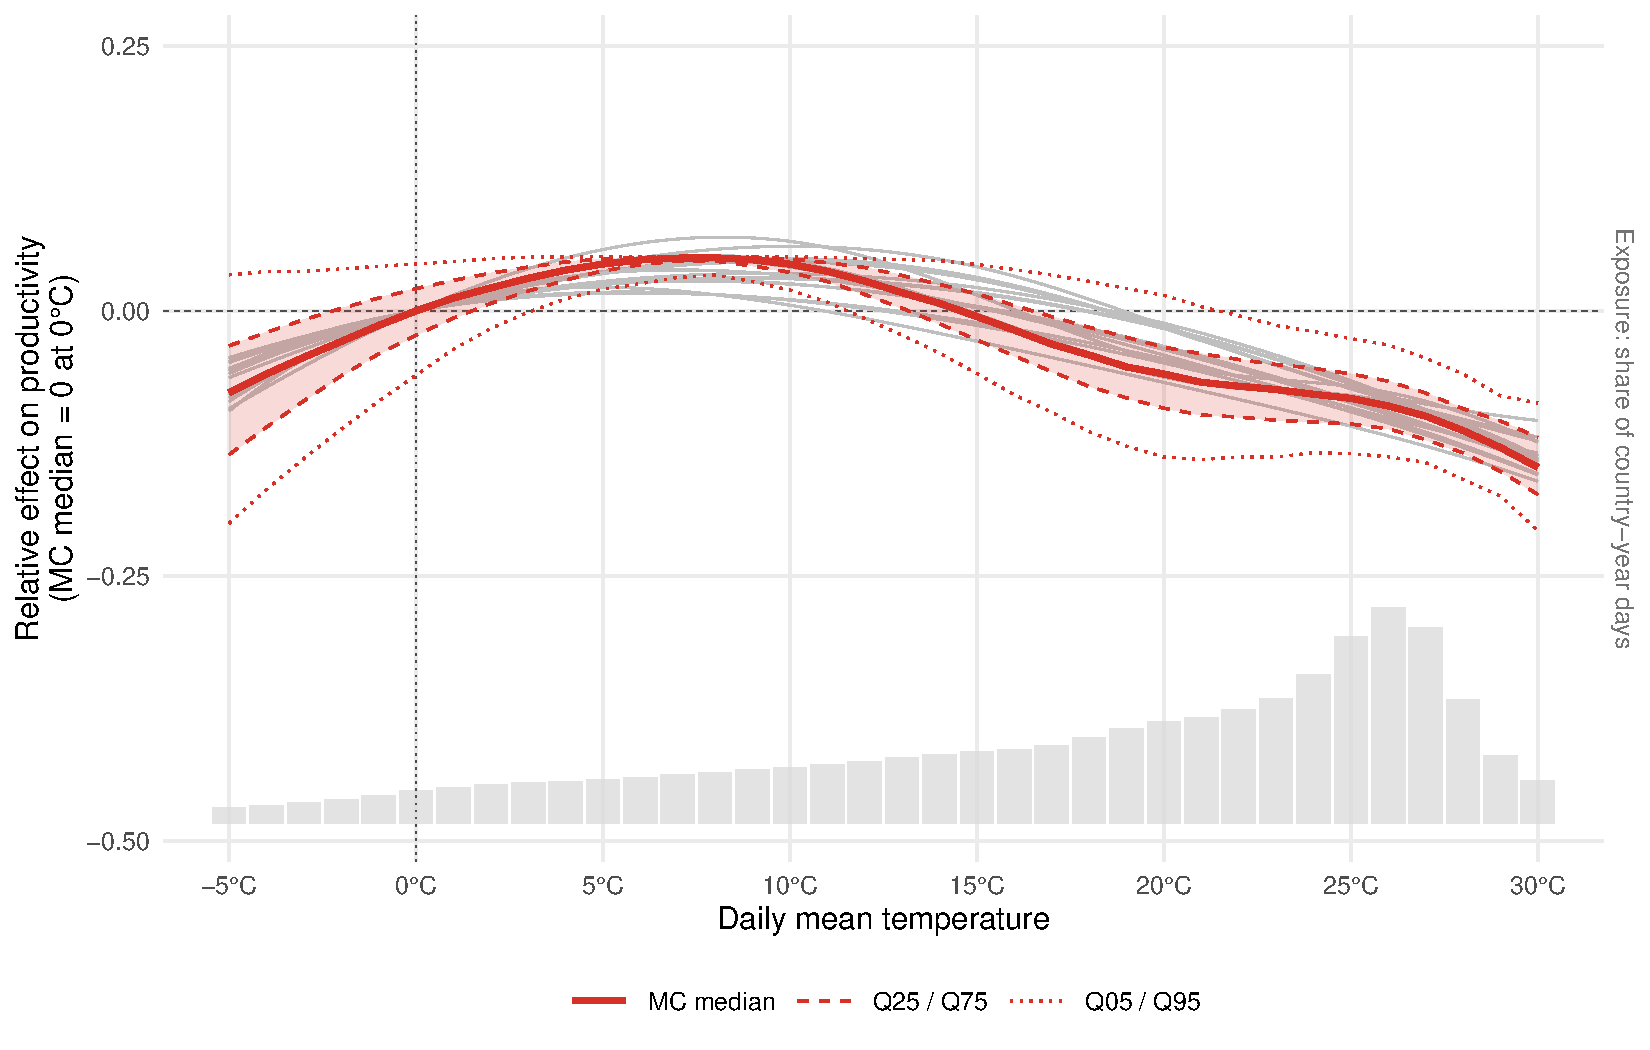
\includegraphics[width=\linewidth]{MC_prod_daily_fan_paper.pdf}\\[-2pt]
  {\small (a) Daily temperature distribution}
\end{minipage}\hfill
\begin{minipage}[t]{0.49\textwidth}
  \centering
  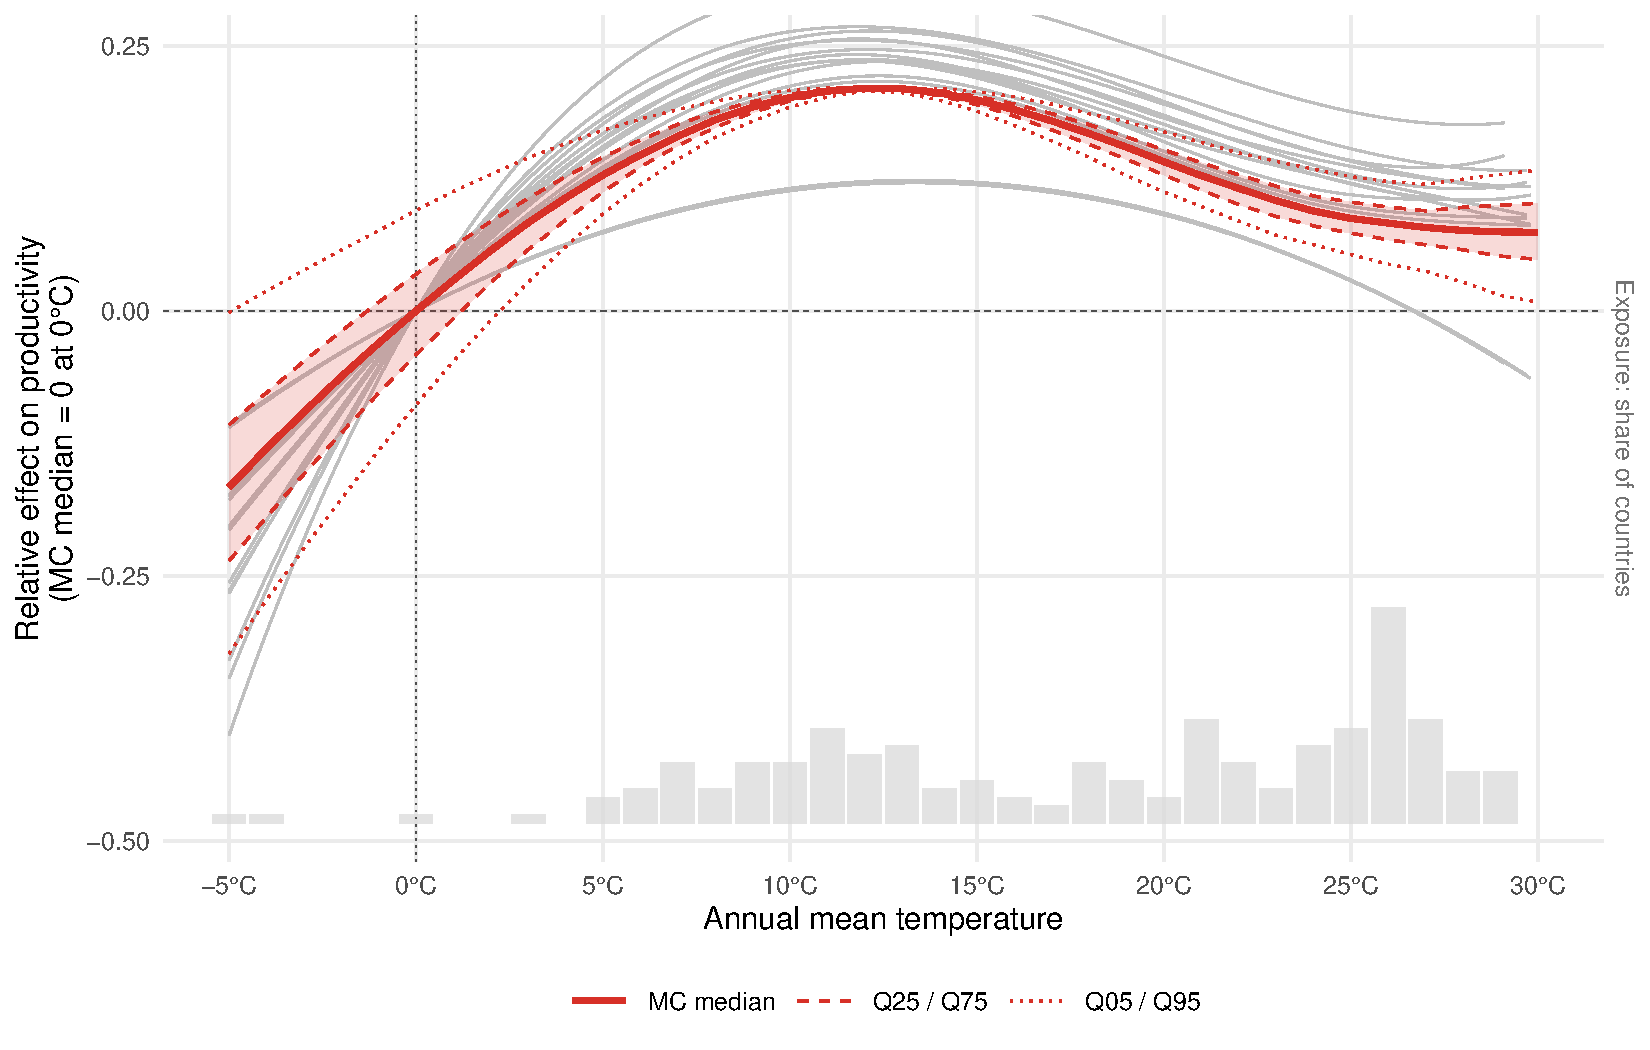
\includegraphics[width=\linewidth]{MC_prod_annual_fan_paper.pdf}\\[-2pt]
  {\small (b) Annual mean temperature}
\end{minipage}
\caption{Productivity dose-response under the two exposure metrics. Grey: the \EMPgridProdNspec{}
  specifications of the grid. Coloured: the specification carrying the Akaike weight
  (\EMPfigDrfSpecDaily{} in (a), \EMPfigDrfSpecAnnual{} in (b)), with the median, Q25--Q75 and
  Q05--Q95 of \EMPnMC{} Monte Carlo draws of its coefficients. Curves are shifted to pass
  through zero at $0^\circ$C. Bars: the arm's own exposure, share of country-year days in (a)
  and of countries in (b).}
\label{fig:drf}
\end{figure}

\subsection{Amenities are not identified from bilateral migration}
The same logic applies to amenities: the bilateral migration equation of the model, with
the pair effect absorbing fundamental amenities and migration costs, is estimated by PPML on
the \citet{abel2019bilateral} five-year flows. The temperature
terms are jointly insignificant in every cell of the amenity grid under either metric
(daily: $p=\EMPamenPjointLo$--$\EMPamenPjointHi$; annual:
$p=\EMPamenAnnualPjointLo$--$\EMPamenAnnualPjointHi$), and a placebo on lead differentials is
not rejected. That null is uninformative: the level of $f_a$ is not identified, since the pair
effect absorbs the time-invariant differential, and what survives it, the within-pair
change over five years, is too small for the test to have power against the alternatives of
interest. I therefore bound $f_a$ rather than rely on its
estimate: monotonicity and the restriction that non-market damages do not exceed market
ones give the identified set $[0,\hat f_z]$, which the migration estimate exceeds by a
factor of \EMPamenScaleExcess. The body runs the counterfactual at the lower bound,
$f_a=0$, so that welfare flows through productivity alone; Supplement~\ref{supp:ge_amenity}
re-runs it at the estimate, a stress test beyond the admissible bound, which enlarges the
global loss and deepens the Northern contrast.

\subsection{The contrast between metrics}
 \label{sec:contrast}

The two dose-responses of Figure~\ref{fig:drf} are estimated on the same
cells with the same controls, so the natural test of whether the exposure
metric matters is to project each onto the same warming and compare.
Figure~\ref{fig:contrast} does this for the productivity fundamental of the
North above $45^\circ$N. For each of the $\EMPgridProdNspec$ specifications
of the grid it reports the projected change by 2100 under
SSP2-4.5 when exposure is the annual mean, when it is the daily distribution,
and the difference between the two with its 95\% interval. Nothing is solved
in general equilibrium here: the projection integrates each estimated function against the
change in each cell's exposure, population-weighted, and isolates what the estimation
delivers before the model reallocates anything. \\
 
\begin{figure}[!ht]
\centering
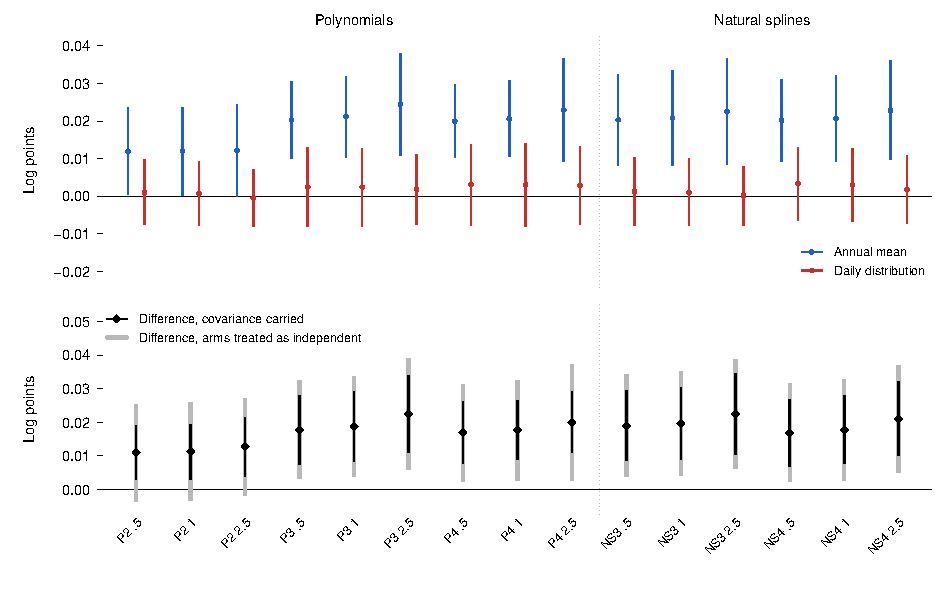
\includegraphics[width=\textwidth]{fig_contrast_grid.pdf}
\caption{Projected change in the Northern log productivity fundamental above $45^\circ$N by
  \GEhorizonLabel{} under SSP2-4.5, in partial equilibrium, for each of the \EMPgridProdNspec{}
  specifications. Top: annual mean (blue) and daily distribution (red), with 95\% intervals.
  Bottom: their difference, with the interval (clustered by origin and destination) carrying the covariance (black) or treating the arms as independent (grey).}
\label{fig:contrast}
\end{figure}

\par Three facts are read off the figure. First, in the top panel, under the
annual mean the Northern change runs from $\EMPgridAnnualMin$ to $\EMPgridAnnualMax$ log
points, and the intervals exclude zero in $\EMPgridAnnualExcl$ of the $\EMPgridProdNspec$
specifications. A literature that measures exposure by annual means will find a precise positive Northern
response under almost any form it tries.

Second, still in the top panel, under the daily
distribution the same specifications run from $\EMPgridDailyMin$ to $\EMPgridDailyMax$, with a
median of $\EMPgridDailyMedian$, with $\EMPgridDailyNneg$ below zero and none excluding
it; their intervals together span
$[\EMPgridDailyCIloMin,\EMPgridDailyCIhiMax]$. The daily arm is therefore
consistent with a Northern gain, with a Northern loss and with no response
at all, and what it establishes is that the sign of the direct Northern
response is not identified at this resolution. 

Third, in the bottom panel, the
difference between the two arms excludes zero in $\EMPdiffExcl$ of
$\EMPgridProdNspec$ specifications, which is a stronger statement than the first two would give
on their own. 

The two arms are estimated on the same
observations, and estimates drawn from the same data move together. A sample
that happens to make the annual estimate larger tends to make the daily
estimate larger as well, so that the gap between them is more stable across
samples than either level; formally, the variance of a difference subtracts
twice the covariance, and here the covariance is positive, with a
correlation between the two coefficient vectors of $\EMPdiffRhoLo$ to
$\EMPdiffRhoHi$ across the grid. Carrying that covariance, the standard error
of the difference is $\EMPdiffSEshareLo$ to $\EMPdiffSEshareHi\%$ of what it
would be if the two arms were treated as independent. Treating them as
independent therefore overstates the uncertainty of the difference, and it
is the conservative calculation: under it, the difference still excludes
zero in $\EMPdiffExclNaive$ of $\EMPgridProdNspec$ specifications, the
exceptions being \EMPdiffExclNaiveExceptions. Discounting
the covariance entirely would still find the difference signed across most of the
grid. \\


The same erosion appears in a design that shares neither the data, nor the unit, nor the
fundamental of the bilateral estimator. Supplement~\ref{supp:crh} re-runs the contrast
inside the estimation of \citet{cruz2024economic} on fundamentals inverted from their
model (a cell of one degree across four decadal cross-sections, under their
sub-region$\times$period fixed effects, their controls and their estimation sample)
using my own inversion rather than their deposited series, so that inversion, estimation
and projection stay inside one reproduction, changing only the exposure metric. Under the annual mean the projected Northern
productivity change is significantly positive in \EMPcrhSigPosAnnual{} cases out of \EMPcrhNunits{}; under
the daily distribution it is significantly positive in \EMPcrhSigPosDaily{} case out of \EMPcrhNunits{},
and for the Northern aggregate the annual-mean projection exceeds the daily one by
$\EMPcrhNorthDiff$ in the log fundamental $[\EMPcrhNorthDiffLo,\EMPcrhNorthDiffHi]$, the
daily projection being no longer distinguishable from zero. An omitted confound specific to bilateral trade cannot account for a loss of
identification in a design built on inverted cell fundamentals.
\section{General-Equilibrium Illustration}
\label{sec:ge}
Section~\ref{sec:contrast} established what the two metrics deliver before
the economy adjusts: a Northern gain under one, an unsigned response under
the other. Whether that difference survives once trade and migration
reallocate activity, and what it amounts to in welfare, is a question the
estimates cannot answer on their own. This section propagates each
dose-response through the model of Section~\ref{sec:model} along the same
emissions pathway and reports the difference.


\subsection{Scenarios and data}
\label{sec:ge_scenarios}

I simulate the model along three paths that share the same exogenous
population and productivity trajectories and differ only in climate. The
no-climate-change baseline holds exposure at its 2015 value, so that the
climate multiplier in relative changes equals one in every period; Scenario~1
applies the annual-mean pair
$(\mathcal{E}^{\text{ann}},f_z^{\text{ann}})$; Scenario~2 applies the
daily-distribution pair $(\mathcal{E}^{\text{daily}},f_z^{\text{daily}})$; a
third scenario applies the daily response to annual-mean exposure,
$(\mathcal{E}^{\text{ann}},f_z^{\text{daily}})$, and serves the decomposition of
Section~\ref{sec:ge_gap}.
The scenarios are solved on one specification per arm: for the daily response,
\EMPfigDrfSpecDaily{}; for the annual one, \EMPfigDrfSpecAnnual{}.
The reported object for a cell is the cumulative log change of period
utility relative to the baseline at 2100,
$\sum_{s\le t}\log[\dot u^{\text{scen}}_s(r)/\dot u^{\text{base}}_s(r)]$,
aggregated with population weights, and the daily extra is the
difference between the two scenarios. It is a level effect on regional utility at the horizon, not a growth effect \citep{nath2024much}. 

The grid
has $\GEncells$ inhabited $1^\circ$ cells and $\GEnperiods$ five-year
periods. Cells outside the \citet{cruz2024economic} grid, \GEdomPopOutShare\% of world population,
are excluded (Supplement~\ref{supp:calibration}). Initial trade shares come from
\citet{cruz2024economic} trade-cost matrix, initial migration shares from
\citet{abel2019bilateral} and \citet{niva2023world}, and population and
productivity paths from SSP2 \citep{kc2024updating}. Productivity growth is the average of the IAMC models available for each country under
SSP2 --- OECD Env-Growth \citep{dellink2017long}, IIASA GDP and
 PIK GDP-32 \citep{leimbach2017growth}.
Local productivity is
proxied from observed GDP per capita and set to zero in cells without positive productivity and wage or with at most
$\GEdensityCut$~\GEdensityCutUnit, so that the
model is never inverted: activity can
reallocate across inhabited cells but not into empty ones. This closes the
extensive margin of adaptation on which part of the Northern
gains rests, and it is conservative against the contrast examined here. Future temperatures are the ensemble mean of the \GEcmipModels{} CMIP6 Earth System Models
under SSP2-4.5, bias-adjusted and downscaled to $0.5^\circ$ against the W5E5 observational
dataset by ISIMIP3b \citep{lange2019trend, lange2021isimip3b}.
What the daily metric takes from them is the
distribution of daily temperatures pooled over each five-year period, which
is a climatological object rather than a weather trajectory; where regional
extremes are misrepresented, the assessed direction of the bias is an
understatement of hot extremes \citep{vautard2023heat}. \\

Every magnitude below is a difference between two scenarios run on the same
initial state, the same solver and the same iteration path. Whatever the
calibrated initial state carries enters both scenarios and cancels to first
order in the difference, and I do not report levels. The only uncertainty
propagated through the model is the Monte Carlo band on the dose-responses.

\subsection{What the metric governs}
\label{sec:ge_metric}

Table~\ref{tab:ge} reports the three margins at 2100. At the world level the
daily distribution adds losses to the annual mean rather than redistributing
them: the daily extra is $\GEworldExtra$ on top of an annual total
of $\GEworldAnnual$, and it is negative at every horizon, so that by 2100 it
adds losses equal to $\GEampRatio\%$ of the annual total. The share of the
world population living in cells that gain from warming falls from
$\GEpopGainAnnual\%$ under the annual mean to $\GEpopGainDaily\%$ under the
daily distribution.

Above $45^\circ$N the annual-mean gain of $\GEnorthAnnual$ becomes
$\GEnorthNet$. The daily extra of $\GEnorthDailyExtra$ is negative for
$\GEnorthPopLoss\%$ of the $\GEnorthPopM$~million people in that aggregate,
and in the central run the daily total is negative at every latitude
threshold of the grid, and within rounding of zero above $66.5^\circ$N,
where \GEnorthArcticPopM~million people live
(Section~\ref{sec:ge_north} reports the draws); the second line under each unit in
Table~\ref{tab:ge} shows that the loss holds across the Monte Carlo band above
$45^\circ$N and not above $66.5^\circ$N. Among the cold
economies, the annual mean projects a gain in $\GEnorthNGain$ of
$\GEnorthNcty$ and the daily extra is negative in $\GEnorthNExtraNeg$ of $\GEnorthNcty$,
so that every gain the annual mean projects is removed by the daily
distribution. What separates these economies is the size of the gain the
daily distribution removes, not whether it is removed: Russia enters with
$\GEctyRusAnnual$ and carries a daily extra of $\GEctyRusDailyExtra$, while
Germany enters with $\GEctyDeuAnnual$ and needs only $\GEctyDeuDailyExtra$.

% GENERATED by 02_GE/emit_values.py -- DO NOT EDIT BY HAND
% amenity = none
\begin{table}[!ht]
\centering
\small
\caption{General-equilibrium welfare effects by \GEhorizonLabel{}, cumulative population-weighted $\Delta\log U$, amenities at the lower bound $f_a=0$. Daily total and Annual total are each arm against the no-climate baseline; Daily extra is their difference, computed before rounding. Second line under each unit: 5th--95th percentile range and share of negative outcomes of the daily total across \GEarmBnDraws{} Monte Carlo draws of the daily dose-response, each solved in general equilibrium (Table~\ref{tab:ge_band_ranked}).}
\label{tab:ge}
\begin{tabular}{lrrr}
\toprule
& Daily total & Annual total & Daily extra \\
\midrule
\multicolumn{4}{l}{\textit{Panel A. World}} \\
World & $-0.017$ & $-0.008$ & $-0.010$ \\
\quad{\footnotesize 5th--95th pct.} & {\footnotesize [$-0.029$,\,$-0.005$]} & \multicolumn{2}{l}{\footnotesize negative in 60 of 60 draws} \\
\addlinespace
\multicolumn{4}{l}{\textit{Panel B. By latitude}} \\
$\geq 45^\circ$N & $-0.006$ & $+0.011$ & $-0.018$ \\
\quad{\footnotesize 5th--95th pct.} & {\footnotesize [$-0.011$,\,$-0.003$]} & \multicolumn{2}{l}{\footnotesize negative in 60 of 60 draws} \\
$\geq 55^\circ$N & $-0.003$ & $+0.023$ & $-0.027$ \\
\quad{\footnotesize 5th--95th pct.} & {\footnotesize [$-0.008$,\,$+0.0002$]} & \multicolumn{2}{l}{\footnotesize negative in 56 of 60 draws} \\
$\geq 66.5^\circ$N & $0.000$ & $+0.033$ & $-0.033$ \\
\quad{\footnotesize 5th--95th pct.} & {\footnotesize [$-0.005$,\,$+0.004$]} & \multicolumn{2}{l}{\footnotesize negative in 29 of 60 draws} \\
\addlinespace
\multicolumn{4}{l}{\textit{Panel C. Cold-climate economies}} \\
Russia & $-0.003$ & $+0.025$ & $-0.028$ \\
\quad{\footnotesize 5th--95th pct.} & {\footnotesize [$-0.008$,\,$+0.0004$]} & \multicolumn{2}{l}{\footnotesize negative in 55 of 60 draws} \\
Finland & $-0.001$ & $+0.027$ & $-0.028$ \\
\quad{\footnotesize 5th--95th pct.} & {\footnotesize [$-0.006$,\,$+0.004$]} & \multicolumn{2}{l}{\footnotesize negative in 38 of 60 draws} \\
Norway & $-0.005$ & $+0.013$ & $-0.018$ \\
\quad{\footnotesize 5th--95th pct.} & {\footnotesize [$-0.009$,\,$-0.001$]} & \multicolumn{2}{l}{\footnotesize negative in 59 of 60 draws} \\
Sweden & $-0.004$ & $+0.012$ & $-0.017$ \\
\quad{\footnotesize 5th--95th pct.} & {\footnotesize [$-0.009$,\,$-0.0002$]} & \multicolumn{2}{l}{\footnotesize negative in 57 of 60 draws} \\
Canada & $-0.010$ & $+0.011$ & $-0.021$ \\
\quad{\footnotesize 5th--95th pct.} & {\footnotesize [$-0.016$,\,$-0.004$]} & \multicolumn{2}{l}{\footnotesize negative in 60 of 60 draws} \\
Germany & $-0.007$ & $+0.004$ & $-0.011$ \\
\quad{\footnotesize 5th--95th pct.} & {\footnotesize [$-0.011$,\,$-0.003$]} & \multicolumn{2}{l}{\footnotesize negative in 60 of 60 draws} \\
France & $-0.012$ & $-0.008$ & $-0.004$ \\
\quad{\footnotesize 5th--95th pct.} & {\footnotesize [$-0.017$,\,$-0.008$]} & \multicolumn{2}{l}{\footnotesize negative in 60 of 60 draws} \\
\addlinespace
Population in gaining cells (\%) & 0.1 & 11.7 & --- \\
\bottomrule
\end{tabular}
\end{table}




Figure~\ref{fig:ge_maps} shows the geography: the annual-mean panel's beneficiaries are
among the daily-total panel's losers, and the daily extra is deepest where the annual-mean
gain is largest.

\begin{figure}[!ht]
\centering
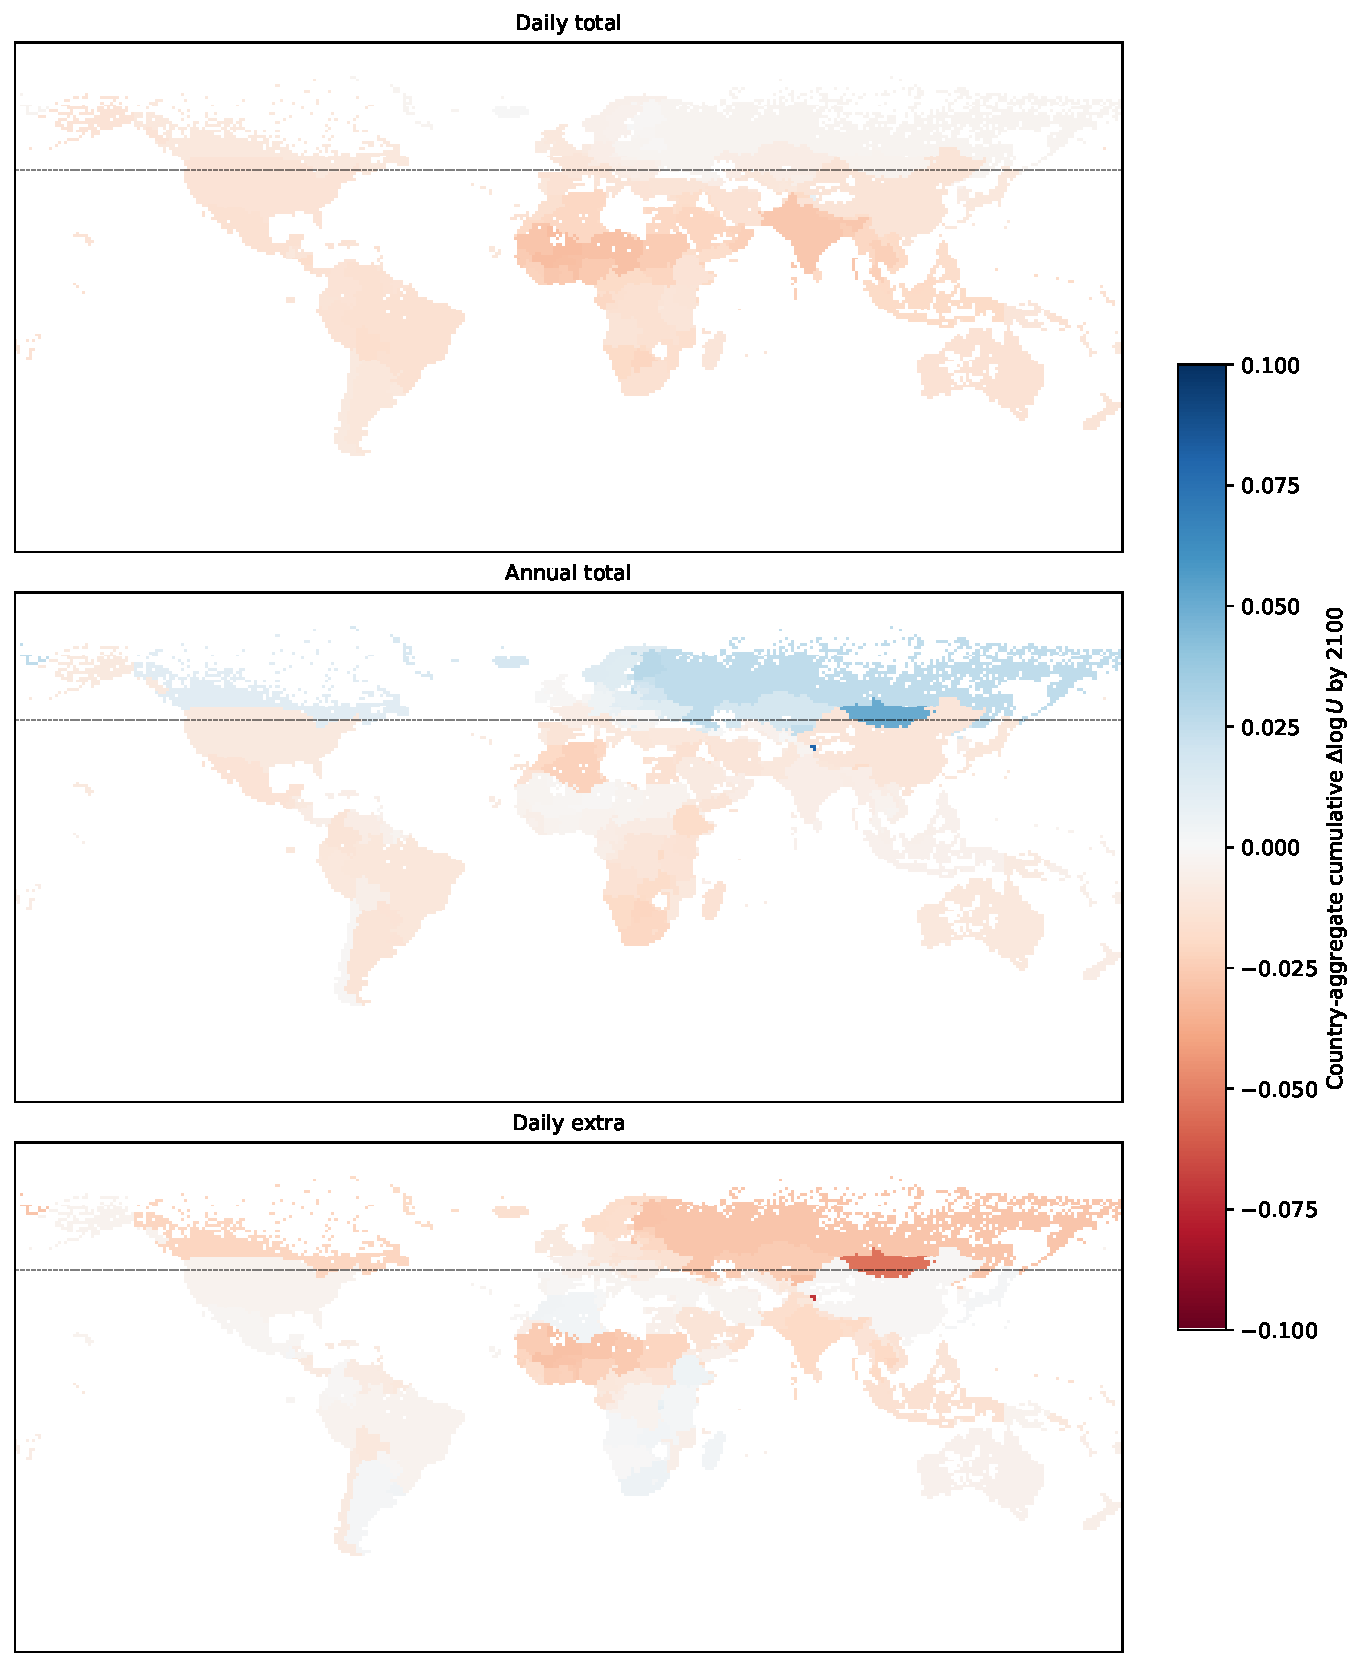
\includegraphics[width=\textwidth]{map_welfare_2100_country.pdf}
\caption{The three maps show the country-aggregate, population-weighted
  cumulative $\Delta\log U$ by \GEhorizonLabel\  under the daily total, the annual total
  and the daily extra, with amenities at the lower bound. The colour scale is
  common to the three panels and centred at zero.}
\label{fig:ge_maps}
\end{figure}


\newpage 

\par Figure~\ref{fig:ge_tiers} reports the three margins by population-weighted
quartile of 1990 GDP per capita. The daily total loads heaviest on the poorest
quartile (\GEtierQoneDaily{} against \GEtierQfourDaily{} in the richest) but aggregating exposure
understates damages at both ends of the income distribution: in the poor hot
economies through the hot tail, and in the rich cold ones through the removal
of the annual-mean gain. The band on the daily total is negative at every
quartile.

\begin{figure}[!ht]
\centering
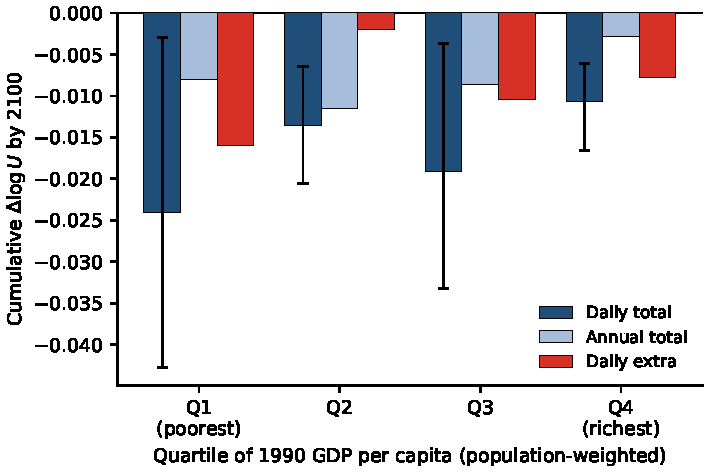
\includegraphics[width=0.8\textwidth]{fig_ge_tiers.pdf}
\caption{Welfare effects by \GEhorizonLabel{} by quartile of 1990 GDP per capita
  (population-weighted), cumulative $\Delta\log U$, amenities at the lower bound. Bars: daily
  total, annual total, daily extra; segments on the daily total: 5th--95th percentile range
  across \GEarmBnDraws{} Monte Carlo draws of the daily dose-response solved in general
  equilibrium.}
\label{fig:ge_tiers}
\end{figure}

\subsection{Where the gap comes from}
\label{sec:ge_gap}

The two scenarios compute different objects. Scenario~1 evaluates a function
estimated on annual means at the cell's annual mean,
$f_z^{\text{ann}}(\bar T)$, Scenario~2 a function estimated on
daily bins over the distribution the cell experiences,
$\int f_z^{\text{daily}}\,dF$. Their difference separates into two terms,
\[
\underbrace{f_z^{\text{ann}}(\bar T)-f_z^{\text{daily}}(\bar T)}_{\text{different function}}
\;+\;
\underbrace{f_z^{\text{daily}}(\bar T)-\int f_z^{\text{daily}}\,dF}_{\text{different evaluation}} .
\]
The second term is Jensen's inequality, which evaluates one function at a
point rather than integrating it. The first term compares two different
functions at the same argument, and it is what aggregating exposure before
estimating produces. The third scenario, $(\mathcal{E}^{\text{ann}},f_z^{\text{daily}})$,
holds the function fixed and changes only the evaluation. At the Northern
aggregate, of a daily extra of $\GEnorthDailyExtra$, the evaluation term
contributes $\GEnorthChanEval$ and the function term $\GEnorthChanShape$. The
Jensen term is \GEnorthChanSameSign\ and $\GEnorthChanRatio$ times smaller in
absolute value than the function term. The mechanism is that the
annual-mean function assigns to a warming cold country a benefit that the
daily function does not find in the same country's record. Finland's
population-weighted mean rises from $\EMPfinTmeanBase$ to
$\EMPfinTmeanProj^\circ$C by \GEhorizonLabel; the annual function returns a
productivity gain of $\EMPfinGainAnnual$ in log productivity and the daily
function
$\EMPfinGainDaily$: both functions leave Finland better off, and they disagree
by a factor of $\EMPfinGainFactor$ on how much. The country still spends
$\EMPfinDaysColdProj$ days a
year below $-10^\circ$C at the end of the projection and its days above
$25^\circ$C rise from $\EMPfinDaysVHotBase$ to $\EMPfinDaysVHotProj$. Neither
tail is visible at the mean. 

Put plainly, warming a cold country removes freezing days and adds hot days,
and a regression on days finds both to be costly. What it does not find is the
value the annual mean places on the freezing days: over the cold range the
annual-mean function values the same loss of cold days at least
\EMPgapColdRatioFloor{} times what a regression on days values it at. Measured
by the annual mean, the same country simply becomes a warmer country, and is
credited with whatever a warmer mean has been worth in the data: across
countries or across cells, the income gap between cold and temperate ones; across
years, a milder winter in the same place. These are the two sources of variation an
annual-mean regression can use. The estimator of
Section~\ref{sec:identification} uses the first across countries; the design of
Supplement~\ref{supp:crh} uses it across cells within a sub-region and period, with
\EMPcrhWithinCellTmeanProd\% of the identifying variance of the mean temperature lying
within cells across periods; and the Northern gain erodes under both. The second source is
the one panel designs use, and the one \citet{jones2026binning} show to carry
warming-induced trends (Supplement~\ref{supp:binning}). That credit is not
the price of any particular day, and a regression on days cannot reproduce it.

The gap can also be located on the temperature support without solving the
model. Integrating each estimated function against the change in each
Northern cell's daily exposure and attributing the difference to the
temperature bins in which it arises, \EMPgapShareOfContrast\% of the
Northern contrast comes from the two functions differing at the same
temperature rather than from the two metrics integrating against different
objects; of that share, \EMPgapShareBelowZero\% lies below $0^\circ$C and
\EMPgapShareAboveTwenty\% above $20^\circ$C. The two functions disagree about
the value of the freezing days that warming removes, and they agree about the
cost of the hot days it adds. The two shares are not comparable: the
general-equilibrium split divides a propagated welfare difference, the local
one divides the partial-equilibrium contrast of the estimated functions.

\subsection{Why the Northern gain does not survive equilibrium}
\label{sec:ge_north}

The daily metric does not sign the Northern response in partial
equilibrium. The equilibrium loss above $45^\circ$N is nonetheless not a coin
flip, because the Northern daily total also carries what warming elsewhere
does to the North. Two further pairs of runs measure this: in the first,
warming outside the North is switched off and only the cells at or above
$45^\circ$N warm; in the second, warming is applied only outside the North
(Supplement~\ref{supp:exposure_masks}). Warming outside the North accounts for
$\GEmaskNonNorthWarmingDailyShare\%$ of the Northern daily total. Warming in
the North alone changes Northern welfare by $\GEmaskNorthWarmingAnnual$ under
the annual-mean function and by $\GEmaskNorthWarmingDaily$ under the daily
one, so the reversal of sign happens with warming confined to the North.
What warming elsewhere does to the North is nearly the same under the two
functions and largely cancels in the daily extra: with warming confined to
the North, the Northern daily extra is $\GEmaskNorthWarmingExtraShare\%$ of its
value when the whole world warms, and warming outside the North accounts for
$\GEmaskNonNorthWarmingExtraShare\%$. 

What the daily distribution adds is an income loss that grows with latitude. Net of the amenity term, which moves only through congestion at $f_a=0$,
the daily extra is $\GEchanIncomeMid$ in the temperate band,
$\GEchanIncomeSub$ between $45$ and $60^\circ$N and $\GEchanIncomeArc$
above $60^\circ$N (Table~\ref{tab:ge_decomp_lat}).
Nearly all of it is produced by warming in the North itself rather than imported from
elsewhere, and it comes from the central draw of the dose-response.

Across $\GEarmBnDraws$ Monte Carlo draws of the
daily dose-response, each propagated through the model, the Northern daily
total is negative in \GEnorthDailyShareNeg{} draws, with a median of
$\GEnorthDailyRqMed$ and a 5th--95th percentile range of $\GEnorthDailyRqLo$
to $\GEnorthDailyRqHi$ (Table~\ref{tab:ge}). The loss is a property of the
Northern aggregate rather than of its coldest members: above $66.5^\circ$N the
daily total is negative in \GEshareNegNorthArctic{} draws, and for Finland
in \GEshareNegFin{}, so that the sign of the far North is not determined at
daily resolution, in general equilibrium as in the estimation.



\section{Conclusion}
\label{sec:conclusion}
 
There are many reasons to expect climate change to be costly in the North,
for instance biodiversity collapse, permafrost thaw under roads, pipelines and buildings, or boreal
wildfires. This paper has set those channels aside and asked a narrower
question, about the one channel the spatial models of climate damages do
quantify, the effect of temperature.

Spatial models of climate damages project welfare gains for the world's
cold economies. This paper has argued that those gains are a property of the
exposure metric. Estimated on the same data with the annual mean and with the
distribution of daily temperatures, the productivity response projects a
precise Northern gain under the first and a change centred on zero under the
second, and the difference between the two is signed in every specification
of the grid; propagated through a spatial equilibrium model of trade and
migration, the annual-mean gain of the population above $45^\circ$N becomes
a loss, and the share of the world population living in cells that gain from
warming falls from $\GEpopGainAnnual\%$ to $\GEpopGainDaily\%$. The reason is
not that a non-linear function is evaluated at the wrong point. It is that
aggregating exposure before estimating recovers a different function, one
that absorbs everything separating cold countries from hot ones and assigns
to the freezing days that warming removes a value that a function estimated
on days does not find. This is a statement about the productivity response, not about daily
resolution as such: where the cold arm of the dose-response is real, as for mortality,
daily-resolution estimates project gains for cold regions \citep{carleton2022valuing}, and
nothing here contradicts them. What the annual mean does to productivity is to manufacture a
cold arm the daily data do not support; what \citet{jones2026binning} show for panels is that
extreme-day counts can manufacture one too.
 
The exercise takes the emissions pathway as given, and the limit is a
missing object rather than a conceptual one. The emulators embedded in models
with endogenous emissions map cumulative emissions to pattern-scaled regional
annual means and produce nothing at the daily resolution on which welfare
depends. Emulators at monthly resolution now exist \citep{nath2022mesmer},
and they recover the seasonal amplitude that annual means discard; the object
this paper requires is one step further, a reduced form from cumulative
emissions to the shape of the regional daily distribution. Until it exists,
endogenous-climate and distributional-climate analyses sit on separate
branches of the literature, and this paper establishes what the choice
between them costs: the branch that buys endogenous emissions at the price of
the annual mean buys it at the price of the sign.
 
%TC:ignore

\begin{spacing}{1}

%% ================================================================
%  References
%% ================================================================
\bibliographystyle{chicago}
\bibliography{References_JMP}

\end{spacing}

\newpage 
%% ================================================================
%  Appendix
%% ================================================================
\appendix

\noindent

\section*{Appendix}
Supplement~\ref{supp:calibration}
documents the calibration of the initial equilibrium and the climate inputs.
Supplements~\ref{supp:productivity} and~\ref{supp:amenity} each treat one
estimated dose-response function end to end.
Supplement~\ref{supp:ge} reports the general-equilibrium detail. A final section \ref{supp:crh} sets the same question in an independent design \citep{cruz2024economic}.
\section{Calibration and Climate Inputs}
\label{supp:calibration}
%% ================================================================

The counterfactual evaluates damages along an exogenous emissions path; it
does not optimise emissions. Its calibration targets a 2015 initial state in
levels and geography from published sources, and lets the dynamics run in
relative changes from there. This section documents the initial state, the
reason the model is not inverted, and what is taken from the climate
projections.

\subsection{Data} 
The world is discretised on a $1^\circ$ grid of $\GEncellsPotential$
potential cells, of which $\GEncells$ have positive productivity, positive
wage and population above one; the rest (oceans, deserts, ice) carry no
economic content. \GEdomCellsOut{} further inhabited cells, holding \GEdomPopOutM{} million people or
\GEdomPopOutShare\% of world population, lie outside the \citet{cruz2024economic} grid:
\GEdomCtyOutN{} countries and territories, \GEdomCtyOutPopM{} million people in all, are
outside it entirely, and \GEdomCtyPartialN{} countries in part. The \GEdomMigLostM{}
million international migrants of the 2010--2015 window whose origin or destination is one
of these cells are dropped with them. Cells are mapped to countries through GHSL population
shares within GADM polygons. The
$1^\circ$ resolution is that of the \citet{cruz2024economic} trade-cost
matrix.
Fundamental productivity is proxied by GDP per capita
\citep[gridded GDP from][GHSL population, 2015]{kummu2025gdp},
winsorised at the upper $5\%$ tail; the wage is that proxy times the ILO 2015
country labour share (regional imputation, then global mean, where missing).
Initial trade shares follow $\lambda_0(rs)\propto Z(s)^{\theta}\,w(s)^{-\alpha\theta}
\tau_{rs}^{-\theta}$ with $\theta=\GEtheta$ \citep{desmet2018geography} and
$\alpha=0.6$ \citep{desmet2015spatial}, and the \citet{cruz2024economic}
cost matrix,
rows summing to one over sources. At $\approx$100~km resolution this grid is
close to autarky: $\GElamDiagShareHigh\%$ of cells spend more than $0.99$ of
their income on their own output, and the mean import share is
$\GEimportShareMean\%$. GDP per capita is not an Eaton--Kortum
fundamental, so the raw allocation $(Z,w,L,\tau)$ need not clear exactly.
Because the model is solved in relative changes, only $\lambda_0$ enters, and
any residual adjustment transient is common to the three scenarios and
differences out of every reported contrast. 

The five-year transition matrix $\mu_0$ combines international bilateral
flows from \citet{abel2019bilateral} (2010--2015), allocated to cells by
within-country population shares, and internal flows reconstructed from the
\citet{niva2023world} net migration stocks (2010--2014) by an outer product of origin and destination shares. Within each country, internal flows
are allocated across the cells in which it holds at least half of the population, origins
weighted by the country's population in the cell and destinations by the positive part of
the net migration stock that the international flows leave there; the cross-border mass
this leaves is \GEmigInternalCrossM{} million over the window,
\GEmigInternalCrossShare\% of the internal block. Diagonals are zeroed,
stayers added, rows normalised to transition probabilities, flows capped by
population. Three limitations: the within-country allocation assumes no
sub-national distance friction; the internal gross structure is
reconstructed from net stocks, not observed; and the same matrix is applied
at each of the $\GEntransitions$ transitions, so that the refugee-driven flows
of the 2010--2015 window (Pakistan, Afghanistan, Syria) recur throughout.
Figure~\ref{fig:mig_latitude} shows net losses from the tropics to about
$35^\circ$N and net gains over the temperate belt.

\begin{figure}[H]
\centering
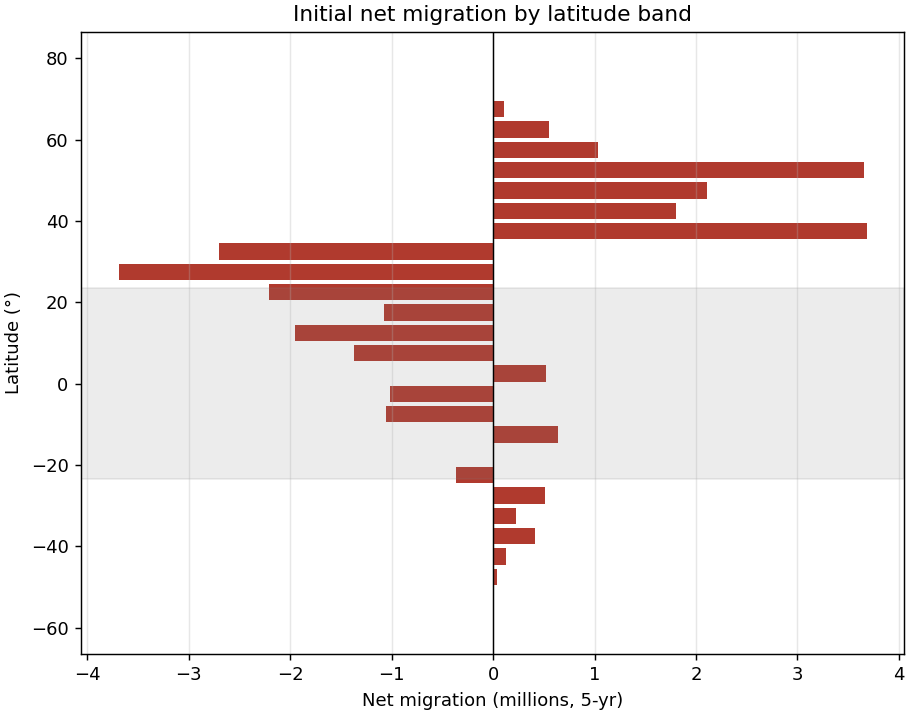
\includegraphics[width=0.7\textwidth]{fig_M1_net_by_latitude.png}
\caption{Net migration by latitude from the calibrated initial matrix.}
\label{fig:mig_latitude}
\end{figure}

Spatial models of climate damages recover unobserved fundamentals by
inverting the model on an observed equilibrium. The inversion assigns a
positive fundamental to every cell, including empty ones, so that under
warming activity can relocate into them and the gain is counted as
adaptation. This extensive margin is part of what generates the Northern
gains in that literature, and two facts argue against relying on it.
Observed international net migration over 1990--2020, a period of roughly
$0.6^\circ$C of warming, shows no clear accelerating northward trend
(Figure~\ref{fig:migration}): legal barriers, income gaps and networks have
dominated the climate signal at these horizons
\citep{cattaneo2019human}. And the cells into which
the inverted margin routes activity are largely cells with no activity today
(Figure~\ref{fig:activity_map}); their emptiness has causes (institutions,
infrastructure, property rights, labour markets) that warming does not
remove. I therefore proxy productivity from observed data, set it to zero
in cells without positive productivity and wage or with at most $\GEdensityCut$~\GEdensityCutUnit,
and let adaptation run only on
the intensive margins the data record. Re-opening the extensive margin
would add cold high-latitude destinations for displaced activity, and so
amplify the annual-mean Northern gain; the restriction is conservative
against the contrast the paper examines.

\begin{figure}[H]
\centering
\centerline{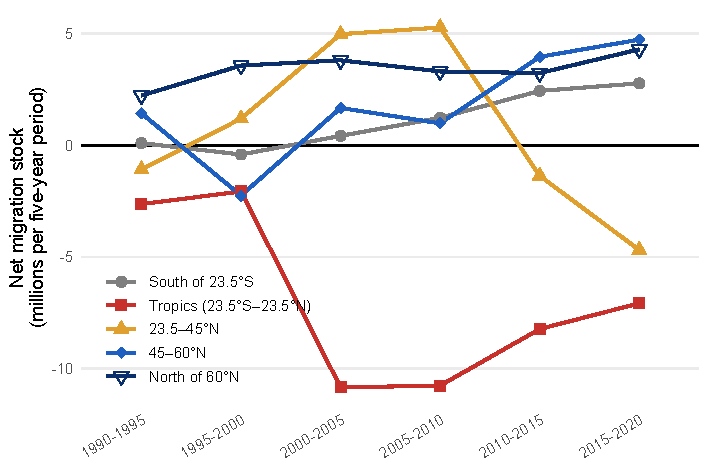
\includegraphics[width=0.8\textwidth]{myplot_migration.pdf}}
\caption{Net international migration stock by latitude band and five-year
  period, 1990--2020, from \citet{abel2019bilateral}. Countries are assigned
  to bands by the latitude of their centroid; the five bands sum to zero in
  each period.}
\label{fig:migration}
\end{figure}

\begin{figure}[H]
\centering
\centerline{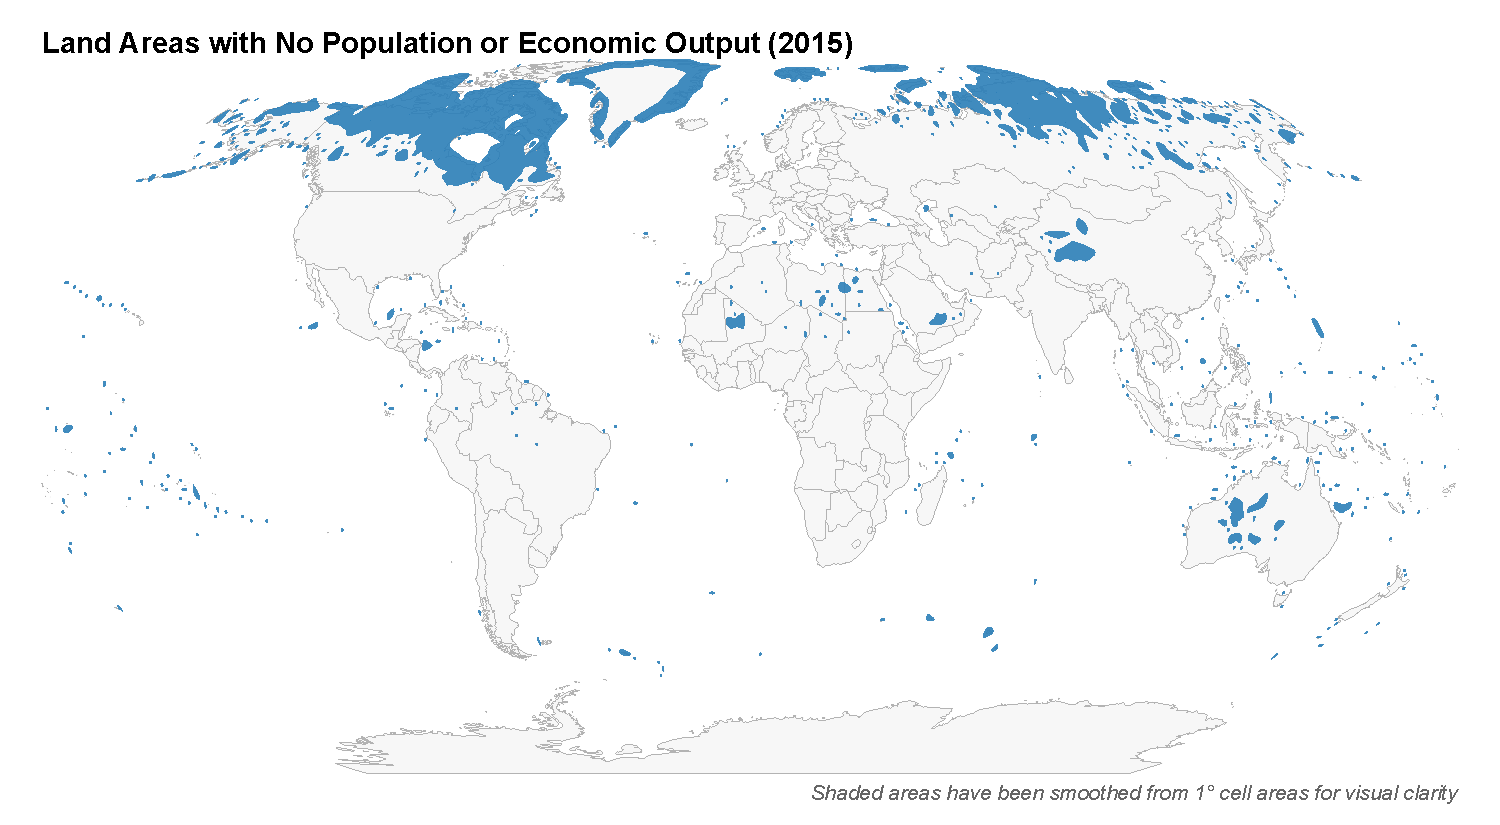
\includegraphics[width=0.9\textwidth]{no_activity_map_smooth_light.pdf}}
\caption{Areas of zero recorded economic activity in 2015 (blue). Model
  inversion assigns positive fundamental productivity to these cells.}
\label{fig:activity_map}
\end{figure}

\subsection{Model: equilibrium conditions}
\label{supp:model_equilibrium}

Workers are freely mobile at a bilateral cost. A worker in $s$ who locates
in $r$ obtains $u_t(r)\,m(sr)^{-1}\epsilon$, where $u_t(r)=a_t(r)\,y_t(r)$
is spatial welfare, $y_t(r)$ real income per capita, $m(sr)$ a
time-invariant and symmetric migration cost, and $\epsilon$ an i.i.d.
Fr\'echet shock with dispersion $\Omega$; symmetry makes the location
problem static \citep{desmet2018geography}. The share of population of
$s$ that locates in $r$ is
\begin{equation}
\mu_t(sr)=\frac{\bigl[u_t(r)/m(sr)\bigr]^{1/\Omega}}
              {\sum_{n}\bigl[u_t(n)/m(sn)\bigr]^{1/\Omega}},
\label{eq:mu}
\end{equation}
and population evolves with exogenous births and deaths and these flows.
Each cell produces a continuum of varieties under perfect competition with
labour and structures, with a labour share $\alpha$ and productivity draws
from a Fr\'echet distribution of scale $Z_t(r)^{\theta}$ and shape $\theta$; goods
are traded at iceberg costs $\tau_{sr}$ with balanced trade. With $x_t(r)$
the unit cost of the input bundle, the share of $r$'s expenditure on goods
from $s$ and the price index are
\begin{equation}
\lambda_t(rs)=\frac{Z_t(s)^{\theta}\bigl(x_t(s)\tau_{sr}\bigr)^{-\theta}}
                    {\sum_{l}Z_t(l)^{\theta}\bigl(x_t(l)\tau_{lr}\bigr)^{-\theta}},
\qquad
P_t(r)=\Gamma\Bigl[\sum_{s}Z_t(s)^{\theta}\bigl(x_t(s)\tau_{sr}\bigr)^{-\theta}\Bigr]^{-1/\theta}.
\label{eq:trade}
\end{equation}
Rents on structures accrue to local residents, so that income per capita
is $w_t(r)/\alpha$ and real income is $y_t(r)=w_t(r)/(\alpha P_t(r))$; the
goods market clears when $w_t(r)L_t(r)=\sum_s\lambda_t(sr)\,w_t(s)L_t(s)$.

The model is solved in relative changes, $\dot x_{t+1}=x_{t+1}/x_t$. Because
migration costs and structures are time-invariant, the system
\eqref{eq:mu}--\eqref{eq:trade} in changes involves only the observed
shares of the previous period, the elasticities, and the changes in
fundamentals implied by \eqref{eq:channels}:
\begin{equation}
\dot\mu_{t+1}(sr)=\frac{\dot u_{t+1}(r)^{1/\Omega}}
   {\sum_{n}\mu_t(sn)\,\dot u_{t+1}(n)^{1/\Omega}},
\qquad
\dot P_{t+1}(r)=\Bigl[\sum_{s}\lambda_t(rs)\,\dot Z_{t+1}(s)^{\theta}\,
   \dot x_{t+1}(s)^{-\theta}\Bigr]^{-1/\theta},
\label{eq:hat}
\end{equation}
with $\dot Z_{t+1}(r)=\gamma_{t+1}(r)\exp[\mathcal{E}_{t+1}(r)f_z-\mathcal{E}_t(r)f_z]$
for exogenous growth $\gamma$, and
for fundamental amenities, $\dot a_{t+1}(r)=\dot L_{t+1}(r)^{-\lambda}\exp[\mathcal{E}_{t+1}(r)f_a-\mathcal{E}_t(r)f_a]$;
the changes in trade shares, wages and utility follow from \eqref{eq:trade},
market clearing and $\dot u=\dot a\,\dot y$. Each transition is solved as a
fixed point on next-period population, with a nested fixed point on wages
and trade shares.
Unobserved fundamentals $\bar Z$ and $\bar a$ and costs $m$ and $\tau$ enter
only through the observed initial shares $\lambda_0$ and $\mu_0$; they are
never recovered by inversion. That choice closes the extensive margin of
adaptation: a cell with no observed activity has no share to scale, and no
counterfactual can route activity into it.






%% ================================================================
\section{The Productivity Dose-Response}
\label{supp:productivity}
%% ================================================================

This section collects the evidence behind the productivity dose-response of
the body: the sample and first stage, the identification argument and its
tests, the robustness of the estimated function across specifications, and the
contrast between the two exposure metrics across the same grid.

%% ----------------------------------------------------------------
\subsection{Sample and first stage}
\label{supp:prod_sample}
%% ----------------------------------------------------------------

The estimation combines BACI--CEPII bilateral trade flows (1995--2019) with
GLORIA input--output tables for domestic absorption, World Bank GDP per
capita, and ERA5 temperatures \citep{hersbach2020era5} aggregated to countries
with GHSL-POP population weights. Daily means are computed by the data provider over the UTC calendar day from hourly
fields, so that for cells far from the Greenwich meridian the day boundary falls within
local daytime. Three exclusions reduce the ISIC Rev.3
nomenclature to $\EMPtradeNsectors$ manufacturing and agricultural sectors:
primary and extractive industries (divisions 02, 05, 10--14), whose
productivity is driven by endowments and whose domestic absorption is near
zero, which destabilises the normalisation; services (divisions 40 and above),
for which $X^k(rs)/X^k(rr)$ is not defined in the GLORIA final-demand matrix;
and divisions 18, 30 and 33, recorded by BACI but absent from GLORIA. A
fourth exclusion follows from the sectoral elasticities: division 99, goods
not elsewhere classified, which the concordance populates almost entirely
with waste, scrap and used goods, has no elasticity in
\citet{caliendo2015estimates} and is dropped. Divisions 18, 30 and 33 carry
$\EMPtradeGloriaLossObs\%$ of trade lines and $\EMPtradeGloriaLossVal\%$
of trade by value, measured on the product-level BACI lines that remain once
division 99 and non-country entities are removed, and
$\EMPtradeGloriaLossPairs$ country pairs lose complete year coverage. Before the exclusions the sample has
$\EMPtradeNobs$ observations; $\EMPtradeNoClimObs$ of them belong to pairs involving one of
\EMPtradeNoClimCountries{} countries without an ERA5 record and are dropped, and the sample on
which the dose-responses are estimated has $\EMPtradeNobsStageThree$. Bilateral trade costs are unobserved and proxied by the gravity vector
$C_{rs}$: log distance, common official language, colonial link, and a WTO
free-trade-agreement indicator. A spline's interior knots sit at equally spaced quantiles of the exposure
distribution its arm uses (the day-weighted distribution of daily means
under one metric, the distribution of annual means under the other) and its
boundary knots at the winsorisation thresholds. Monte Carlo draws are
$\boldsymbol\beta^{(b)}\sim\mathcal N(\hat{\boldsymbol\beta},\hat\Sigma)$; the joint and non-linearity tests across this grid
are in Supplement~\ref{supp:prod_robustness}.


%% ----------------------------------------------------------------
\subsection{Identification}
\label{supp:prod_identification}
%% ----------------------------------------------------------------

\paragraph{Between-pair variation.}
Table~\ref{tab:fe_absorption} quantifies the statement of the body that
bilateral temperature differentials are quasi-permanent:
origin$\times$destination$\times$product effects absorb
$\EMPfeAbsorptionMin$--$\EMPfeAbsorptionMax\%$ of the variance of the climate
terms $\Delta_k$, and the within-pair standard deviation of $\Delta_k$ is at
most $\EMPwithinPairSDMax\%$ of its total. Product$\times$year effects absorb
at most $\EMPprodYearAbsorpMax\%$. Table~\ref{tab:ctrl_absorption} shows what
the gravity controls do against the remaining between-pair variation: they
absorb $\EMPctrlAbsorpLo$--$\EMPctrlAbsorpHi\%$ of it, conditional on
product$\times$year effects, without being collinear with the climate term.

%% GENERATED by 01a_productivity_drf.R -- DO NOT EDIT BY HAND.
\begin{table}[H]
\centering\small
\caption{Variance absorption by fixed effects}
\label{tab:fe_absorption}
\begin{tabular}{lccc}
\hline\hline
Climate term & Pair$\times$prod FE & Prod$\times$year FE & Both FE \\
\hline
$\Delta_1$ & 0.9969 & 0.004125 & 0.9969 \\
$\Delta_2$ & 0.9942 & 0.002871 & 0.9942 \\
$\Delta_3$ & 0.9768 & 0.003096 & 0.9769 \\
\hline\hline
\multicolumn{4}{p{\dimexpr\linewidth-2\tabcolsep\relax}}{\footnotesize
$R^2$ from projecting the bilateral climate differential
$\Delta_k = g_k(T(s)) - g_k(T(r))$ on fixed effects alone (OLS).
Origin$\times$destination$\times$product fixed effects absorb
at least 97.7\% of the variance in bilateral climate differentials
(97.7\%--99.7\% across the three terms), leaving insufficient
residual variation for PPML identification.
Product$\times$year fixed effects absorb at most 0.41\%,
preserving the between-pair variation that identifies $g(\cdot)$.}
\end{tabular}
\end{table}

%% GENERATED by 01a_productivity_drf.R -- DO NOT EDIT BY HAND.
\begin{table}[H]
\centering\small
\caption{Absorption of between-pair confounders by gravity controls}
\label{tab:ctrl_absorption}
\begin{tabular}{lccc}
\hline\hline
Climate term & $R^2$ (FE only) & $R^2$ (FE + controls) & Absorbed \\
\hline
$\Delta_1$ & 0.004125 & 0.1498 & 0.1456 \\
$\Delta_2$ & 0.002871 & 0.1415 & 0.1386 \\
$\Delta_3$ & 0.003096 & 0.0523 & 0.0492 \\
\hline\hline
\multicolumn{4}{p{\dimexpr\linewidth-2\tabcolsep\relax}}{\footnotesize
OLS projection of $\Delta_k$ on gravity controls conditional on
product$\times$year fixed effects. Gravity controls (log bilateral distance,
common language, colonial link, WTO FTA, $\theta^k\cdot\log(y_s/y_r)$)
absorb 4.9--14.6\% of the between-pair climate variation,
partially controlling for the main observable confounders.}
\end{tabular}
\end{table}


\paragraph{Selection on unobservables.}
Table~\ref{tab:oster_delta} reports the \citet{oster2019unobservable}
selection ratio $\delta^*$ across the specification grid, with the first-basis
coefficient without and with gravity controls. Because $\delta^*$ scales with
the inverse of the coefficient's movement, specifications whose coefficient
barely moves produce arbitrarily large values of uninformative sign; the
informative entry is the least favourable entry on the grid,
$\delta^*=\EMPosterDelta$,
whose coefficient moves by $\EMPosterMoveRel\%$ when the controls are added.
Unobservables would have to be $\EMPosterDelta$ times as important as the
gravity controls to explain the estimated effect away.

%% GENERATED by 01c_robustness.R (R1) -- DO NOT EDIT BY HAND.
%% Source: oster_delta_full.csv
\begin{table}[H]
\centering\small
\caption{Oster (2019) selection-on-unobservables robustness for the
  productivity dose-response function. $\delta^*$: degree of selection on
  unobservables relative to gravity controls needed to explain away the
  estimated climate effect ($\beta^*=0$), computed with
  $R_{\text{max}}=\min(1,\,1.3\times\tilde{R})$.}
\label{tab:oster_delta}
\begin{tabular}{lcccccccc}
\toprule
Specification & Winsorization & $\delta^*$ & $\dot\beta_1$ & $\tilde\beta_1$ & $\dot{R}$ & $\tilde{R}$ & $p$ (no ctrl.) & $p$ (ctrl.) \\
\midrule
Polynomial 2 & $[0.5\%,0.5\%]$ & -24.90 & 0.1431 & 0.1538 & 0.0270 & 0.0561 & 0.000 & 0.000 \\
Polynomial 3 & $[0.5\%,0.5\%]$ & 18.16 & 0.3812 & 0.3479 & 0.0271 & 0.0565 & 0.000 & 0.000 \\
Natural spline 3 & $[0.5\%,0.5\%]$ & -102.57 & 0.0838 & 0.0852 & 0.0270 & 0.0558 & 0.000 & 0.000 \\
Natural spline 4 & $[0.5\%,0.5\%]$ & 31.92 & 0.4050 & 0.3847 & 0.0278 & 0.0562 & 0.000 & 0.000 \\
Polynomial 2 & $[1.0\%,1.0\%]$ & -6.91 & 0.0413 & 0.0559 & 0.0252 & 0.0550 & 0.000 & 0.000 \\
Polynomial 3 & $[1.0\%,1.0\%]$ & 14.05 & 0.2648 & 0.2346 & 0.0255 & 0.0558 & 0.000 & 0.000 \\
Natural spline 3 & $[1.0\%,1.0\%]$ & -37.02 & 0.0526 & 0.0553 & 0.0245 & 0.0538 & 0.000 & 0.000 \\
Natural spline 4 & $[1.0\%,1.0\%]$ & 32.56 & 0.3195 & 0.3029 & 0.0251 & 0.0540 & 0.000 & 0.000 \\
Polynomial 2 & $[2.5\%,2.5\%]$ & 15.23 & -0.1178 & -0.1042 & 0.0214 & 0.0526 & 0.000 & 0.000 \\
Polynomial 3 & $[2.5\%,2.5\%]$ & 2.17 & 0.0378 & 0.0199 & 0.0226 & 0.0545 & 0.000 & 0.000 \\
Natural spline 3 & $[2.5\%,2.5\%]$ & 9.97 & -0.0245 & -0.0202 & 0.0175 & 0.0488 & 0.000 & 0.001 \\
Natural spline 4 & $[2.5\%,2.5\%]$ & 74.88 & 0.1804 & 0.1755 & 0.0187 & 0.0496 & 0.000 & 0.002 \\
\bottomrule
\multicolumn{9}{p{\dimexpr\linewidth-2\tabcolsep\relax}}{\footnotesize
\textit{Note.} $\delta^*$ is computed for the first basis coefficient
(dominant linear term). $\delta^*>1$ means unobservables would have to be
more important than the observable gravity controls to explain away the
estimated effect; one is the threshold, as in the text.
Because $\delta^*$ scales with $1/(\dot\beta_1-\tilde\beta_1)$, a
coefficient that barely moves when controls are added produces an
arbitrarily large $|\delta^*|$ of uninformative sign: extreme values in
this column indicate maximal coefficient stability, not fragility.
Within-pseudo-$R^2$ is measured relative to a PPML model with
product$\times$year fixed effects only.
}
\end{tabular}
\end{table}


\paragraph{The exporter-side cost term.}
\citet{astier2026quantifying} observe that in gravity-based estimation of
local-shock elasticities the exporter-side cost term need not be orthogonal
to the shock differential: wages and input prices are determined jointly with
productivity and climate, so the residual is correlated with the regressors.
The normalisation by domestic absorption cancels the importer's inward
resistance and expenditure exactly, both indexed on $r$ alone, but leaves the
exporter capability term in place. Writing
$Z^k_t(s)=\bar Z^k_t(s)\,e^{\zeta_z^{\top}b(T_t(s))}$, with $b(\cdot)$ the
basis of the dose-response, and collecting the non-climate exporter terms into
$\xi^k_t(s)\equiv\ln\bar Z^k_t(s)-\ln x^k_t(s)$,
\[
\ln\frac{X^k_t(rs)}{X^k_t(rr)}
=\theta\,\zeta_z^{\top}\underbrace{\bigl[b(T_t(s))-b(T_t(r))\bigr]}_{\Delta b_{rs}}
+\theta\bigl[\xi^k_t(s)-\xi^k_t(r)\bigr]-\theta\,\Delta\ln\tau_{rs}.
\]
The gravity controls target $\Delta\ln\tau_{rs}$, the income ratio targets the
wage component of $\xi$, and $\rho^k_t$ absorbs the product$\times$year
intercept; there is no exporter or importer effect, since one would absorb
$\EMPfeAbsorptionMax\%$ of the differential, so the non-climate fundamental
differential stays in the residual. With tildes denoting the parts orthogonal
to the controls: under the specification of eq.~\eqref{eq:trade_estimation},
\[
\widehat\zeta_z\xrightarrow{p}\zeta_z
+\bigl[\mathbb V(\widetilde{\Delta b}_{rs})\bigr]^{-1}
\mathbb C\bigl(\widetilde{\Delta b}_{rs},\tilde\xi_s-\tilde\xi_r\bigr),
\]
and by the additive exporter$(+)$/importer$(-)$ structure the bias vanishes if
and only if $\operatorname{cov}\bigl(\tilde b(T(s)),\tilde\xi(s)\bigr)=0$:
climate exposure is uncorrelated with non-climate fundamental productivity,
conditional on the controls and product$\times$year effects.

Three remarks follow. (i) Hot countries plausibly have low $\bar Z$ for non-climate
reasons, so the covariance is negative in the hot bins and damages there are
overstated; this is the channel the Oster bound targets, but Oster's argument
assumes unobservables resemble the observed controls and does not by itself
cover a fundamental orthogonal to the gravity set. (ii) No unit effect
rescues it: within-country climate barely moves, so $b(T(s))$ is
quasi-collinear with an exporter$\times$year effect, and purging $\bar Z(s)$
purges $f_z$ with it. Robustness therefore means bounding the bias, not
eliminating it. (iii) The income term: $y = w/P$ is a descendant of the treatment, so
dropping it induces omitted-cost bias and including it opens a collider
path; I report both. It enters as a control rather than as a structural term,
weighted by the sectoral trade elasticity $\theta^k$ of
\citet{caliendo2015estimates} so that it follows sectoral variation in the
cost channel, with its own coefficient estimated rather than restricted. The
weighting is a property of the control, not of the model of
Section~\ref{sec:model}, which carries a single elasticity; the free
coefficient absorbs the gap between $y$ and the input bundle cost it proxies,
so that this gap does not load on $f_z$.

\paragraph{Empirical bounds.}
I bound the bias with estimation-side re-runs only; \citet{astier2026quantifying} address
it by instrumenting, and nothing here substitutes for a valid instrument.
Table~\ref{tab:oh_bounds} re-estimates $f_z$ under exporter$\times$year and
importer$\times$year effects, which absorb the exporter (respectively importer) capability
term in full, and with and without the income term. Of the $\EMPohSchemesN$ schemes,
$\EMPohSchemesLost$ return no band excluding zero on the hot-side slope
($20\to30^\circ$C) and $\EMPohSchemesId$ does, the exporter$\times$year scheme:
$\EMPohSurvivingShare\%$ of the identifying differential survives the demeaning, the slope
is $\EMPohSlopeExporter$ per $^\circ$C, and the 95th percentile of its band is
$\EMPohSeedOneQnfiveExporter$. Under importer$\times$year effects the differential
collapses (joint $F<1$) and the scheme bounds nothing. The baseline and the scheme without
the income term keep the sign of the slope but their bands reach zero, with 95th
percentiles of $\EMPohSeedOneQnfiveBaseline$ and $\EMPohSeedOneQnfiveNoy$. Bands rest on
$\EMPohMCdraws$ draws. A second, independent seed returns the same verdict for
$\EMPohSeedAgreeN$ of the $\EMPohSchemesN$ schemes and moves the 95th percentiles to
$\EMPohSeedTwoQnfiveExporter$, $\EMPohSeedTwoQnfiveBaseline$ and
$\EMPohSeedTwoQnfiveNoy$; the largest such move across the four schemes is $\EMPohSeedMoveMax$, within which the
baseline's percentile lies and the other's does not, so the baseline band is classified
neither way. The sign of the response, and of the contrast it feeds, does not rest on the
exogeneity condition; what the schemes leave open is precision.



%% GENERATED by 01c_robustness.R (R4ter) -- DO NOT EDIT BY HAND.
%% Source: oh_scheme_effects.csv + oh_hotslope_schemes.csv
\begin{table}[H]\centering\small
\caption{Bounds on the productivity dose-response under asymmetric fixed effects and without the income control. Relative effect (\%, normalised to each scheme's own maximum) at reference temperatures, and the hot-side slope with its Monte-Carlo band.}
\label{tab:oh_bounds}
\begin{tabular}{lcccc}
\toprule
 & Baseline & Exporter$\times$year & Importer$\times$year & Without income \\
\midrule
\multicolumn{5}{l}{\textit{Relative effect on productivity (\%, max $=0$)}}\\
\quad 5$^\circ$C & -0.53 & -1.41 & -0.17 & -0.48 \\
\quad 10$^\circ$C & -0.69 & -0.00 & -1.26 & -0.97 \\
\quad 15$^\circ$C & -5.57 & -1.83 & -6.93 & -6.88 \\
\quad 20$^\circ$C & -11.08 & -6.84 & -10.77 & -13.32 \\
\quad 25$^\circ$C & -12.98 & -12.76 & -6.77 & -15.15 \\
\quad 30$^\circ$C & -18.77 & -17.36 & -10.27 & -20.52 \\
\midrule
Hot-side slope 20$\to$30$^\circ$C (\%/$^\circ$C) & -0.77 \; [---] & -1.05 \; [-2.05, -0.04] & 0.05 \; [---] & -0.72 \; [---] \\
\bottomrule
\multicolumn{5}{p{\dimexpr\linewidth-2\tabcolsep\relax}}{\footnotesize
\textit{Note.} Exporter$\times$year fixed effects absorb the exporter
capability term in full, so the response is identified off importer
climate only; the importer scheme is the mirror. The last column drops
bilateral income, which is a bad control: it is itself a consequence of
climate. The slope is the point estimate, $(y_{30}-y_{20})/10$ from the
rows above, with the $[Q_{05},Q_{95}]$ Monte-Carlo band in brackets where
the band excludes zero; where it contains zero (---) no band is reported,
since it would not bound the slope. Under importer$\times$year effects the
identifying climate variation has, in addition, collapsed.
}
\end{tabular}
\end{table}


\paragraph{A synchronous shock.} Consider a uniform
shock $\delta$ to both partners' exposure:
\begin{equation}
\frac{\partial}{\partial\delta}\bigl[\mathcal{E}_t(s)f_z-\mathcal{E}_t(r)f_z\bigr]
=\mathcal{E}_t(s)f_z'-\mathcal{E}_t(r)f_z',
\label{eq:global_shock}
\end{equation}
which vanishes identically if $f_z$ is linear and otherwise equals the
difference in marginal damages between partners: a synchronous shock shifts
comparative advantage towards the partner on the flatter part of the
response, and that curvature is what the bin specification recovers from
cross-sectional variation in exposure. The same non-linearity is what makes
the annual mean an insufficient statistic, so the identification strategy
and the result rest on one fact.

\subsection{Binning bias}
\label{supp:binning}

\citet{jones2026binning} show that, under general warming, the number of days a location
spends in each temperature bin trends at a rate that depends on its baseline temperature: a
hot location gains hot days faster and loses cold days more slowly than a cold one, so that
both tails trend upward in hot places relative to cold ones. In a panel with location fixed
effects, identification then rests partly on those trends, and if the outcome also trends
with baseline climate the estimated tails are biased, typically towards a U. The same
mechanism applies to polynomials of daily temperature summed over the year. Their remedies
are counterfactual expected bin counts as controls, or fixed effects interacted with short
calendar windows.

The ingredients are present in this sample. Over 1995--2019 the population-weighted warming
trend is faster in cold countries, the trend of each bin count correlates positively with
baseline temperature in both tails and not in the centre, and
$\EMPbinWithinPairMin$--$\EMPbinWithinPairMax$\% of the variance of the reference regressors
$\Delta_k$ is within-pair variation over time; the within-pair trend of the dependent
variable correlates with the baseline temperature differential at $\EMPbinTrendCorY$. The
design of Section~\ref{sec:identification} is cross-sectional: product$\times$year effects
and the gravity controls, no pair effect, so that the bilateral differentials are identified
between pairs.

Table~\ref{tab:binning} re-estimates the two reference specifications under four
structures. The first is the published one. The second replaces each pair's differentials by
their 1995--2019 means, which removes every within-pair movement, the channel of the bias,
without changing the fixed effects: the cold arm of the daily response moves by
$\EMPbinShiftColdBetween$ of its standard error and the Northern contrast by
$\EMPbinShiftDbetween$, from $\EMPbinDbase$ to $\EMPbinDbetween$. The third adds
pair$\times$product effects, the panel design of \citet{jones2026binning}: the daily cold arm
becomes positive and significant, $\EMPbinColdPp$ $[\EMPbinColdPpLo,\EMPbinColdPpHi]$ against $\EMPbinColdBase$
$[\EMPbinColdBaseLo,\EMPbinColdBaseHi]$ in the published design, the projected Northern change turns negative under both arms ($\EMPbinNorthPpDaily$
and $\EMPbinNorthPpAnnual$), and the contrast reverses to $\EMPbinDpp$
$[\EMPbinDppLo,\EMPbinDppHi]$. The fourth interacts those effects with five-year windows,
their short-panel remedy: the cold arm falls to $\EMPbinColdPpFive$
$[\EMPbinColdPpFiveLo,\EMPbinColdPpFiveHi]$ and the contrast to $\EMPbinDppFive$
$[\EMPbinDppFiveLo,\EMPbinDppFiveHi]$, which includes zero. The signature they describe (a
cold-side effect that appears under long-panel effects and recedes when the window shortens) is thus visible in these data, and the published estimate does not rest on it.

%% GENERATED by 02_GE/emit_values_empirics.py -- DO NOT EDIT BY HAND.
%% Source: contribA/binning_variants.csv, binning_contrasts.csv <- 04_contrast/ct8_binning_variants.R
\begin{table}[H]\centering\footnotesize\setlength{\tabcolsep}{3pt}
\caption{Binning bias: the productivity dose-response under four fixed-effect structures.}
\label{tab:binning}
\begin{tabular}{>{\raggedright\arraybackslash}p{3.3cm}cccc}
\toprule
Fixed effects & $\Delta_{\mathrm{North}}$, daily & $\Delta_{\mathrm{North}}$, annual & Contrast $D$ & $f(-10)-f(15)$, daily \\
\midrule
Product$\times$year & $+0.0033$ & $+0.0202$ & $+0.0169$ & $-0.178$ \\
 & $[-0.0064, +0.0130]$ & $[+0.0092, +0.0311]$ & $[+0.0069, +0.0269]$ & $[-0.396, +0.040]$ \\[2pt]
Product$\times$year, pair-mean differentials & $+0.0045$ & $+0.0216$ & $+0.0172$ & $-0.204$ \\
 & $[-0.0056, +0.0145]$ & $[+0.0106, +0.0326]$ & $[+0.0067, +0.0276]$ & $[-0.431, +0.022]$ \\[2pt]
Product$\times$year + pair$\times$product & $-0.0157$ & $-0.0265$ & $-0.0108$ & $+0.310$ \\
 & $[-0.0272, -0.0042]$ & $[-0.0394, -0.0135]$ & $[-0.0167, -0.0049]$ & $[+0.143, +0.478]$ \\[2pt]
Product$\times$year + pair$\times$product$\times$5 years & $-0.0105$ & $-0.0128$ & $-0.0023$ & $+0.190$ \\
 & $[-0.0190, -0.0019]$ & $[-0.0194, -0.0061]$ & $[-0.0079, +0.0032]$ & $[+0.087, +0.292]$ \\[2pt]
\bottomrule
\multicolumn{5}{p{\dimexpr\linewidth-2\tabcolsep\relax}}{\footnotesize
\textit{Note.} Each row re-estimates the two reference specifications of
Section~\ref{sec:contrast} under the structure named in the first column; with
pair-mean differentials, each pair's bilateral temperature differentials are
replaced by their means over the estimation window.
$\Delta_{\mathrm{North}}$ is the projected change in log productivity north of
$45^\circ$N; $D$ is the annual minus the daily change, with the covariance
between arms; the last column is the daily response at $-10^\circ$C relative to
$15^\circ$C. 95\% intervals in brackets, standard errors clustered by exporter
and importer.
}
\end{tabular}
\end{table}


%% ----------------------------------------------------------------
\subsection{Robustness across specifications}
\label{supp:prod_robustness}
%% ----------------------------------------------------------------

%% GENERATED by 04_contrast/ct4_emit_tab_contribA_grid.R -- DO NOT EDIT BY HAND.
%% Source: prod_joint_tests_grid_{daily,annual}.csv, derived from
%% output/contribA/test1_delta_north.csv (ct1_delta_north_grid.R).
\begin{table}[H]
\centering\small
\caption{Robustness: productivity dose-response across specifications, daily distribution versus annual mean}
\label{tab:robustness_prod_joint}
\begin{tabular}{llccc}
\toprule
& & & \multicolumn{2}{c}{$p$ (non-linearity)} \\
\cmidrule(lr){4-5}
Functional form & Deg. & Winsorization & Daily distribution & Annual mean \\
\midrule
Polynomial & 2 & $[0.5\%, 0.5\%]$ & 0.0093 & $<0.001$ \\
Polynomial & 2 & $[1\%, 1\%]$ & 0.0105 & $<0.001$ \\
Polynomial & 2 & $[2.5\%, 2.5\%]$ & 0.0138 & $<0.001$ \\
Polynomial & 3 & $[0.5\%, 0.5\%]$ & 0.0261 & $<0.001$ \\
Polynomial & 3 & $[1\%, 1\%]$ & 0.0283 & $<0.001$ \\
Polynomial & 3 & $[2.5\%, 2.5\%]$ & 0.0327 & $<0.001$ \\
Polynomial & 4 & $[0.5\%, 0.5\%]$ & 0.0501 & $<0.001$ \\
Polynomial & 4 & $[1\%, 1\%]$ & 0.0557 & $<0.001$ \\
Polynomial & 4 & $[2.5\%, 2.5\%]$ & 0.0651 & $<0.001$ \\
Natural spline & 3 & $[0.5\%, 0.5\%]$ & 0.0015 & $<0.001$ \\
Natural spline & 3 & $[1\%, 1\%]$ & 0.0013 & $<0.001$ \\
Natural spline & 3 & $[2.5\%, 2.5\%]$ & 0.0010 & $<0.001$ \\
Natural spline & 4 & $[0.5\%, 0.5\%]$ & $<0.001$ & $<0.001$ \\
Natural spline & 4 & $[1\%, 1\%]$ & $<0.001$ & $<0.001$ \\
Natural spline & 4 & $[2.5\%, 2.5\%]$ & $<0.001$ & $<0.001$ \\
\bottomrule
\multicolumn{5}{p{\dimexpr\linewidth-2\tabcolsep\relax}}{\footnotesize
\textit{Note.} Stage~3 PPML estimates with product$\times$year fixed effects
and bilateral gravity controls. Standard errors clustered by origin and
destination. $N = 3{,}511{,}478$ in every cell, identical across the two metrics.
Entries are $p$-values for the non-linearity test: the joint Wald test on
the degree-$\geq 2$ climate terms alone.
Non-linearity is significant at $p<0.05$ in 27 of the 30 specification--metric cells ($15$ specifications $\times$ two exposure metrics), and at $p<0.01$ in 22 of the 30 (7 of 15 under the daily distribution, 15 of 15 under the annual mean).
A separate Wald test on all climate terms jointly (linear and higher-order, which is not the quantity tabulated here) rejects at $p<0.001$ in 30 of the 30 cells.
The two metrics are estimated on the same sample, with the same dependent
variable, the same fixed effects and the same controls: only the
right-hand-side exposure measure differs.}
\end{tabular}
\end{table}


Table~\ref{tab:robustness_prod_joint} reports the joint and non-linearity
tests across the grid under both metrics. The temperature terms are jointly
significant throughout ($p\le\EMPprodPjointMax$); linearity is rejected in
$\EMPprodNnonlinRejFivePct$ of the $\EMPgridNcells$ specification--metric cells
at $5\%$ and in $\EMPprodNnonlinRejOnePct$ at $1\%$; the exceptions at $5\%$
are \EMPprodNnonlinExceptions{} ($p$ between $\EMPprodPnonlinExcLo$ and
$\EMPprodPnonlinExcHi$).
The Akaike criterion is uninformative: one specification takes weight one to
machine precision under either metric, which at this sample size is what the
exponential does whatever the fit, and the criterion is a quasi-likelihood
criterion under PPML. 
%% ----------------------------------------------------------------
\subsection{The contrast across the grid}
\label{supp:prod_contrast}
%% ----------------------------------------------------------------

Table~\ref{tab:contrast_grid} is the grid behind Figure~\ref{fig:contrast} of
the body. For each of the $\EMPgridProdNspec$ specifications (polynomials of
degree two to four, natural splines with three or four degrees of freedom,
three symmetric winsorisation thresholds, a spline's interior knots at equally
spaced quantiles of the arm's own exposure distribution and its boundary knots
at the winsorisation thresholds) it reports the projected change in
the Northern log productivity fundamental above $45^\circ$N between 2015 and
\GEhorizonLabel\  under each metric, their difference with its interval, and, in the last
two columns, the estimated $f_z$ at $25$ and $30^\circ$C relative to the
specification's own maximum. The two arms share sample, dependent variable,
fixed effects and controls. No specification is selected, ranked or weighted.

Section~\ref{sec:contrast} reads the three counts off this table. What the
body has no room for is the last two columns: the estimated response itself at
two reference temperatures, each relative to its own specification's maximum,
which run from $\EMPspecInvarMin$ to $\EMPspecInvarMax$ log points at
$30^\circ$C.

The count of signed differences is stronger than a comparison of intervals would be, because
the arms are not independent. Estimated on the same cells, their coefficient
vectors are correlated ($\rho$ between $\EMPdiffRhoLo$ and $\EMPdiffRhoHi$
across the grid), and the variance of the difference carries that covariance:
the standard error of the difference is $\EMPdiffSEshareLo$--$\EMPdiffSEshareHi\%$
of the one obtained by treating the arms as independent. The independence
calculation is therefore conservative, and under it the difference still
excludes zero in $\EMPdiffExclNaive$ of $\EMPgridProdNspec$ specifications, the
exceptions being \EMPdiffExclNaiveExceptions. The two counts are reported
separately because they are different counts. The last two columns of
Table~\ref{tab:contrast_grid} show that what varies across the grid is not the
sign of the hot tail, which is negative in all $\EMPspecInvarNneg$ rows, but its
magnitude, from $\EMPspecInvarMin$ to $\EMPspecInvarMax$ log points at
$30^\circ$C -- a \EMPspecInvarFold-fold spread in which the flattest retains
$\EMPspecInvarShare\%$ of the steepest, and the location of the cold-side plateau.


%% GENERATED by 04_contrast/ct4_emit_tab_contribA_grid.R -- DO NOT EDIT BY HAND.
\begin{table}[!ht]\centering\small
\caption{Projected change in the northern log productivity fundamental under the annual-mean and daily-distribution exposure metrics, their difference, and the estimated dose-response behind them. The first three columns are the projected CHANGE; the last two are $\hat f_z$ itself at two reference temperatures, each relative to its own specification's maximum, in log points. No specification is preferred: the table reports the grid, not a selection.}
\label{tab:contrast_grid}
\begin{tabular}{lccccrr}
\toprule
Specification & Annual & Daily & Difference & 95\% CI & $\hat f_z(25^\circ)$ & $\hat f_z(30^\circ)$ \\
\midrule
Poly 2 [0.5\%] & +0.012 & +0.0010 & +0.011 & {\footnotesize $[+0.003,\,+0.019]$} & -10.0 & -17.2 \\
Poly 2 [1.0\%] & +0.012 & +0.0007 & +0.011 & {\footnotesize $[+0.003,\,+0.019]$} & -10.0 & -17.2 \\
Poly 2 [2.5\%] & +0.012 & -0.0005 & +0.013 & {\footnotesize $[+0.004,\,+0.022]$} & -10.1 & -17.6 \\
Poly 3 [0.5\%] & +0.020 & +0.0025 & +0.018 & {\footnotesize $[+0.007,\,+0.028]$} & -11.2 & -17.1 \\
Poly 3 [1.0\%] & +0.021 & +0.0024 & +0.019 & {\footnotesize $[+0.008,\,+0.029]$} & -11.6 & -17.2 \\
Poly 3 [2.5\%] & +0.024 & +0.0019 & +0.023 & {\footnotesize $[+0.011,\,+0.034]$} & -13.0 & -17.3 \\
Poly 4 [0.5\%] & +0.020 & +0.0031 & +0.017 & {\footnotesize $[+0.008,\,+0.026]$} & -10.9 & -17.0 \\
Poly 4 [1.0\%] & +0.021 & +0.0030 & +0.018 & {\footnotesize $[+0.009,\,+0.026]$} & -11.3 & -17.2 \\
Poly 4 [2.5\%] & +0.023 & +0.0029 & +0.020 & {\footnotesize $[+0.011,\,+0.029]$} & -13.1 & -18.3 \\
NS 3 [0.5\%] & +0.020 & +0.0013 & +0.019 & {\footnotesize $[+0.009,\,+0.029]$} & -11.9 & -16.9 \\
NS 3 [1.0\%] & +0.021 & +0.0011 & +0.020 & {\footnotesize $[+0.009,\,+0.030]$} & -12.3 & -16.8 \\
NS 3 [2.5\%] & +0.023 & +0.0002 & +0.022 & {\footnotesize $[+0.010,\,+0.034]$} & -13.3 & -16.4 \\
NS 4 [0.5\%] & +0.020 & +0.0033 & +0.017 & {\footnotesize $[+0.007,\,+0.027]$} & -13.0 & -18.8 \\
NS 4 [1.0\%] & +0.021 & +0.0030 & +0.018 & {\footnotesize $[+0.008,\,+0.028]$} & -13.2 & -18.9 \\
NS 4 [2.5\%] & +0.023 & +0.0018 & +0.021 & {\footnotesize $[+0.010,\,+0.032]$} & -14.1 & -19.3 \\
\bottomrule
\multicolumn{7}{p{\dimexpr\linewidth-2\tabcolsep\relax}}{\footnotesize
  \textit{Note.} Specification labels abbreviate the convention used in the other
  specification tables of this appendix: \emph{Poly}~$k$ and \emph{NS}~$k$ are the
  polynomial and natural-spline entries with \emph{Deg.}~$k$, and the bracketed
  percentage is the winsorization, applied symmetrically to both tails.}
\end{tabular}
\end{table}



%% ================================================================
\section{The Amenity Dose-Response}
\label{supp:amenity}
%% ================================================================

This section establishes the claim of the body that bilateral migration data
do not identify the amenity dose-response $f_a$, and sets out the bounds under
which the counterfactual is run.

%% ----------------------------------------------------------------
\subsection{Sample and first stage}
%% ----------------------------------------------------------------

At equilibrium the ratio of households
moving from $r$ to $s$ to those staying in $r$ satisfies
\begin{equation}
\log\frac{\mu_t(r,s)}{\mu_t(r,r)}
= -\frac{\lambda}{\Omega}\bigl[\log L_t(s)-\log L_t(r)\bigr]
 +\frac{1}{\Omega}\bigl[\log y_t(s)-\log y_t(r)\bigr]
 +\frac{1}{\Omega}\bigl[\mathcal{E}_t(s)f_a-\mathcal{E}_t(r)f_a\bigr]
 +\psi_{rs}+\phi_t+\varepsilon_{rst},
\label{eq:amenities_estimation}
\end{equation}
where the pair effect $\psi_{rs}$ absorbs fundamental amenities and migration
costs, and $\lambda=0.32$, $\Omega=0.5$ follow \citet{desmet2018geography}.
Migration costs are unobserved and proxied by the same gravity vector as
trade. In the first stage on the
$\EMPmigNobs$ five-year bilateral flows of \citet{abel2019bilateral},
1990--2015, with World Bank population and GDP per capita and ERA5
temperatures, the controls are jointly informative (Wald $F=\EMPmigWaldF$,
$p=\EMPmigWaldP$). The regression is estimated by PPML with origin$\times$destination and
year effects, on $\EMPmdeNeff$ origin--destination pairs.


%% ----------------------------------------------------------------
\subsection{Level, shape, and the limits of the data}
\label{supp:amenity_identification}
%% ----------------------------------------------------------------

Write the climate term of eq.~\eqref{eq:amenities_estimation} for pair
$(r,s)$ at date $t$ as
$\Delta f_{rs,t}\equiv\mathcal{E}_t(s)f_a-\mathcal{E}_t(r)f_a
=\overline{\Delta f}_{rs}+(\Delta f_{rs,t}-\overline{\Delta f}_{rs})$.
The pair effect $\psi_{rs}$ absorbs $\overline{\Delta f}_{rs}$ exactly, so no
within-pair estimator recovers the level of $f_a$. A normalisation is
required; I adopt $f_a(15^\circ\text{C})=0$, which fixes the level without
restricting the shape. What remains is the within-pair change in bilateral temperature differentials
over five-year windows, whose standard deviation in the estimation sample is
$\sigma_{\Delta T}\approx\EMPsigmaDeltaT^\circ$C. In the linearised problem
the coefficient of eq.~\eqref{eq:amenities_estimation} is $f_a'/\Omega$, with
standard error $\sigma_\varepsilon/(\sigma_{\Delta T}\sqrt{N_{\rm eff}})$,
where $\sigma_\varepsilon$ is the residual dispersion and $N_{\rm eff}$ the
number of pair clusters. The smallest slope detectable at the $5\%$ level with
$80\%$ power is
\begin{equation}
|f_a'|_{\min}=(z_{0.975}+z_{0.80})\,\Omega\,
\frac{\sigma_\varepsilon}{\sigma_{\Delta T}\sqrt{N_{\rm eff}}}
=2.80\,\Omega\,\frac{\sigma_\varepsilon}{\EMPsigmaDeltaT\sqrt{N_{\rm eff}}}.
\label{eq:mde_amenity}
\end{equation}
$N_{\rm eff}$ is the number of origin--destination pairs; the inference clusters
by origin and by destination, which leaves fewer independent units, so the
minimum detectable effect reported here is a lower bound on the one implied by
the error structure actually used.
At $\sigma_\varepsilon=\EMPmdeSigmaEps$ (log-scale PPML residuals over
positive flows, highest-weight specification) and $N_{\rm eff}=\EMPmdeNeff$,
this gives $|f_a'|_{\min}=\EMPmdeGprimeMin$ log points per $^\circ$C. The
scale restriction below places any admissible $f_a$ at or below $\hat f_z$,
whose average slope between the optimum plateau and $30^\circ$C is
$\EMPmdeSlopeMax$ log points per $^\circ$C. The test could detect an amenity
slope only if it exceeded the admissible productivity response by a factor of
$\EMPmdeRatio$. Read directly off the estimates, the $95\%$ interval on the
amenity slope spans $\pm\EMPmdeCI$ log points per $^\circ$C: it contains zero
and the entire admissible response. The data do not reject a large amenity
response; they cannot distinguish it from none.

\paragraph{Placebo.}
The identifying assumption is that within-pair changes in temperature
differentials are uncorrelated with contemporaneous shocks to flows. Table~\ref{tab:exogeneity_mrt_migration}
substitutes one-period-ahead differentials for contemporaneous ones; the
smallest $p$-value on the leads is $\EMPplaceboPmin$, so the condition is not
rejected. This is necessary for the null to be informative, not sufficient: a
test with no power passes a placebo whether or not the true effect is zero.

%% GENERATED by 01b_amenity_drf.R -- DO NOT EDIT BY HAND.
\begin{table}[H]
\centering\small
\caption{Placebo pre-trend test --- Migration (daily temperature distribution)}
\label{tab:exogeneity_mrt_migration}
\begin{tabular}{llccccc}
\hline\hline
Functional form & Degree & Winsorization & $F$-stat (leads) & $p$-value & Within-$R^2$ & No pre-trend \\
\hline
Polynomial & 2 & $[0.5\%, 0.5\%]$ & 0.376 & 0.6864 & 0.7364 & \checkmark \\
Polynomial & 2 & $[1\%, 1\%]$ & 0.382 & 0.6827 & 0.7368 & \checkmark \\
Polynomial & 2 & $[2.5\%, 2.5\%]$ & 0.519 & 0.5950 & 0.7379 & \checkmark \\
Polynomial & 3 & $[0.5\%, 0.5\%]$ & 0.270 & 0.8468 & 0.7368 & \checkmark \\
Polynomial & 3 & $[1\%, 1\%]$ & 0.281 & 0.8392 & 0.7370 & \checkmark \\
Polynomial & 3 & $[2.5\%, 2.5\%]$ & 0.925 & 0.4276 & 0.7378 & \checkmark \\
Natural spline & 3 & $[0.5\%, 0.5\%]$ & 0.291 & 0.8320 & 0.7364 & \checkmark \\
Natural spline & 3 & $[1\%, 1\%]$ & 0.419 & 0.7392 & 0.7366 & \checkmark \\
Natural spline & 3 & $[2.5\%, 2.5\%]$ & 1.105 & 0.3456 & 0.7378 & \checkmark \\
Natural spline & 4 & $[0.5\%, 0.5\%]$ & 0.992 & 0.4101 & 0.7397 & \checkmark \\
Natural spline & 4 & $[1\%, 1\%]$ & 0.948 & 0.4348 & 0.7392 & \checkmark \\
Natural spline & 4 & $[2.5\%, 2.5\%]$ & 1.039 & 0.3852 & 0.7386 & \checkmark \\
\hline\hline
\multicolumn{7}{p{\dimexpr\linewidth-2\tabcolsep\relax}}{\footnotesize
\textit{Note.} One-period-ahead bilateral temperature differentials substituted
for contemporaneous differentials in the Stage~3 PPML regression. Fixed effects:
origin$\times$destination and year; standard errors clustered by origin and
destination. H$_0$: lead coefficients jointly insignificant.
The smallest $p$-value on the leads is $\EMPplaceboPmin$.
$\checkmark$ = $p>0.10$;\ $\sim$ = $0.05<p\leq0.10$;\ \texttimes\ = $p\leq0.05$.}
\end{tabular}
\end{table}



%% ----------------------------------------------------------------
\subsection{Robustness across specifications}
%% ----------------------------------------------------------------

Tables~\ref{tab:robustness_amenity} and~\ref{tab:robustness_amenity_annual}
report the grid under the daily distribution and the annual mean. The
smallest joint $p$-value is $\EMPamenPjointLo$ under the daily distribution
and $\EMPamenAnnualPjointLo$ under the annual mean; the joint test rejects in
none of the $\EMPamenGridNcells$ cells. The smallest $p$-value on the
degree-$\ge2$ terms alone is $\EMPamenPnonlinMin$, in five daily cells; it is a
minimum over $\EMPamenGridNcells$ cells of a test with one fewer restriction,
and a value near
the threshold is what one expects under the null. 

%% GENERATED by 01b_amenity_drf.R :: emit_robustness_amenity()
%% Source: amenity_joint_tests*.csv. DO NOT EDIT BY HAND.
\begin{table}[H]
\centering\small
\caption{Robustness: Amenity dose-response function (daily temperature distribution)}
\label{tab:robustness_amenity}
\begin{tabular}{llcccc}
\toprule
Functional form & Deg. & Winsorization & $F$ (joint) & $p$ (joint) & $p$ (non-lin.) \\
\midrule
Polynomial & 2 & $[0.5\%, 0.5\%]$ & 1.824 & 0.161 & 0.073 \\
Polynomial & 2 & $[1\%, 1\%]$ & 2.010 & 0.134 & 0.057 \\
Polynomial & 2 & $[2.5\%, 2.5\%]$ & 2.605 & 0.074 & 0.027 \\
Polynomial & 3 & $[0.5\%, 0.5\%]$ & 2.051 & 0.104 & 0.046 \\
Polynomial & 3 & $[1\%, 1\%]$ & 2.230 & 0.082 & 0.035 \\
Polynomial & 3 & $[2.5\%, 2.5\%]$ & 2.096 & 0.098 & 0.044 \\
Natural spline & 3 & $[0.5\%, 0.5\%]$ & 2.216 & 0.084 & 0.245 \\
Natural spline & 3 & $[1\%, 1\%]$ & 2.252 & 0.080 & 0.228 \\
Natural spline & 3 & $[2.5\%, 2.5\%]$ & 1.996 & 0.112 & 0.239 \\
Natural spline & 4 & $[0.5\%, 0.5\%]$ & 1.724 & 0.141 & 0.245 \\
Natural spline & 4 & $[1\%, 1\%]$ & 1.898 & 0.108 & 0.138 \\
Natural spline & 4 & $[2.5\%, 2.5\%]$ & 1.755 & 0.135 & 0.098 \\
\bottomrule
\multicolumn{6}{p{\dimexpr\linewidth-2\tabcolsep\relax}}{\footnotesize
\textit{Note.} Stage~3 PPML estimates on bilateral migration flows, with
origin$\times$destination and year fixed effects. Standard errors clustered by
origin and destination. $F$~(joint) and $p$~(joint): joint significance of all
climate terms; $p$~(non-lin.): joint significance of the degree-$\geq 2$ terms.
Across the 12 specifications the smallest joint $p$-value is 0.074; the smallest $p$-value for the degree-$\geq 2$ terms alone is 0.027.
No within-pair $R^2$ is reported: it is not computed on this specification grid,
and the within-pair $R^2$ quoted elsewhere in this appendix belongs to the
placebo specification. No specification is singled out.}
\end{tabular}
\end{table}

%% GENERATED by 01b_amenity_drf.R :: emit_robustness_amenity()
%% Source: amenity_joint_tests*.csv. DO NOT EDIT BY HAND.
\begin{table}[H]
\centering\small
\caption{Robustness: Amenity dose-response function (annual mean temperature)}
\label{tab:robustness_amenity_annual}
\begin{tabular}{llcccc}
\toprule
Functional form & Deg. & Winsorization & $F$ (joint) & $p$ (joint) & $p$ (non-lin.) \\
\midrule
Polynomial & 2 & $[0.5\%, 0.5\%]$ & 1.137 & 0.321 & 0.144 \\
Polynomial & 2 & $[1\%, 1\%]$ & 1.233 & 0.291 & 0.123 \\
Polynomial & 2 & $[2.5\%, 2.5\%]$ & 1.567 & 0.209 & 0.077 \\
Polynomial & 3 & $[0.5\%, 0.5\%]$ & 1.391 & 0.243 & 0.131 \\
Polynomial & 3 & $[1\%, 1\%]$ & 1.547 & 0.200 & 0.102 \\
Polynomial & 3 & $[2.5\%, 2.5\%]$ & 1.718 & 0.161 & 0.077 \\
Natural spline & 3 & $[0.5\%, 0.5\%]$ & 0.956 & 0.413 & 0.323 \\
Natural spline & 3 & $[1\%, 1\%]$ & 1.097 & 0.349 & 0.293 \\
Natural spline & 3 & $[2.5\%, 2.5\%]$ & 1.437 & 0.230 & 0.221 \\
Natural spline & 4 & $[0.5\%, 0.5\%]$ & 1.725 & 0.141 & 0.644 \\
Natural spline & 4 & $[1\%, 1\%]$ & 1.739 & 0.138 & 0.648 \\
Natural spline & 4 & $[2.5\%, 2.5\%]$ & 1.706 & 0.146 & 0.613 \\
\bottomrule
\multicolumn{6}{p{\dimexpr\linewidth-2\tabcolsep\relax}}{\footnotesize
\textit{Note.} Stage~3 PPML estimates on bilateral migration flows, with
origin$\times$destination and year fixed effects. Standard errors clustered by
origin and destination. $F$~(joint) and $p$~(joint): joint significance of all
climate terms; $p$~(non-lin.): joint significance of the degree-$\geq 2$ terms.
Across the 12 specifications the smallest joint $p$-value is 0.138; the smallest $p$-value for the degree-$\geq 2$ terms alone is 0.077.
No within-pair $R^2$ is reported: it is not computed on this specification grid,
and the within-pair $R^2$ quoted elsewhere in this appendix belongs to the
placebo specification. No specification is singled out.}
\end{tabular}
\end{table}



\par Figure~\ref{fig:drf_amenity}
draws the two arms on common axes: the medians are close to flat and the
Q05--Q95 envelopes span zero to large negative values under both metrics,
which is what the identification argument predicts, since changing the metric
does not create variation where the pair effects have absorbed it.
\begin{figure}[H]
\centering
\begin{minipage}[t]{0.49\textwidth}
  \centering
  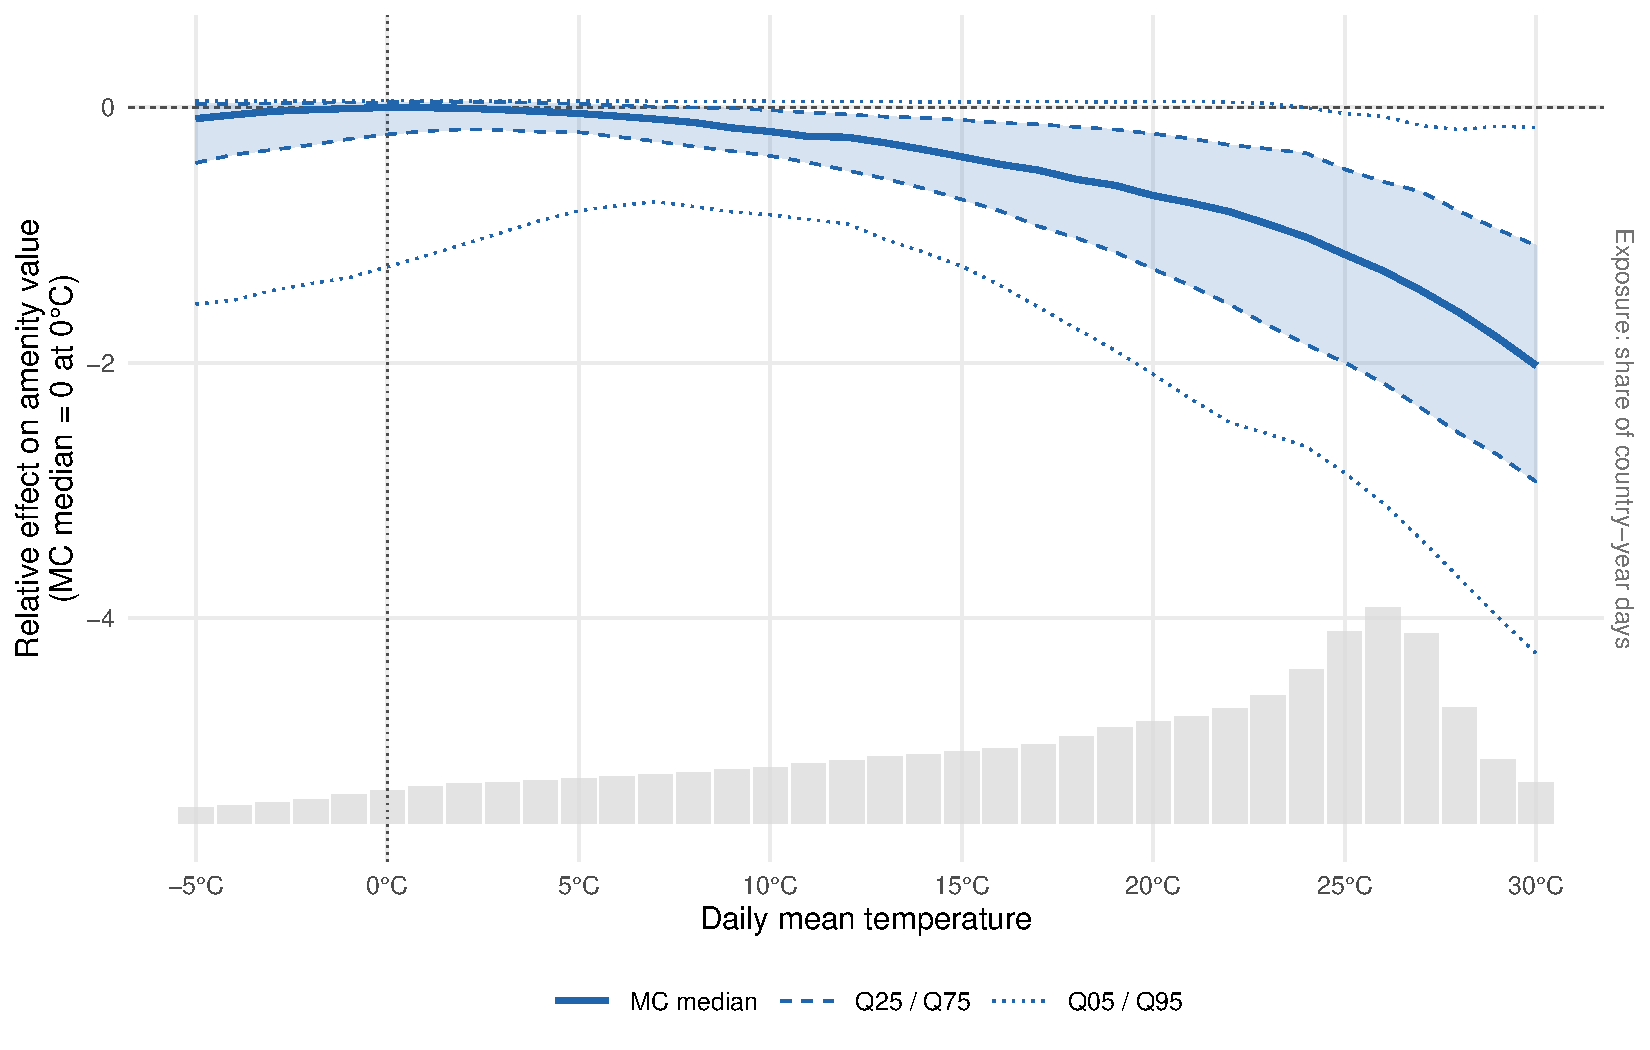
\includegraphics[width=\linewidth]{MC_amenity_daily_fan_paper.pdf}\\[-2pt]
  {\small (a) Daily temperature distribution}
\end{minipage}\hfill
\begin{minipage}[t]{0.49\textwidth}
  \centering
  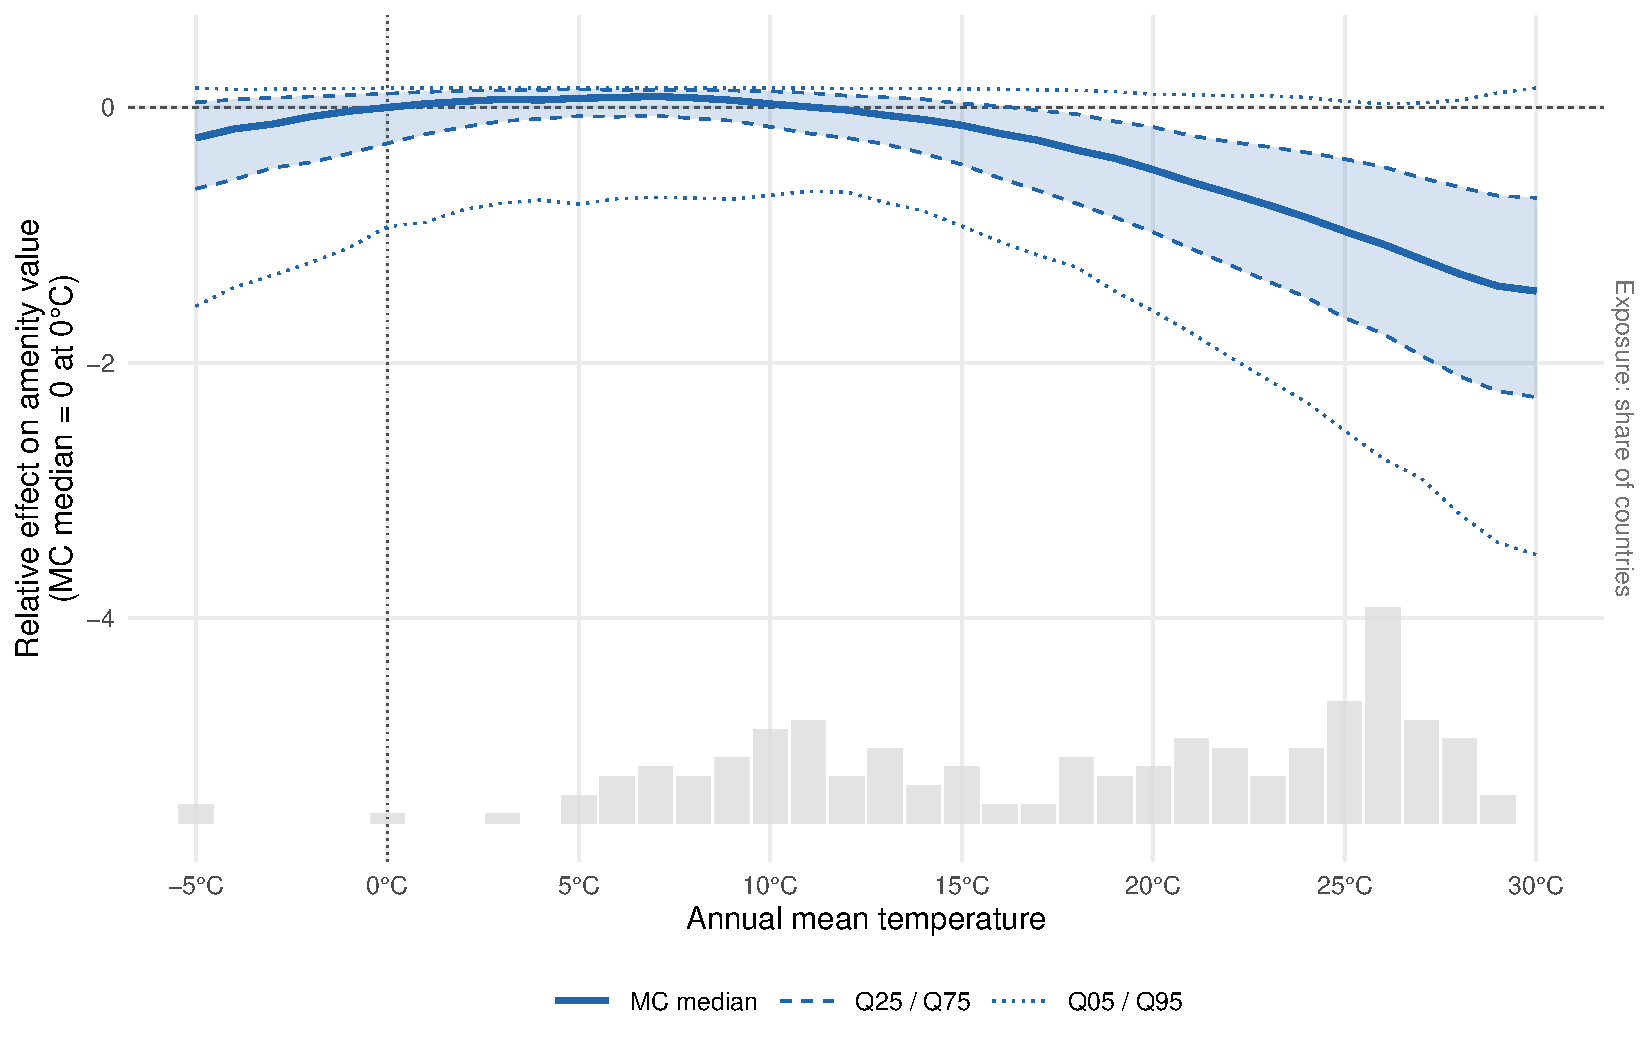
\includegraphics[width=\linewidth]{MC_amenity_annual_fan_paper.pdf}\\[-2pt]
  {\small (b) Annual mean temperature}
\end{minipage}
\caption{Amenity dose-response under the two exposure metrics. Monte Carlo
  ($\EMPnMC$ draws; specification sampled by Akaike weight, which is not
  degenerate here, then coefficients from $\mathcal N(\hat\beta,\hat V)$), each
  draw normalised to zero at $0^\circ$C; median, Q25--Q75 and Q05--Q95. Bars:
  the arm's own exposure. Axes cut at the common support.}
\label{fig:drf_amenity}
\end{figure}
%% ================================================================
\section{General-Equilibrium Details}
\label{supp:ge}
%% ================================================================

This section reports the GE results that
Section~\ref{sec:ge} summarises: the path between 2015 and \GEhorizonLabel, the
distribution across income groups, the full country and latitude tables, the
sensitivity to the amenity channel, the Monte Carlo band on the contrast, and
the decompositions behind Sections~\ref{sec:ge_gap} and~\ref{sec:ge_north}.
Unless stated otherwise, every run uses the amenity lower bound $f_a=0$. 

\subsection{Path and dispersion}
\label{supp:ge_path}

Table~\ref{tab:ge_aggregate} reports the three margins at 2030, 2050 and
\GEhorizonLabel. The annual total reaches $\GEaggAnnualThirty$ by 2030 and
$\GEworldAnnual$ by \GEhorizonLabel; the daily extra is negative at each of the three
horizons and grows in absolute value along the path, so that the daily
distribution adds losses rather than redistributing them. The share of the
world population living in cells with cumulative losses by \GEhorizonLabel\  is
$\GEpopLossDaily\%$ under the daily total, $\GEpopLossAnnual\%$ under the
annual total and $\GEpopLossExtra\%$ under the daily extra. The daily
distribution therefore adds losses for a majority of the world population but
not for all of it; in the remaining cells the intra-annual distribution
shifts in a way that partially offsets annual-mean damages. Its decisive
effect is at the sign margin: the share of the population in cells that gain
falls from $\GEpopGainAnnual\%$ to $\GEpopGainDaily\%$.


% GENERATED by 02_GE/emit_values.py -- DO NOT EDIT BY HAND
% amenity = none
\begin{table}[!ht]
\centering
\small
\caption{Aggregate welfare effects, population-weighted cumulative $\Delta\log U$, amenity lower bound $f_a = 0$. Daily extra is the difference of the two totals, computed before rounding, so the last digit of the three columns need not add up.}
\label{tab:ge_aggregate}
\begin{tabular}{lrrr}
\toprule
Horizon & Daily total & Annual total & Daily extra \\
        & (daily arm vs.~baseline) & (annual arm vs.~baseline) & (daily vs.~annual) \\
\midrule
2030 & $-0.003$ & $-0.001$ & $-0.002$ \\
2050 & $-0.010$ & $-0.004$ & $-0.005$ \\
2100 & $-0.017$ & $-0.008$ & $-0.010$ \\
\bottomrule
\end{tabular}
\end{table}


\subsection{Cold economies and latitude}
\label{supp:ge_north}
Table~\ref{tab:ge_latitude} reports the Northern aggregate at each threshold of the latitude grid. The contrast grows with latitude rather than sorting economies into categories: the colder the economy, the larger the annual-mean gain and the deeper the daily extra that removes it. 
% GENERATED by 02_GE/emit_values.py -- DO NOT EDIT BY HAND
% amenity = none
\begin{table}[!ht]
\centering
\small
\caption{Pop-weighted cumulative $\Delta\log U$ by 2100 across latitude bands, amenity lower bound $f_a = 0$.}
\label{tab:ge_latitude}
\begin{tabular}{lrrrr}
\toprule
Threshold & Pop. (M) & Annual total & Daily extra & Daily total \\
\midrule
$\geq 40^\circ$N & 1,112 & $+0.008$ & $-0.015$ & $-0.007$ \\
$\geq 45^\circ$N & 662 & $+0.011$ & $-0.018$ & $-0.006$ \\
$\geq 50^\circ$N & 375 & $+0.013$ & $-0.019$ & $-0.006$ \\
$\geq 55^\circ$N & 109 & $+0.023$ & $-0.027$ & $-0.003$ \\
$\geq 60^\circ$N & 18 & $+0.030$ & $-0.032$ & $-0.002$ \\
$\geq 66.5^\circ$N & 2 & $+0.033$ & $-0.033$ & $0.000$ \\
\bottomrule
\end{tabular}
\end{table}


\subsection{The amenity channel}
\label{supp:ge_amenity}

Tables~\ref{tab:ge_sensitivity} and~\ref{tab:ge_north_sens} re-run both
scenarios at the interior estimate $\hat f_a^{\,q50}$, the within-pair median
across specifications of the amenity dose-response that
Supplement~\ref{supp:amenity} shows to be unidentified. The world daily total
moves from $\GEworldDaily$ at the lower bound to $\GEworldDailyQfifty$, and
the annual total from $\GEworldAnnual$ to $\GEworldAnnualQfifty$, because the
interior estimate adds a congestion-adjusted amenity penalty across the
heterogeneous tropical population. For the Northern contrast the sign holds and
the magnitude does not: the daily extra above $45^\circ$N is
$\GEnorthExtraLB$ at the lower bound and $\GEnorthExtraQfifty$ at the
interior estimate, negative for every Northern economy under both and
\GEsensExtraRatio{} times deeper at the estimate; the Northern daily total runs
from $\GEnorthNetLB$ to $\GEnorthNetQfifty$ on the same comparison. At the interior estimate the annual arm itself projects $\GEnorthAnnualQfifty$ for the
aggregate: the annual amenity response carries no non-linearity the data support — the
test of its degree-two and higher terms has $p$ between \EMPamenAnnualPnonlinLo{} and
\EMPamenAnnualPnonlinHi{} across the grid, and the joint test of all its climate terms $p$
between \EMPamenAnnualPjointLo{} and \EMPamenAnnualPjointHi{} — so the position of its optimum, which decides
whether cold economies gain, is not identified, and the contrast does not rest on the
annual arm projecting a gain. Because
$\hat f_a$ lies \EMPamenScaleExcess{} times beyond the admissible bound and
below the threshold that Supplement~\ref{supp:amenity_identification} shows the
design could detect, this arm is a stress test past the restriction the paper
imposes on itself, not a point inside it.

% GENERATED by 02_GE/emit_values.py -- DO NOT EDIT BY HAND
% amenity = baseline+none
\begin{table}[!ht]
\centering
\small
\caption{Sensitivity of global pop-weighted cumulative $\Delta\log U$ by 2100 to the amenity specification}
\label{tab:ge_sensitivity}
\begin{tabular}{lrrr}
\toprule
Specification & Daily total & Annual total & Daily extra \\
\midrule
Interior estimate $\hat f_a^{\,q50}$ & $-0.218$ & $-0.153$ & $-0.065$ \\
Lower bound $f_a = 0$ & $-0.017$ & $-0.008$ & $-0.010$ \\
\bottomrule
\end{tabular}
\end{table}

% GENERATED by 02_GE/emit_values.py -- DO NOT EDIT BY HAND
% amenity = baseline+none
\begin{table}[!ht]
\centering
\small
\caption{Cumulative $\Delta\log U$ by 2100 for cold-climate economies under the two amenity specifications (interior $\hat f_a^{\,q50}$ vs.\ lower bound $f_a = 0$), in the order of Table~\ref{tab:ge}.}
\label{tab:ge_north_sens}
\begin{tabular}{lrrrr}
\toprule
        & \multicolumn{2}{c}{Annual total} & \multicolumn{2}{c}{Daily extra} \\
\cmidrule(lr){2-3}\cmidrule(lr){4-5}
Country & $\hat f_a^{\,q50}$ & $f_a = 0$ & $\hat f_a^{\,q50}$ & $f_a = 0$ \\
\midrule
Russia     & $-0.007$ & $+0.025$ & $-0.081$ & $-0.028$ \\
Finland    & $+0.012$ & $+0.027$ & $-0.071$ & $-0.028$ \\
Norway     & $-0.035$ & $+0.013$ & $-0.050$ & $-0.018$ \\
Sweden     & $-0.041$ & $+0.012$ & $-0.042$ & $-0.017$ \\
Canada     & $-0.080$ & $+0.011$ & $-0.073$ & $-0.021$ \\
Germany    & $-0.065$ & $+0.004$ & $-0.041$ & $-0.011$ \\
France     & $-0.108$ & $-0.008$ & $-0.040$ & $-0.004$ \\
\addlinespace
\textbf{North $\geq 45^\circ$N} & $\mathbf{-0.048}$ & $\mathbf{+0.011}$ & $\mathbf{-0.059}$ & $\mathbf{-0.018}$ \\
\bottomrule
\end{tabular}
\end{table}


\subsection{Band on ranked draws}
\label{supp:ge_band_ranked}
Table~\ref{tab:ge_band_ranked} solves the model at draws of the daily
dose-response. Three hundred coefficient vectors are drawn from the sandwich
covariance of the daily arm's estimate. The draws solved are a stratified sample at evenly spaced
percentiles of the projected Northern change in partial equilibrium, computed
for each draw by the function behind Figure~\ref{fig:contrast};
$\GEarmBnDraws$ of them are solved in general equilibrium. The
partial-equilibrium ordering carries over imperfectly (the Spearman
correlation between the partial-equilibrium ordering of the draws and the
ordering of their Northern daily totals in general equilibrium is
\GEarmBrankCorr) so the percentiles and shares reported are those of the
general-equilibrium outcomes.
The body reports the share of population in gaining cells for the central
run, $\GEpopGainDaily\%$. Across the draws the share has a median of
\GEpopGainDailyMed\% and reaches \GEpopGainDailyHi\% in the upper tail, above
the annual-mean central value.
%% GENERATED by 02_GE/emit_values.py -- DO NOT EDIT BY HAND.
%% amenity = none
\begin{table}[!ht]\centering\footnotesize
\setlength{\tabcolsep}{3pt}
\caption{Distribution of the general-equilibrium daily total by 2100 across Monte Carlo draws of the daily dose-response, cumulative population-weighted $\Delta\log U$.}
\label{tab:ge_band_ranked}
\begin{tabular}{lcccccccc}
\toprule
& \multicolumn{6}{c}{Daily total} & \multicolumn{2}{c}{Population in gaining cells (\%)} \\
\cmidrule(lr){2-7}\cmidrule(lr){8-9}
Unit & median & q05 & q95 & min & max & neg.\ draws & median & q95 \\
\midrule
World & $-0.018$ & $-0.029$ & $-0.005$ & $-0.034$ & $-0.0004$ & 60/60 & 0.3 & 20.0 \\
North $\geq 45^\circ$N & $-0.006$ & $-0.011$ & $-0.003$ & $-0.013$ & $-0.0002$ & 60/60 & 0.6 & 27.6 \\
North $\geq 55^\circ$N & $-0.004$ & $-0.008$ & $+0.0002$ & $-0.009$ & $+0.003$ & 56/60 & 2.7 & 60.8 \\
North $\geq 66.5^\circ$N & $0.000$ & $-0.005$ & $+0.004$ & $-0.006$ & $+0.007$ & 29/60 & 38.8 & 99.2 \\
Russia & $-0.003$ & $-0.008$ & $+0.0004$ & $-0.009$ & $+0.003$ & 55/60 & 0.8 & 65.1 \\
Finland & $-0.001$ & $-0.006$ & $+0.004$ & $-0.007$ & $+0.006$ & 38/60 & 13.4 & 100.0 \\
Canada & $-0.010$ & $-0.016$ & $-0.004$ & $-0.021$ & $-0.001$ & 60/60 & 0.2 & 1.7 \\
Germany & $-0.007$ & $-0.011$ & $-0.003$ & $-0.012$ & $-0.001$ & 60/60 & 0.0 & 0.0 \\
France & $-0.012$ & $-0.017$ & $-0.008$ & $-0.021$ & $-0.007$ & 60/60 & 0.0 & 0.0 \\
Norway & $-0.005$ & $-0.009$ & $-0.001$ & $-0.011$ & $+0.002$ & 59/60 & 5.1 & 20.0 \\
Sweden & $-0.005$ & $-0.009$ & $-0.0002$ & $-0.010$ & $+0.002$ & 57/60 & 0.6 & 31.5 \\
\bottomrule
\multicolumn{9}{p{\dimexpr\linewidth-2\tabcolsep\relax}}{\footnotesize
\textit{Note.} Distribution of the daily total across $\GEarmBnDraws$ Monte Carlo draws of the daily dose-response
(specification \EMPfigDrfSpecDaily), each solved in general
equilibrium with amenities at the lower bound and the no-climate
baseline common to all runs. Draws are a stratified sample of the
Monte Carlo distribution, taken at evenly spaced percentiles of the
projected Northern change in partial equilibrium. Percentiles and
shares are those of the general-equilibrium outputs.}
\end{tabular}
\end{table}


\subsection{Warming switched off by region}
\label{supp:exposure_masks}
Section~\ref{sec:ge_north} compares the headline runs with runs in which
warming is switched off in part of the world. Under the first mask, the
$\GEmaskNorthCells$ cells at or above $45^\circ$N keep their projected exposure
and the other $\GEmaskNonNorthCells$ cells keep their 2015 exposure in every
period; the second mask does the reverse. The model computes damage from the
change in exposure between periods, so a cell held at its 2015 exposure
receives no damage, as in the scenario without warming. Nothing else is
switched off: goods trade, migration, wages and congestion operate in every
cell, and each run is a full general-equilibrium solution under a partial
warming. Each mask is solved under the daily and the annual-mean function, at
the central draw of the dose-response and at the amenity lower bound $f_a=0$;
the run without warming is the headline one. These runs carry no Monte Carlo
band. The model is not linear, so the full-warming value need not equal the
sum of the two masked values; Section~\ref{sec:ge_north} reports the
difference, the interaction, with the shares.
\subsection{The two decompositions}
\label{supp:ge_decomp}
The two tables below carry quantities that the body reports and that no other
table does. The first is a difference between runs already described above.
The second reports the income component by latitude band and, above
$45^\circ$N, its share with warming confined to the North, from the masked runs
of Supplement~\ref{supp:exposure_masks}.

\begin{table}[H]\centering\small
\caption{Evaluation and function terms of the Northern daily extra
(Section~\ref{sec:ge_gap}). The third scenario applies the daily response to
annual-mean exposure, so the evaluation term is the part of the extra that the
change of exposure alone produces and the function term the remainder.}
\label{tab:ge_decomp_gap}
\begin{tabular}{lc}
\toprule
 & Cumulative $\Delta\log U$ \\
\midrule
Northern daily extra            & $\GEnorthDailyExtra$ \\
\quad evaluation term           & $\GEnorthChanEval$ \\
\quad function term             & $\GEnorthChanShape$ \\
\midrule
Ratio, function to evaluation   & $\GEnorthChanRatio$ \\
\bottomrule
\multicolumn{2}{p{\dimexpr0.8\linewidth\relax}}{\footnotesize
\textit{Note.} The two terms are \GEnorthChanSameSign{} one another. In
partial equilibrium the same split attributes $\EMPgapShareOfContrast\%$ of the
Northern contrast to the shape of the response, of which
$\EMPgapShareBelowZero\%$ lies below $0^\circ$C and $\EMPgapShareAboveTwenty\%$
above $20^\circ$C.}
\end{tabular}
\end{table}

\begin{table}[H]\centering\small
\caption{The income component of the daily extra by latitude band
(Section~\ref{sec:ge_north}), at the central draw of the dose-response. Each
entry is the income component for the cells of the band; the last column is
its value with warming confined to cells at or above $45^\circ$N, as a share of
its value when the whole world warms.}
\label{tab:ge_decomp_lat}
\begin{tabular}{lcc}
\toprule
Latitude band & Income component & Northern warming only (\%) \\
\midrule
Below $30^\circ$N          & $\GEchanIncomeTrop$ & --- \\
$30$--$45^\circ$N          & $\GEchanIncomeMid$  & --- \\
$45$--$60^\circ$N          & $\GEchanIncomeSub$  & $\GEmaskNorthWarmingIncomeSubShare$ \\
Above $60^\circ$N          & $\GEchanIncomeArc$  & $\GEmaskNorthWarmingIncomeArcShare$ \\
\bottomrule
\multicolumn{3}{p{\dimexpr0.8\linewidth\relax}}{\footnotesize
\textit{Note.} The share is not reported below $45^\circ$N, where the cells do
not warm under that mask.}
\end{tabular}
\end{table}

\section{The Cruz--Rossi-Hansberg Pipeline}
\label{supp:crh}
%% ================================================================

The bilateral estimator identifies the productivity dose-response from a cross-section of
trade flows between countries, and its vulnerability is the confounding specific to that
cross-section. This section re-runs the contrast in a design that shares neither its data,
nor its unit, nor its fundamental: the estimation of \citet{cruz2024economic} on
model-inverted cell fundamentals, under their fixed effects --- sub-region$\times$period for
productivity, blocks of $2\times2$ cells and sub-country$\times$period for amenities ---
with a single lever moved, the exposure metric. The design has no cell fixed effect:
identification is across cells within a sub-region and period, with
\EMPcrhWithinCellProd\% of the identifying variance of the productivity regressors and
\EMPcrhWithinCellAmen\% of the amenity regressors lying within cells across periods
(\EMPcrhWithinCellTmeanProd\% and \EMPcrhWithinCellTmeanAmen\% for the mean temperature).

I invert the \citet{cruz2024economic} model to recover productivities
$\bar a_t(r)$ and amenities $\bar b_t(r)$ on their $1^\circ$ grid
($\EMPcrhGridCells$ cells, four decadal cross-sections 1990--2005,
$\EMPcrhCellPeriods$ cell-periods), following \citet{desmet2018geography};
I use my own inversion rather than the deposited fundamentals so that
inversion, estimation and projection are internal to one reproduction.
Re-estimating the authors' own specification (a ten-year mean of the
coldest-month temperature) on my inversion reproduces their bliss points
($\EMPcrhOptProd^\circ$C against $1.6^\circ$C for productivity,
$\EMPcrhOptAmen^\circ$C against $8.6^\circ$C for amenities).
The daily arm follows \citet{schlenker2009nonlinear}: the fundamental
is regressed on the shares of days in each temperature bin,
$\sum_k\hat\delta_k s_k(r)$, under the authors' fixed effects and geographic
controls, and the $\hat\delta_k$ are re-estimated, not plugged in from the
annual function. The two metrics agree in their first moment: the cell mean
of the ERA5 daily distribution reproduces the authors' own decadal average
temperature with correlation $\EMPcrhMetricCor$, slope $\EMPcrhMetricSlope$
and bias $\EMPcrhMetricBias^\circ$. The authors cluster spatially (Conley, 550~km). Every interval reported here
clusters at the country level. The projection is linear in the estimated coefficients, so
the interval on the difference between arms carries their covariance
(correlation \EMPcrhCorArmsLo\ to \EMPcrhCorArmsHi) rather than treating them
as independent.

Figure~\ref{fig:crh_response} plots the re-estimated damage functions.

\begin{figure}[!ht]
\centering
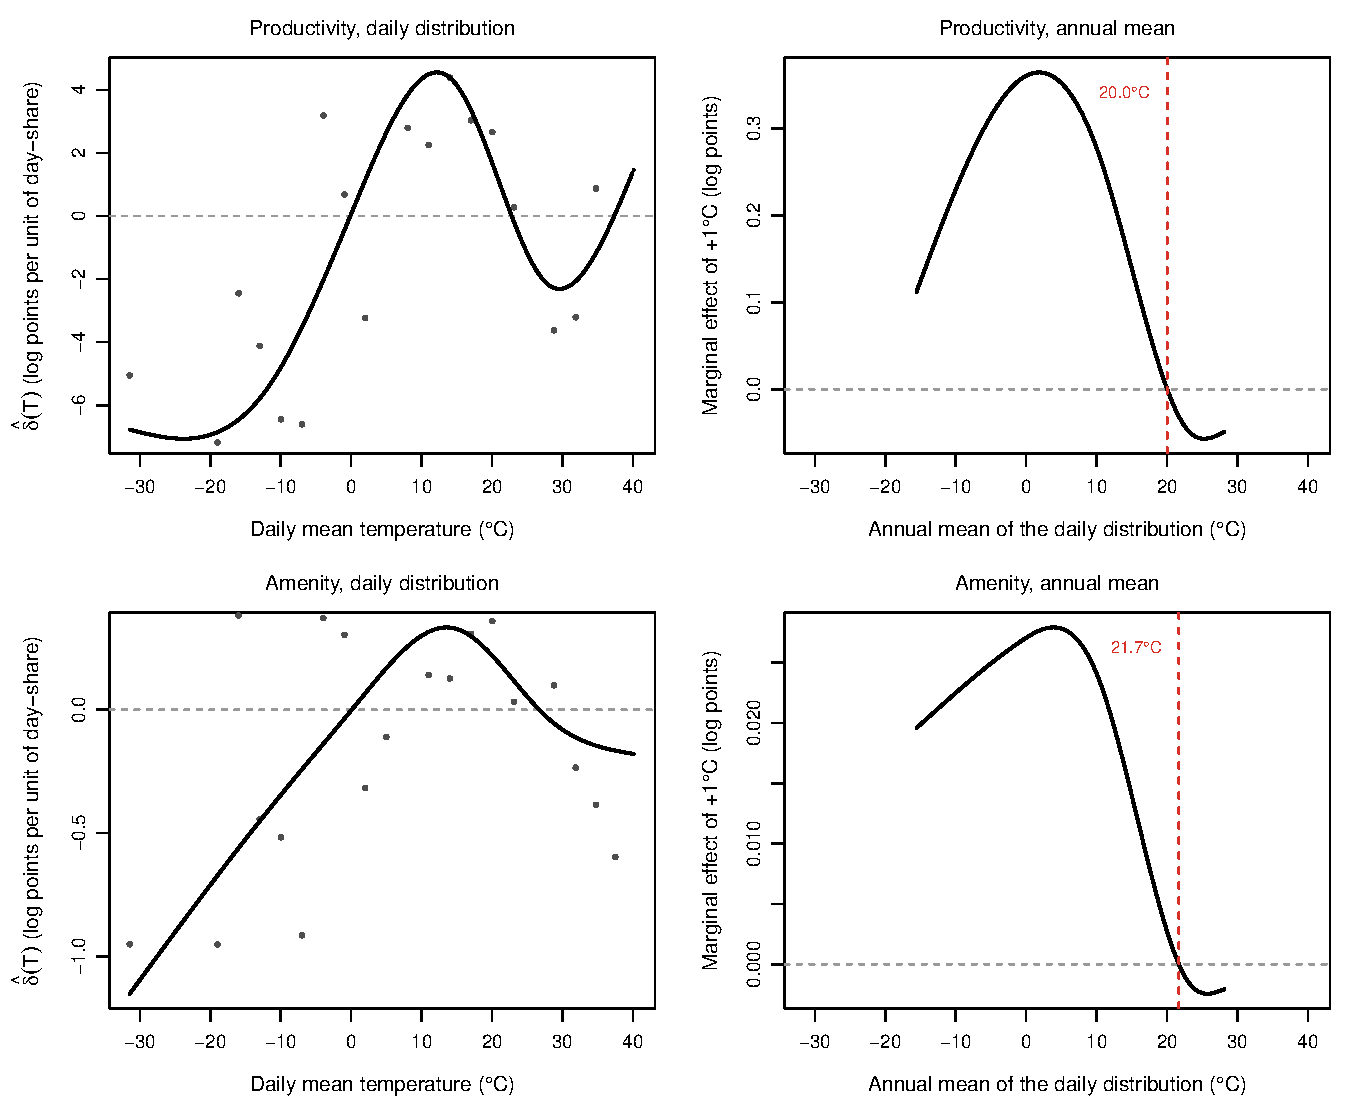
\includegraphics[width=\textwidth]{fig_crh_responses.pdf}
\caption{Productivity (top) and amenities (bottom), under the
  daily-distribution metric (left) and the annual-mean metric (right).
  Left: the effect on the change in the log fundamental of shifting one unit
  of day-share into temperature $T$, relative to the reference bin at
  \EMPcrhDailyRefBin{}$^\circ$C;
  points are bin coefficients, the line a weighted natural-spline fit. Right: the effect on the same object of a
  one-degree rise in the annual mean. Columns
  differ and their vertical scales are not comparable.}
\label{fig:crh_response}
\end{figure}


In the day-response
$\hat\delta(T)$, an additional day is most valuable near
$\EMPcrhPeakProd^\circ$C for productivity and $\EMPcrhPeakAmen^\circ$C for
amenities, and its value declines above $20$--$25^\circ$C. As a cold
cell warms, its distribution grows an upper tail into that declining region,
which an evaluation at the mean cannot register. Across baseline temperatures the daily projection lies below the annual-mean one, and in the temperate band the two disagree in sign at the cell level. The upper tail is data-poor in the estimation sample,
the mirror image of the cold-branch caveat of Supplement~\ref{supp:productivity};
I hold $\hat\delta(T)$ flat beyond $\EMPcrhSupportHi^\circ$C, the hottest bin
with at least $1\%$ of cell-periods, and $\EMPcrhNorthDayMassAboveSupport\%$ of the cold
economies' projected day-mass lies beyond it: clamping moves the Northern
aggregate by $\EMPcrhClampMove$. Holding $\hat\delta(T)$ flat beyond $30^\circ$C instead moves the Northern
difference by $\EMPcrhClampThirtyMove$, and
\EMPcrhNorthDayMassAboveThirty\% of the day-mass of cells above $45^\circ$N
lies above $30^\circ$C by \GEhorizonLabel{}: the upturn of the fitted
response between $30$ and $40^\circ$C, which rests on a few bins with little
mass, plays no part in the Northern result.

The shape of the annual-mean response in Figure~\ref{fig:crh_response}
differs from the authors' published one, and the difference is a property of the fitting, not of the data. The
authors fit to their twenty bin slopes a logistic function whose slope
parameter is fixed, so that the estimated response is a smooth step by
construction: flat at the cold end, flat at the hot end, and a single
transition whose centre is the bliss point. The annual arm here smooths the
same kind of bin slopes with a natural spline, which imposes no shape, and
what it shows is that the marginal effect of warming is largest at annual
means between $0$ and $10^\circ$C and weakens towards the coldest cells,
below $-10^\circ$C, where few cells lie and the slope is poorly estimated
under either specification. The two responses also sit on different
supports: in the authors' winter-month metric the Siberian cells lie
between $-40$ and $-20^\circ$C, on the flat upper plateau of the logistic,
whereas in the annual mean the same cells lie between $-15$ and
$0^\circ$C, where the spline turns down. What the two fits agree on is
what the projection uses: the marginal effect is positive throughout the
North and negative in the tropics, and its zero crossing (at
\EMPcrhMeanOpt{}$^\circ$C in annual-mean terms, \EMPcrhOptProd{}$^\circ$C
in the authors' winter-month terms) separates the same cells. I keep the spline rather than adopt the authors' logistic for the annual
arm. Imposing their functional form would reproduce the appearance of
their figure, but it would do so by ruling out what the bin slopes show:
that the marginal effect of warming weakens in the coldest cells. The
spline reports that feature and the logistic cannot; where the two agree,
on the sign and the crossing, the choice is immaterial, and where they
differ, the spline follows the data.

Table~\ref{tab:crh_north} reports the projected change in the log fundamental
between 2015 and \GEhorizonLabel\  under SSP2-4.5 for the five largest cold economies and
the aggregate above $45^\circ$N. The projection runs to \GEhorizonLabel\  rather
than the authors' 2200, uses SSP2-4.5 rather than RCP~8.5, and is a
partial-equilibrium projection of the fundamental without their endogenous
innovation.

\begin{table}[!ht]
\centering\small
\caption{Projected change in the log fundamental, \GEhorizonSpan (SSP2-4.5), in
  the Cruz--Rossi-Hansberg pipeline: annual-mean versus daily-distribution
  metric and their difference. Partial-equilibrium projection, four-period
  sample, 95\% intervals clustered by country.}
\label{tab:crh_north}
%% GENERATED by 01d_crh_triangulation.R -- DO NOT EDIT BY HAND.
\begin{tabular}{lccc}
\toprule
Region & Annual mean & Daily & Difference \\
\midrule
\multicolumn{4}{l}{\emph{Productivity}} \\
Russia & $+0.778$ & $+0.247$ & $+0.531$ \\
 & {\footnotesize $[+0.310,\,+1.258]$} & {\footnotesize $[-0.140,\,+0.635]$} & {\footnotesize $[+0.311,\,+0.754]$} \\
\addlinespace[2pt]
Canada & $+0.790$ & $+0.171$ & $+0.618$ \\
 & {\footnotesize $[+0.287,\,+1.307]$} & {\footnotesize $[-0.248,\,+0.591]$} & {\footnotesize $[+0.359,\,+0.883]$} \\
\addlinespace[2pt]
Finland & $+0.670$ & $+0.379$ & $+0.291$ \\
 & {\footnotesize $[+0.274,\,+1.075]$} & {\footnotesize $[+0.027,\,+0.728]$} & {\footnotesize $[+0.071,\,+0.515]$} \\
\addlinespace[2pt]
Germany & $+0.441$ & $+0.095$ & $+0.347$ \\
 & {\footnotesize $[+0.104,\,+0.789]$} & {\footnotesize $[-0.212,\,+0.394]$} & {\footnotesize $[+0.103,\,+0.592]$} \\
\addlinespace[2pt]
France & $+0.297$ & $-0.187$ & $+0.484$ \\
 & {\footnotesize $[+0.015,\,+0.584]$} & {\footnotesize $[-0.453,\,+0.071]$} & {\footnotesize $[+0.264,\,+0.712]$} \\
\addlinespace[2pt]
North $\geq$45N & $+0.559$ & $+0.116$ & $+0.443$ \\
 & {\footnotesize $[+0.186,\,+0.943]$} & {\footnotesize $[-0.184,\,+0.414]$} & {\footnotesize $[+0.238,\,+0.651]$} \\
\addlinespace[2pt]
\addlinespace
\multicolumn{4}{l}{\emph{Amenity}} \\
Russia & $+0.063$ & $+0.033$ & $+0.031$ \\
 & {\footnotesize $[+0.000,\,+0.126]$} & {\footnotesize $[-0.006,\,+0.072]$} & {\footnotesize $[-0.012,\,+0.074]$} \\
\addlinespace[2pt]
Canada & $+0.066$ & $+0.028$ & $+0.038$ \\
 & {\footnotesize $[-0.001,\,+0.132]$} & {\footnotesize $[-0.011,\,+0.066]$} & {\footnotesize $[-0.007,\,+0.084]$} \\
\addlinespace[2pt]
Finland & $+0.054$ & $+0.036$ & $+0.018$ \\
 & {\footnotesize $[+0.001,\,+0.107]$} & {\footnotesize $[+0.006,\,+0.066]$} & {\footnotesize $[-0.016,\,+0.052]$} \\
\addlinespace[2pt]
Germany & $+0.039$ & $+0.015$ & $+0.024$ \\
 & {\footnotesize $[-0.003,\,+0.081]$} & {\footnotesize $[-0.008,\,+0.038]$} & {\footnotesize $[-0.004,\,+0.053]$} \\
\addlinespace[2pt]
France & $+0.028$ & $-0.004$ & $+0.032$ \\
 & {\footnotesize $[-0.006,\,+0.062]$} & {\footnotesize $[-0.028,\,+0.020]$} & {\footnotesize $[+0.005,\,+0.060]$} \\
\addlinespace[2pt]
North $\geq$45N & $+0.047$ & $+0.019$ & $+0.028$ \\
 & {\footnotesize $[-0.001,\,+0.096]$} & {\footnotesize $[-0.006,\,+0.044]$} & {\footnotesize $[-0.003,\,+0.060]$} \\
\addlinespace[2pt]
\addlinespace
\bottomrule
\end{tabular}

\end{table}



\end{document}
